\graphicspath{{chapt_dutch/}{intro/}{sm_beyond/}{chapt3/}{chapt4/}{chapt5/}{chapt6/}{chapt7/}{chapt8/}}

% Header
\renewcommand\evenpagerightmark{{\scshape\small Chapter 2}}
\renewcommand\oddpageleftmark{{\scshape\small The Standard Model and Beyond}}
%\newcommand\slashzero{\stackinset{c}{}{c}{}{/}{0}}
\renewcommand{\bibname}{References}

\hyphenation{}

\chapter[The Standard Model and beyond]%
{The Standard Model and Beyond}\label{chapt:2}
This chapter describes the Standard Model (SM) of particle physics, the physics of top quark and the SM Higgs boson. The discussion follows the introduction to the SM extension, SUSY, MSSM, and model-dependent heavy Higgs searches. The last part is devoted to the search of neutral heavy Higgs decays into a pair of top quarks ($H \rightarrow t\bar{t}$) with QCD $t\bar{t}$ interference, observables for signal and background discrimination and sensitivity at higher luminosities.    
\section{The Standard Model}\label{sec:sm}
The SM theory describes matter in terms of elementary particles, fermions, all having a half-integer spin and the three fundamental forces with mediators and gauge bosons (integer spin). Fermions are further divided into two classes based on their properties – quarks and leptons. The three fundamental forces are electromagnetic (EM); strong; and weak; and they are mediated by photon, gluon, and gauge bosons (W$^{\pm}$, Z) respectively. The Higgs mechanism is an important and fundamental feature of the SM to describe symmetry breaking that is responsible for giving masses to all fundamental particles. 
The discovery of the SM Higgs boson by the CMS and ATLAS experiments~\cite{cms_sm_higgs,atlas_sm_higgs} in 2012 at the LHC at CERN solved the mystery. The most familiar force, `` gravity'', is not included in the SM because the current energy scale of the accelerators can't cope with strength of gravity at a particle level, which is extremely weak as compared to the strong force (10$^{38}$). The SM of particle physics is a renormalizable quantum field theory based on a local unitary product group SU(3)$\times$SU(2)$\times$U(1), where the subgroup SU(3) represents the strong interaction and SU(2)$\times$U(1) is the unification of the electromagnetic and weak interaction (electroweak). Table~\ref{table:sm} provides a summary of the SM particles along with their properties; the three fundamental forces are described in the following section. 
  \begin{table}[h!]%\footnotesize
\centering
     %\begin{tabular}{|p{1.4cm}|p{1.0cm}|p{1.0cm}|}
    \tabulinesep=1.0mm
     \begin{tabu}{|l|c|c|c|c|}
    \hline
    \multicolumn{5}{ |c| }{Leptons} \\
    \hline\hline
    Particle & Spin & Charge & Interaction & Mass (GeV)\\
\hline 
Electron (e)& $\frac{1}{2}$ & $-$1 & e, w & 0.511 $\times$ 10$^{-3}$\\ 
\hline
Electron Neutrino ($\nu_{e}$) & $\frac{1}{2}$ & 0 & w & < 2.20 $\times$ 10$^{-9}$\\ 
\hline
Muon ($\mu$)   & $\frac{1}{2}$ & $-$1 & e, w & 0.105\\
\hline
Muon Neutrino ($\nu_{\mu}$)  & $\frac{1}{2}$ & 0 & w & < 0.17 $\times$ 10$^{-6}$\\
\hline
Tau ($\tau$)     & $\frac{1}{2}$ & $-$1 & e, w & 1.776 \\
\hline
Tau Neutrino ($\mu_{\tau}$)    & $\frac{1}{2}$ & 0 & w  & < 15.5 $\times$ 10$^{-6}$\\
\hline\hline
		\multicolumn{5}{ |c| }{Quarks} \\
		\hline\hline
        Particle & Spin & Charge & Interaction & Mass (GeV)\\
\hline
Up Quark (u)      & $\frac{1}{2}$ & $+\frac{2}{3}$ & c, e, w & 2.2 $\times$ 10$^{-3}$\\ 
\hline
Down Quark (d)    & $\frac{1}{2}$ & $-\frac{1}{3}$ & c, e, w & 4.7 $\times$ 10$^{-3}$ \\ 
\hline
Charm Quark (c)   & $\frac{1}{2}$ & $+\frac{2}{3}$  & c, e, w & 1.27\\  
\hline
Strange Quark (s) & $\frac{1}{2}$ & $-\frac{1}{3}$  & c, e, w & 96.0 $\times$ 10$^{-3}$\\
\hline
Top Quark (t)     & $\frac{1}{2}$ & $+\frac{2}{3}$  & c, e, w & 173.2\\ 
\hline
Bottom Quark (b)  & $\frac{1}{2}$ & $-\frac{1}{3}$  & c, e, w & 4.18\\     
\hline\hline
 		\multicolumn{5}{ |c| }{Gauge Bosons} \\
 		\hline\hline
        Particle & Spin & Charge & Interaction & Mass (GeV)\\
\hline
Photon ($\gamma$)      & 1 & 0 & e & 0\\ 
\hline
W Boson (W)     & 1 & $\pm$1 & e, w & 80.3\\ 
\hline
Z Boson (Z)      & 1 & 0 & w & 91.1\\ 
\hline
Gluon (g)      & 1 & 0 & c & 0\\ 
\hline
        \hline
        \multicolumn{3}{ |c| }{Scalar Bosons} \\
        \hline\hline
        Particle & Spin & Charge & Interaction & Mass (GeV)\\
\hline
Higgs Boson (h)      & 0 & 0 & w & 125.5\\
        \hline
     \end{tabu}
     \caption{ Summary of the SM of particle physics. First column – particle name (symbol); second column – spin; third column – charge; fourth column – corresponding interaction, where c stands for colour, e for electromagnetic, and w for weak force. The last column shows masses of the particles. The values are taken from the Particle Data Group (PDG)~\cite{sm_pdg}.\label{table:sm}}
%\end{center}
\end{table}  
\begin{itemize}
\item{\textbf{Strong Nuclear Force}}: is the fundamental force experienced by quarks and gluons, where the colour quantum numbers (red, blue, green) of particles play an important role, such as a particle charge in electromagnetism. It is responsible for binding quarks inside the nucleus via exchange of gluons within a short range of 10$^{-15}$\,m. The force is independent of the charge of particles and is explained by the Quantum Chromodynamics (QCD) theory. QCD depends on the non-Abelian gauge group SU(3); hence, gluons are self-interacting. The strength of the strong coupling constant is $\sqrt{4\pi\alpha_{s}(Q^{2})} $ and the coupling constant is, in fact, not constant at all but depends on the separation distance between the particles, known as the ``running'' coupling constant. The strong coupling constant increases at a short distance (the size of proton) and decreases when the distance becomes large. This phenomenon is known as $\textbf{asymptotic freedom}$. QCD plays a key role in the high-energy physics regime that is present in the LHC where the colliding particles are hadrons (protons). The full Lagrangian of QCD is given in Eq.~\ref{eq:qcd_lagrange}:
\begin{equation}
\begin{split}
\mathcal{L}_{QCD} & = -\frac{1}{4}(\partial^{\mu}G^{\nu}_{a} - \partial^{\nu}G^{\mu}_{a})(\partial_{\mu}G_{\nu}^{a} - \partial_{\nu}G_{\mu}^{a}) + \sum\limits_{f}q^{-\alpha}_{f}(i\gamma^{\mu}\partial_{\mu} - m_{f})q^{\alpha}_{f} \\
& + g_{s}G^{\mu}_{a} \sum\limits_{f} q^{-\alpha}_{f}\gamma_{\mu}\bigg(\frac{\lambda^{a}}{2}\bigg)_{\alpha\beta}q^{\beta}_{f}\\
& - \frac{g_{s}}{2}f^{abc}(\partial^{\mu}G^{\nu}_{a} - \partial^{\nu}G^{\mu}_{a})G_{\mu}^{b}G_{\nu}^{c} - \frac{g_{s}^{2}}{4}f^{abc}f_{ade}G^{\mu}_{b}G^{\nu}{c}G^{d}{\mu}G^{e}_{\nu}
\end{split}\label{eq:qcd_lagrange} 
\end{equation}    
The first line involves the correct kinetic terms for the different fields, which give rise to the corresponding propagators. The second line contains SU(3)$_{C}$ matrices and $\lambda^{a}$ provides the colour interaction between gluons and quarks. The last line gives the self-interactions in gluons generated by G$^{\mu\nu}_{a}$G$_{\mu\nu}^{a}$; g$_{s}$ is the strength of the coupling constant~\cite{strong_force}. 

\item{\textbf{Electromagnetic Interaction}}: is a fundamental long-range force that acts upon charge particles and is mediated by virtual photons. It is described by the Quantum Electrodynamics (QED) theory, based on Abelian gauge group U(1)$_{EM}$, where the coupling constant is $\alpha = \frac{e^{2}}{4\phi} \approx \frac{1}{137}$, much smaller than unity, where ``e'' shows the electric charge of particle. The coulomb force between the two static charged particles, $q_1$ and $q_2$, is given by Eq.~\ref{equ:qed}:
\begin{equation}\label{equ:qed}
F = k\frac{q_1 q_2}{r^2}
\end{equation}
Where $k$ is the proportionality constant and $r$ is the distance between the centre of the charged particles.
An example of QED is the Bhabha scattering of the $e^{+}e^{-} \rightarrow e^{+}e^{-}$, as shown in Fig.\ref{fig:electro_force}.
\begin{figure}[h!]
\centering
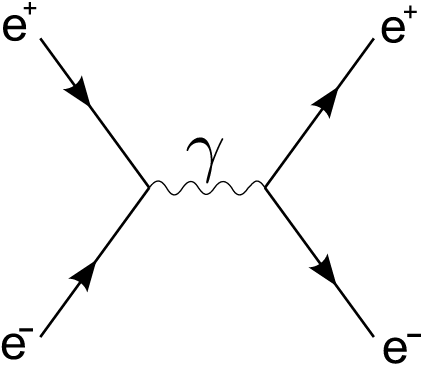
\includegraphics[width=0.35\textwidth]{fig/sm_beyond/electromagnetic.png}
%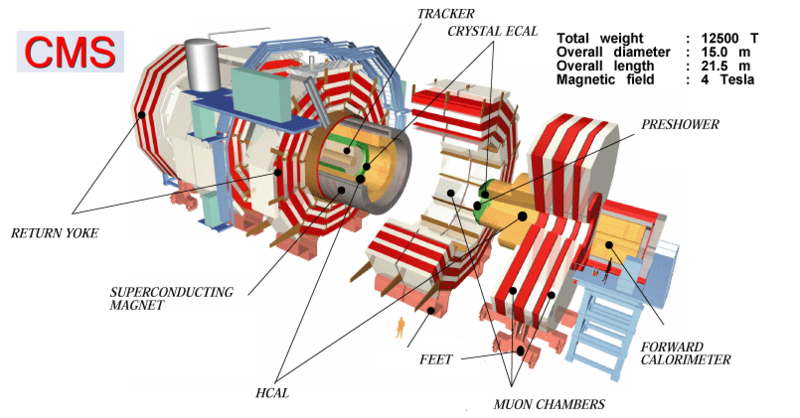
\includegraphics[scale=0.4, trim=20 50 60 30,clip]{fig/chapt3/CMS_exper.png}
\caption{\label{fig:electro_force} An overview of the Bhabha scattering in QED.}
\end{figure}
\item{\textbf{Weak Interaction}}:
All fundamental particles, except gluon (g) and photon ($\gamma$), experience weak interactions by exchanging or producing W$^{\pm}$ or Z bosons. It is a short-range (10$^{-17}$ to 10$^{-16}$\,m) interaction and responsible for many phenomena, such as radioactivity. Weak isospin, given in Eq.~\ref{eq:weak_isospin}, conserves in weak interaction and plays a similar role in weak interactions as colour and charge in strong and electromagnetic interactions respectively. In case of leptons, the theory is very clear, like the decay of muon mediated by W$^{-}$ boson ($\mu^{-} \rightarrow e^{-} + \nu_{\mu} + \bar{\nu_{e}}$) and electron-neutrino scattering via Z boson ($\nu_{\mu} + e^{-} \rightarrow \nu_{\mu} + e^{-}$). The lepton number is conserved in both processes. A similar model is applied to three generations of quarks, where a quark converts into the same generation; but in nature, cross-generation conversion is observed. The dilemma was solved by introducing the 3 $\times$ 3 $\textbf{CKM}$ (Cabibbo–Kobayashi–Maskawa) matrix~\ref{eq:ckm1}, with diagonal elements very near to unitary.
\begin{equation}\label{eq:ckm1}
\left({\begin{array}{ccc} \rm d' \\ \rm s' \\ \rm b' \end{array}}\right) = 
	  \left( \begin{array}{ccc}
      \rm  V_{ud} &\rm V_{us} &\rm V_{ub}\\
      \rm  V_{cd} &\rm V_{cs} &\rm V_{cb}\\
      \rm  V_{td} &\rm V_{ts} &\rm V_{tb}\end{array} \right)
\left({\begin{array}{ccc} \rm d \\ \rm s \\ \rm b \end{array}}\right)
\end{equation}  
Down-type quarks ($\rm d', \rm s', \rm b'$) are a superposition of down-type quarks following Eq.\ref{eq:ckm1} and couple to up-type quarks via charged current weak interaction. The matrix elements provide the rate at which one quark converts to another, e.g. $\rm V_{ud}$ gives the transition rate of $d \rightarrow u$. All the nine CKM matrix values are given in Eq.~\ref{eq:ckm2}.
\begin{equation}\label{eq:ckm2}    \small 
\rm V_{\rm CKM}	=  \left( \begin{array}{ccc}
      \rm  0.97434_{-0.00012}^{+0.00011} &\rm 0.22506\pm 0.0005&\rm 0.00357\pm 0.00015\\
      \rm  0.22492\pm 0.0005 &\rm 0.97351\pm 0.00013 &\rm 0.0411\pm 0.0013\\
      \rm  0.00875_{-0.00033}^{+0.00032} &\rm 0.0403\pm 0.0013 &\rm 0.99915\pm 0.00005\end{array} \right)
\end{equation}
The diagonal elements are $\approx$1, which shows that the transition in the same generation is dominant~\cite{ckm}.
\item{\textbf{The Electroweak Symmetry:}}
The electromagnetic and weak forces were combined by Glashow, Weinberg, and Salam through a unique gauge electroweak theory (GWS) based on the SU(2)$_{L}\times \text{U}(1)_{Y}$ group~\cite{gws}. The theory introduces three SU(2)$_{L}$ gauge bosons W$^{i}_{\mu}$, i = 1,2,3, with coupling strength g$_{w}$, and one U(1)$_{Y}$ gauge boson, B$_{\mu}$, with coupling constant g$'$/2. The GWS theory depends upon the chirality of particles, which means that it transforms left-handed particles as doublets with weak isospin (I) $\pm\frac{1}{2}$ and right-handed particles as singlet with I = 0. The hypercharge (Y) and the third component of weak isospin (I$^{3}$) are related to charge (Q in unit of e) as:
\begin{equation}\label{eq:weak_isospin}
Q = I^{3} + \frac{1}{2}Y
\end{equation}  
The wave functions of the charged fields W$^{\pm}_{\mu}$, neutral field Z$_{\mu}$, and photon A$_{\mu}$ are represented by:
\begin{equation}
\begin{split}
W^{\pm}_{\mu} = \frac{1}{\sqrt{2}}\left( W_{\mu}^{1} \mp W_{\mu}^{2}\right)\\
Z_{\mu} = \left( W_{\mu}^{3}\cos\theta_{w} - B_{\mu}\sin\theta_{w}\right)\\
A_{\mu} = \left( W_{\mu}^{3}\sin\theta_{w} + B_{\mu}\cos\theta_{w}\right)
\end{split}\label{eq:electroweak}
\end{equation}   
Where $\theta_{w}$ is the weak mixing angle given in terms of electromagnetic coupling constant (g$_{e}$) as:
\begin{equation}
g_{w}\sin\theta_{w} = g'\cos\theta_{w} = g_{e} 
\end{equation} 
In GWS theory, breaking of the underlying SU(2)$_{L}\times \text{U}(1)_{Y}$ symmetry predicts the existence of two charged gauge fields and two neutral gauge fields shown in Eq.~\ref{eq:electroweak}.  
\item{\label{item:higgs_mechanism}\textbf{The Higgs Mechanism:}} SM is based on gauge invariance that forbids introducing explicit mass terms in the Lagrangian of a chiral theory, as it breaks the symmetry. This results to massless SM particles – a contradiction to nature. A mechanism is needed for introducing the mass term in the SM without spoiling the gauge symmetry, known as the Higgs mechanism published by three groups independently and therefore also called the Brout-Englert-Higgs (BEH) mechanism~\cite{eng_brout,p_w_higgs}. The GWS uses the BEH mechanism that introduces a new doublet of complex scalar field, known as the Higgs field, preserves symmetry under the gauge transformations, and acquires a non-zero vacuum expectation value, spontaneous electroweak symmetry breaking. The Higgs field contains a total of four additional degrees of freedom, where three of them become massive, given by the relation~\ref{eq:electroweak}, after breaking the symmetry and one remains massless, the photon $\gamma$. The Higgs doublet introduced in the SU(2)$_{L}$ with hypercharge (Y = $\frac{1}{2}$) is in the form of:
\begin{equation}
\phi = \Big(\begin{array}{c}
\phi^{+}\\
\phi^{0} \end{array}\Big)
= \frac{1}{\sqrt{2}}
\Big(\begin{array}{c}
\phi^{1} + i\phi^{2}\\
\phi^{3} + i\phi^{4}
\end{array}\Big)
\end{equation}
The SM electroweak Lagrangian density is given in term of
\begin{equation}\label{eq:beh_lagrange}
\mathcal{L}_{BEH} = (D^{\mu}\phi)^{\dagger}(D_{\mu}\phi) - V(\phi), \quad \textrm{with}\quad 
        V(\phi) = \mu^{2}\phi^{\dagger}\phi + \lambda(\phi^{\dagger}\phi)^{2}
\end{equation}
Where the first term of the Lagrangian D$^{\mu}$ corresponds to the covariant derivative of the Higgs field under the SU(2) $\times$ U(1) group, and the second term is the scalar potential known as ``Mexican Hat'' potential, shown graphically in Fig.~\ref{fig:mexican_hat}. 
\begin{figure}[h]
\centering
\captionsetup{width=0.8\linewidth}
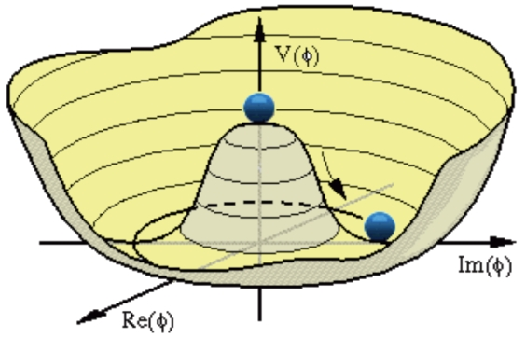
\includegraphics[width=0.4\textwidth]{fig/sm_beyond/mexican_hat.png}
%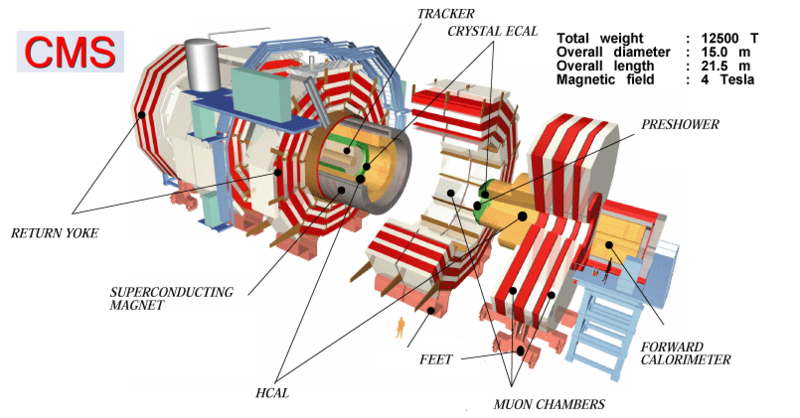
\includegraphics[scale=0.4, trim=20 50 60 30,clip]{fig/chapt3/CMS_exper.png}
\caption{\label{fig:mexican_hat}The scalar potential V($\phi$)with $\mu^{2}$ < 0 has a ``Mexican hat shape'', with the minimum in a rim around the origin. Moving from the origin down to the minimum, the symmetry breaks and the scalar field acquires a vacuum expectation value (vev) in the process}
\end{figure}
The Higgs potential has chosen to achieve the necessary spontaneous symmetry breaking in the simplest form while being renormalizable. The Higgs potential V($\phi$) depends on the values of $\lambda$ and $\mu^{2}$. For a stable vacuum, the parameter $\lambda$ has to be a positive value. If $\mu^{2}$ > 0, the scalar potential has a global minimum, $\langle 0\abs{\phi}0\rangle = 0$, where no spontaneous symmetry breaking occurs. While for $\mu^{2} < 0$, the symmetry breaks and the Higgs field acquires a non-zero vacuum expectation value with conditions $\langle 0\abs{\phi}0\rangle = \frac{-\mu^{2}}{2\lambda} = \frac{\nu}{\sqrt{2}}$ where $\nu = \sqrt{-\frac{\mu^{2}}{\lambda}}$ is the vev. The scale of electroweak symmetry breaking is related to the W boson mass and to the Fermi constant G$_{F}$:
\begin{equation}
\nu = 2\frac{m_{w}}{g_{w}} = (\sqrt{2}G_{F})^{-\frac{1}{2}} \approx 240\,GeV 
\end{equation}
The Higgs field can be re-defined in terms of a perturbation around its non-zero vev by inserting a new scalar field h(x):
\begin{equation}\label{eq:higgs_state}
\phi(x) = \frac{1}{2}\left(\begin{array}{c}
0\\
\nu + h(x)
\end{array}\right)
\end{equation}
The new scalar field corresponds to the Higgs particle with mass $m_{h} = \nu\sqrt{2\lambda}$ and no charge. Rearranging Eq.~\ref{eq:beh_lagrange} by inserting $\phi$ from Eq.~\ref{eq:higgs_state} and defining the bosonic states as shown in expression~\ref{eq:electroweak}, we can see that the three bosons (W$^{\pm}$, Z$^{0}$) acquire masses while photon $\gamma$ remains massless.
\begin{equation}
m_{W}^{2} = \frac{\nu^{2}g^{2}}{4} ; m_{Z}^{2} = \frac{\nu^{2}(g^{2} + g'^{2})}{4}; m_{\gamma} = 0 
\end{equation}
The concept of the gauge boson mass terms can be further extended to the mass terms of the fermions in a different manner that would also break the local gauge invariance of the theory. This can be done by introducing the Yukawa coupling $\lambda_{f}$ between the fermion fields and the Higgs boson with the coupling constant proportional to the respective fermion mass. By doing this, we can obtain the fermion mass:
\begin{equation}
m_{f} = \frac{\lambda_{f}}{\sqrt{2}}\nu
\end{equation}
In SM, neutrinos are considered massless.
The Higgs mechanism successfully serves in the GWS model to provide masses to weak bosons and predict a new scalar particle, the Higgs boson. In 2012, both CMS and ATLAS discovered the Higgs boson, which confirmed the symmetry breaking in nature.
\end{itemize}

\subsection{The Top quark}\label{subsec:top_quark}
Top quark belongs to the third generation of quarks, the heaviest known elementary particle in the SM. Its unique properties have long been considered as potentially carrying key information that may lead to answers of some of the basic open questions in particle physics. The CDF and D\cancel{0} collaborations at the Tevatron in 1995 bring the long quest of the sixth and last quark of the SM to an end with the discovery of top quark~\cite{top_quark}. The mass of the top quark is measured to be 173.5\,GeV, and it has very short life span $\approx 5 \times 10^{-25}$\,s, less than the time of hadronization, which enables the top quark to decay before forming bound state. The LHC started collecting data in 2010 at centre-of-mass energy $\sqrt{s}$ = 7\,TeV. After three years of data collection by CMS and ATLAS, about a million of top quark events we recorded, labelling the LHC as “top factory”. All the current results of the top quark production, decay, and coupling are consistent with the SM prediction. Further, no hints of BSM physics have been observed in its properties. However, different studies are underway to search for new physics; one of them is the $t\bar{t}$ resonance and interference production considered in this thesis. The interference pattern comes into play when the SM $t\bar{t}$ background interferes with the signal resonance (decay of the scalar or pseudo-scalar into $t\bar{t}$). The focus of this thesis is the search for heavy scalar and pseudo-scalar decaying into $t\bar{t}$, where $t\bar{t}$ further decays leptonically. Both resonance and interference are studied in detail in Chapter~\ref{Research_str_meth}. 
\begin{figure}[h]
\centering
%\captionsetup{width=0.8\linewidth}
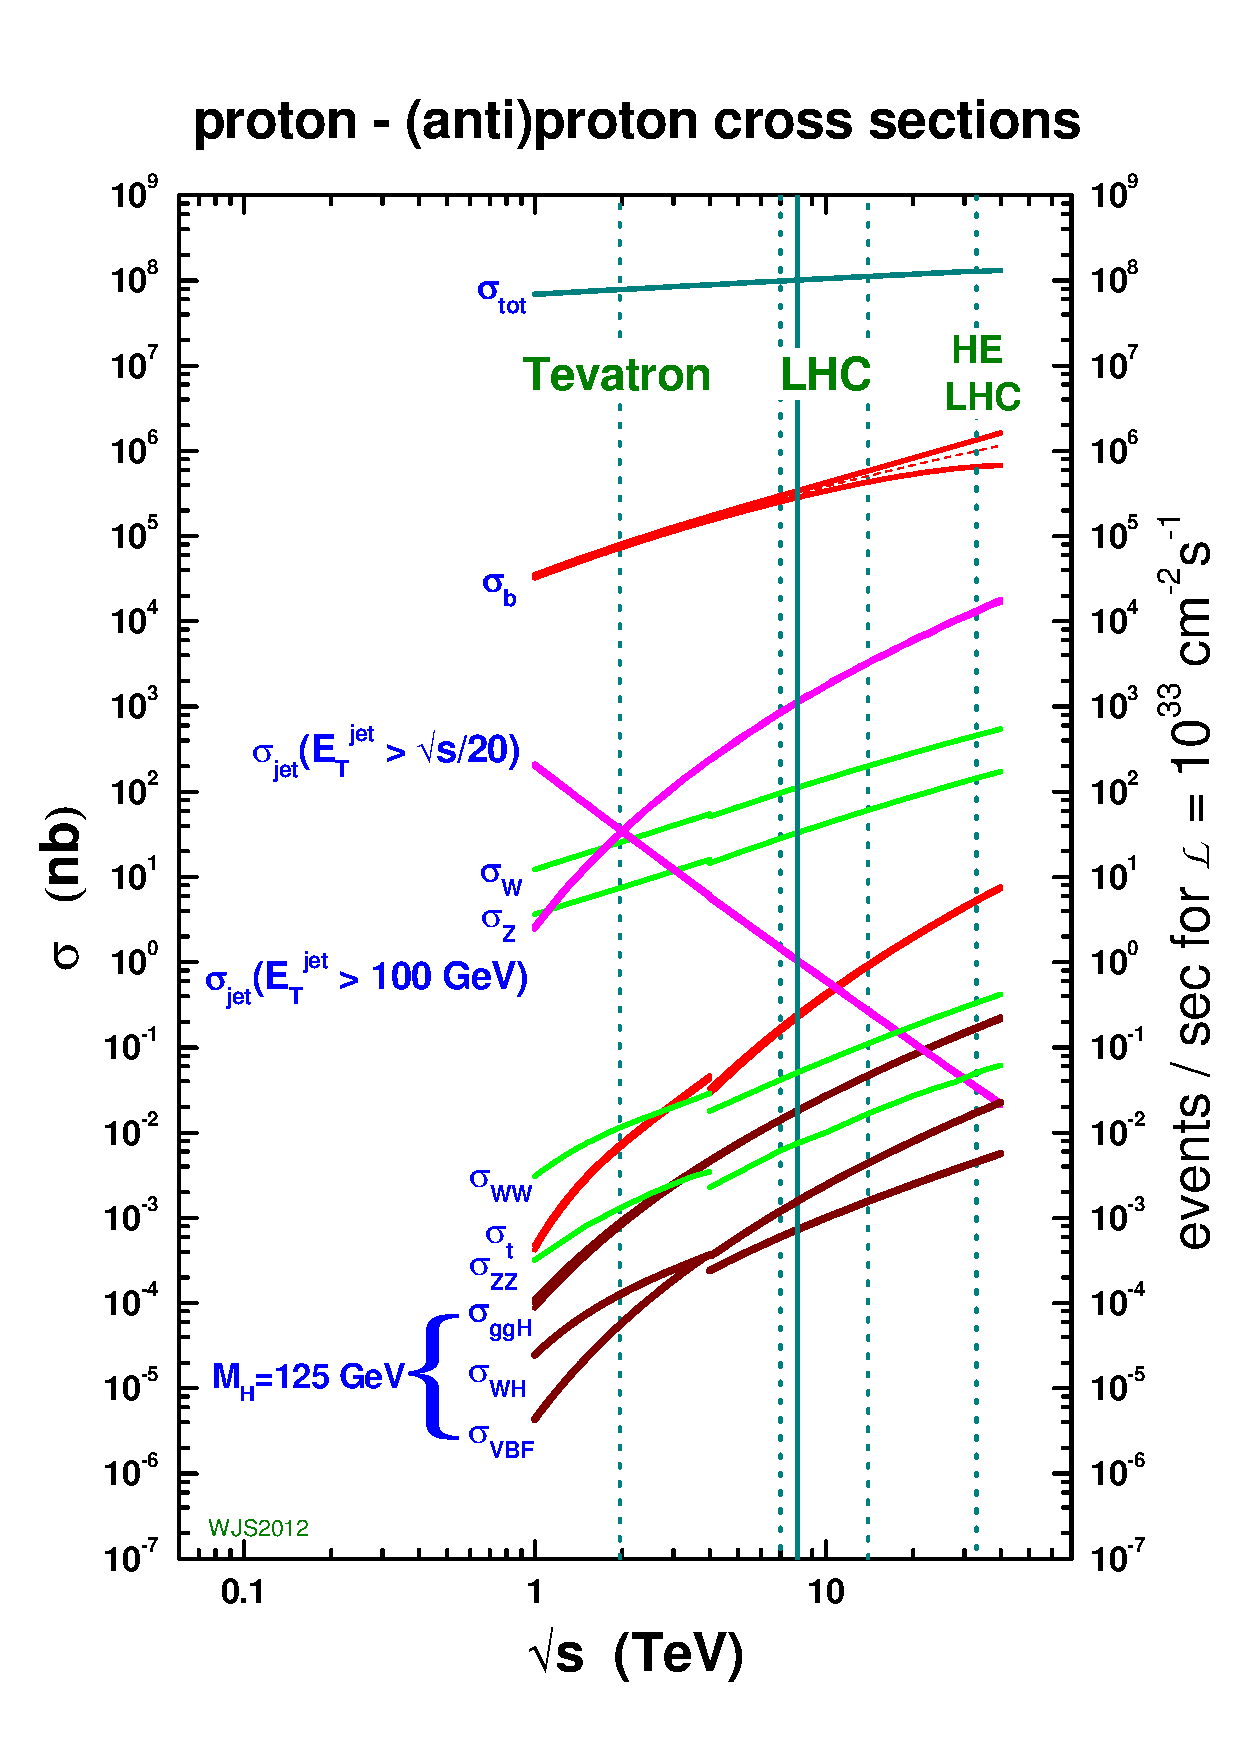
\includegraphics[width=0.6\textwidth]{fig/sm_beyond/crosssections2012HE_v4.pdf}
%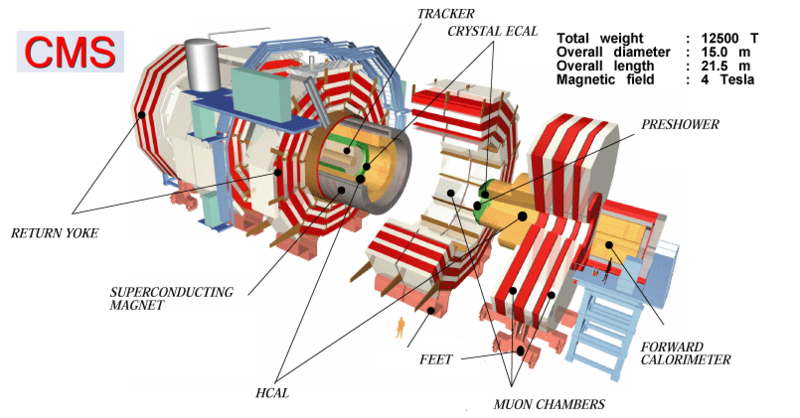
\includegraphics[scale=0.4, trim=20 50 60 30,clip]{fig/chapt3/CMS_exper.png}
\caption{\label{fig:lhclumi_plot}The Standard Model cross sections as a function of energy~\cite{lhclumi_plot}.}
\end{figure}
\subsubsection*{Top quark production}
In hadron colliders, two mechanisms are responsible for the production of top quark – $t\bar{t}$ pairs via strong interaction and single top production via electroweak process, where $t\bar{t}$ is the most abundant production in the high-energy regime. The production of $t\bar{t}$ is contributed by the two LO processes at tree level shown in Fig.~\ref{fig:ttbar_prod}: quark–antiquark ($q\bar{q}$) annihilation and gluon–gluon (gg) fusion in the s-, t-, and u-channel. In $p\bar{p}$ collider such as Tevatron, the dominant production mode for $t\bar{t}$ is the $q\bar{q}$ annihilation while for $pp$ collider like LHC, $gg$ fusion more likely takes place. The hadronic production cross section of the $t\bar{t}$ pair is successfully explained by the QCD and obtained from the proton-proton interaction using the factorization theorem~\cite{ttbar_production} read as:
\begin{equation}
d\sigma_{pp\rightarrow t\bar{t}}(s,m_{t}) = \sum\limits_{i,j=q,\bar{q},g}\int dx_{i}dx_{j}f_{i}(x_{i},\mu^{2}_{f})f_{j}(x_{j},\mu^{2}_{f}).\hat{\sigma}_{ij\rightarrow t\bar{t}}(\hat{s}, m_{t}, \mu_{f},\mu_{r}, \alpha_{s}))
\end{equation}
The cross sections are integrated over all partons participating in the scattering process with momentum fractions x$_i$ and x$_j$ with respect to the proton momenta and summed over all parton types $i$ and $j$. The PDFs $f_{i}(x_{i}, \mu^{2}_{f})$ are partonic distribution functions that describe the probability of finding a parton $i$ inside a hadron in the momentum range x to x+dx. The PDFs absorbs all types of long-distance effects of partons inside the hadrons, whereas the hard scattering partonic cross section $\hat{\sigma}$ represents the actual hard process at small distances that can be computed in perturbative QCD. The long- and short-distance processes can be separated by introducing a new energy scale called the“factorization scale ($\mu_{f}$)” upon which both PDFs and $\hat{\sigma}$ depend. The hard-scattering partonic cross section $\hat{\sigma}$ further depends on the partonic centre-of-mass energy $\hat{s} = x_{i}x_{j}s$ (s is the $pp$ centre-of-mass energy squared), $\mu_{r}$ is the renormalization scale for ultraviolet divergence treatment, and the strong coupling constant $\alpha_{s}$. Both energy scales, $\mu_{f}$ and $\mu_{r}$, are set to the physical energy scale of the process, like for $t\bar{t}$ pair production cross section, they are set to the top quark mass; $\mu_{f} = \mu_{r} = m_{t}$. The recent measurement of $\sigma(t\bar{t})$ at CMS resulted $834.6\pm 2.5 (\text{stat})\pm 19.1 (\text{syst})\pm 22.5 (\text{lumi})\pm 12.5 (\text{extrapol.})$ pb~\cite{CMS-AN-15-233}, in agreement with the SM prediction.
\begin{figure}[h]
\centering
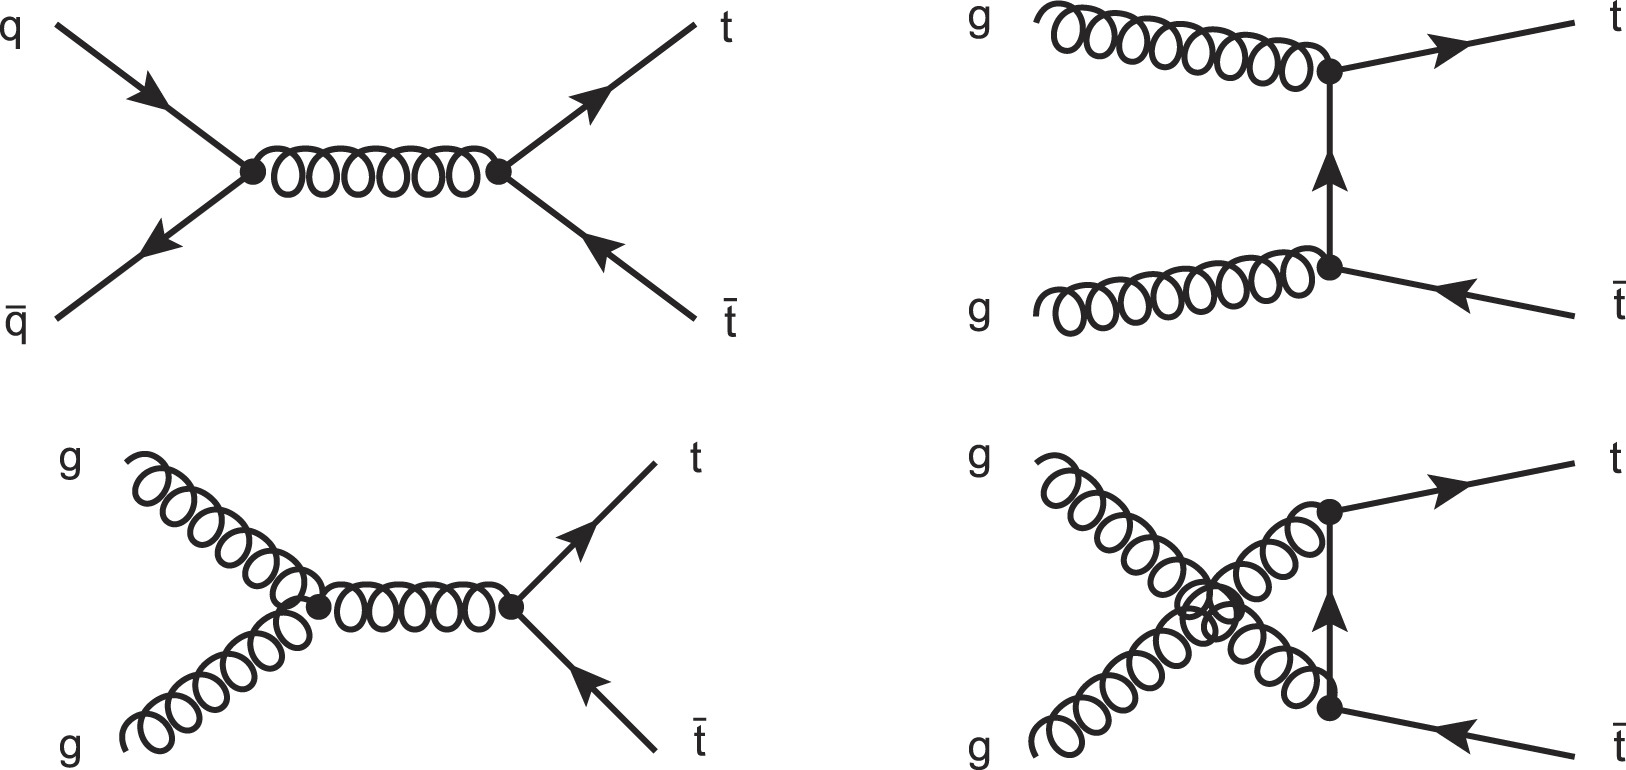
\includegraphics[width=0.7\textwidth]{fig/sm_beyond/ttbar_productions.jpg}
\caption{\label{fig:ttbar_prod}$t\bar{t}$ pair production in QCD at LO: top left is $q\bar{q}$ annihilation, bottom left is gg fusion in the s-channel, top right is gg fusion in the t-channel, and bottom right is gg fusion in the u-channel.}
\end{figure}

Single-top can be produced using hadron colliders through several processes. Among them, three electroweak processes are prominent – t-channel (the dominant channel with 70\% of the total cross section), the associated production of a top (anti-top) quark, a W boson (tW-channel with 25\% cross section), and the s-channel (5\% of the total cross section). The Feynman diagrams for the three processes of single-top quark production are shown in Fig.~\ref{fig:single_top_production}. The electroweak production vertex includes the CKM matrix element V$_{tb}$ that makes the single-top processes more interesting for SM and BSM physics~\cite{Giammanco:2015bxk}.
\begin{figure}
 \centering
 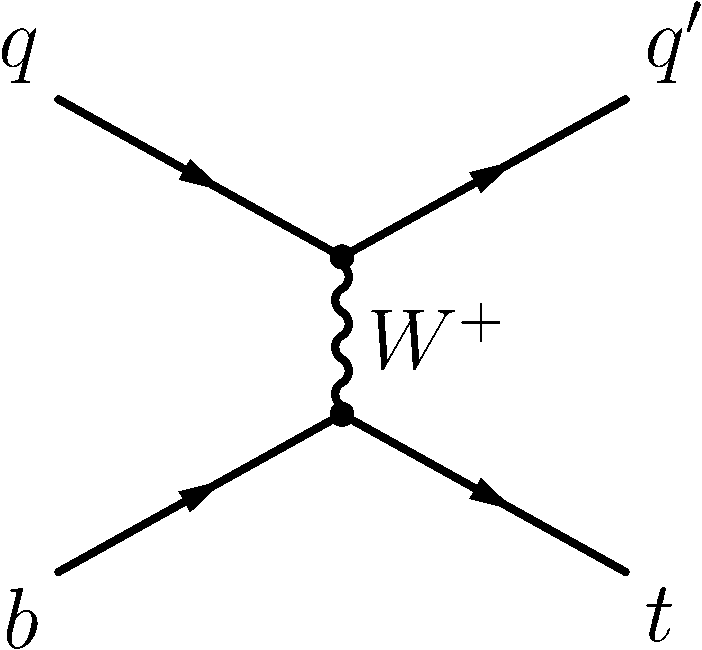
\includegraphics[width=0.25\textwidth]{fig/sm_beyond/tchannel22.pdf}\hfill
 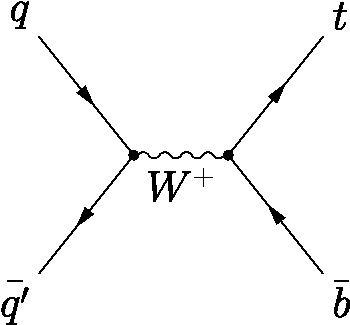
\includegraphics[width=0.25\textwidth]{fig/sm_beyond/s-channel.pdf} \hfill
 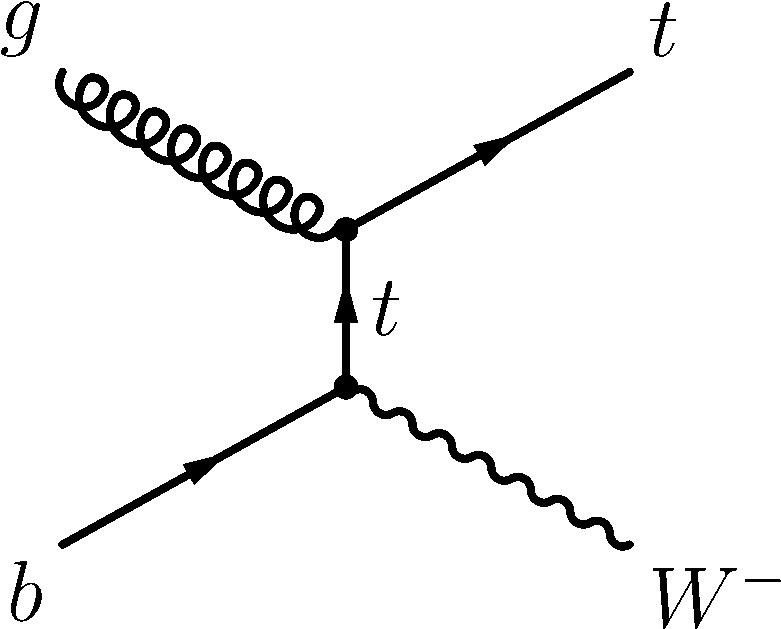
\includegraphics[width=0.25\textwidth]{fig/sm_beyond/WtProduction.pdf}
\caption{Feynman diagram for electroweak single top quark production in the standard model. From left to right: t-channel, s-channel and W-associated production.}\label{fig:single_top_production}
\end{figure}
\subsubsection*{Top quark decay}
The top quark almost exclusively decays into a W boson and a b-quark via electroweak interaction due to the CKM matrix element V$_{tb} \approx$ 1. As compared to other quarks of the SM, top quark has a very short life span ($\tau_{t} \approx 5 \times 10^{-25}$\,s) and decays before hadronization ($\tau_{had} \approx 10^{-24}s$). This makes it more interesting to study the top quark in its bare state along with its kinematic and dynamic information, such as spin correlation transfers to its decay products without being diluted by hadronization. The decay of $t\bar{t}$ system can be classified on the basis of W boson decay products, where the W boson can decay into a pair of light quarks, with BR($W \rightarrow q\bar{q}') \simeq 67\%$, or charged leptons with corresponding neutrinos of the same generation with BR($W \rightarrow l\nu_{l}) \simeq 33\%$. At first order, the possible decay modes of a $t\bar{t}$ event can be grouped into three main categories, as given in Table~\ref{table:ttbar_decay}
\begin{table}[h]%\footnotesize
\centering
     %\begin{tabular}{|p{1.4cm}|p{1.0cm}|p{1.0cm}|}
    \tabulinesep=1.0mm
     \begin{tabu}{|l|c|c|}
        \hline
        Channel & Decay mode & BR\\
\hline 
Hadronic & $t\bar{t}\rightarrow b\bar{b}W^{+}W^{-}\rightarrow b\bar{b}q\bar{q}'q''\bar{q}'''$ & 46\%\\ 
\hline
Semileptonic & $t\bar{t}\rightarrow b\bar{b}W^{+}W^{-}\rightarrow b\bar{b}q\bar{q}'l\nu_{l}$ & 45\%\\ 
\hline
Dileptonic & $t\bar{t}\rightarrow b\bar{b}W^{+}W^{-}\rightarrow b\bar{b}ll'\nu_{l}\nu_{l'}$ & 9\%\\
\hline
\end{tabu}
     \caption{Three categories of $t\bar{t}$ sytem decay with branching ratios\cite{ttbar_decay_ratio}.\label{table:ttbar_decay}}
%\end{center}
\end{table}  

\begin{figure}[htp]
\centering
\begin{tabular}{cc}
\hspace{-0.3cm}
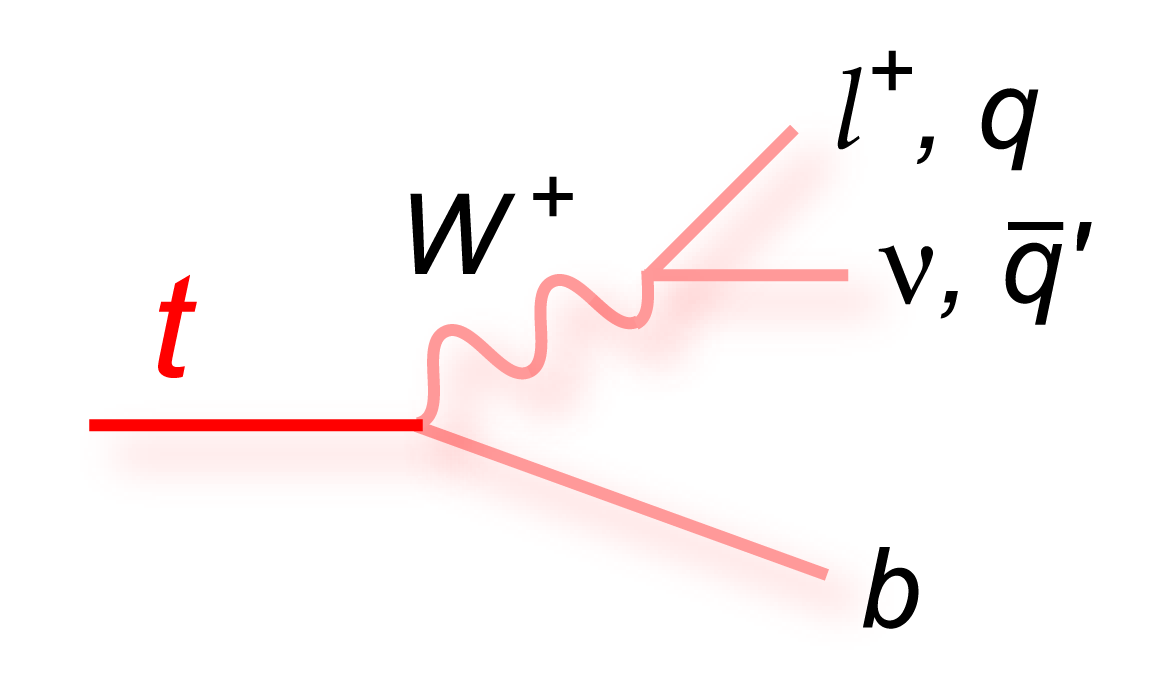
\includegraphics[scale=0.19]{fig/sm_beyond/single_top_decay.png}
& \hspace{-0.5cm} 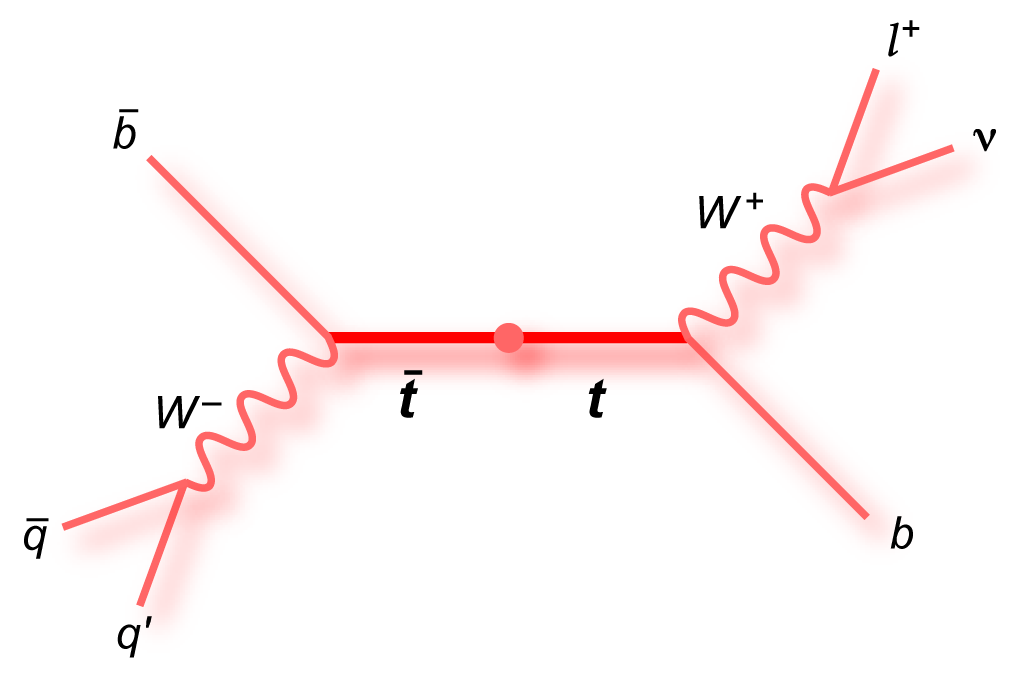
\includegraphics[scale=0.19]{fig/sm_beyond/ttbar_decay.png}\\
   ($\mathbf{a}$)\qquad\qquad\qquad&($\mathbf{b}$)\qquad\\
\end{tabular}
\caption{Feynman diagram for top quark decay (a) and the semileptonic decay of $t\bar{t} $ (b).}\label{fig:top_decay}
\end{figure}
\begin{itemize}
\item {\textbf{Hadronic Channel:}}
Both W bosons coming from $t\bar{t}$ event decay into light quark–antiquark pairs (quark and antiquark further hadronized in the form of jets) with high-branching fraction, resulting in a large sample of selected events. In this channel, at least six jets are required – two of them stem from bjets and remaining from light jets. In hadron colliders like LHC, this channel suffers from an overwhelming QCD multijet background, whose cross section many magnitudes higher than the one for $t\bar{t}$ production. The QCD multijet background is difficult to model from simulation and requires data-driven techniques to estimate using collision data.
\item{\textbf{Dileptonic Channel:}}
In dileptonic channel, both W bosons decay leptonically, resulting two bjets, two charged leptons, and two corresponding neutrinos in $t\bar{t}$ event. It has the lowest branching ratio but a very clean signature at the experimental level due to the presence of two oppositely charged leptons, which can be easily distinguished from QCD multijet events. The disadvantage of a dileptonic event is the presence of two neutrinos, considered as the missing transverse energy in the event, where $t\bar{t}$ can’t be reconstructed perfectly. 
\item{\textbf{Semileptonic Channel:}}
Finally, the lepton+jets channel, whose decay chain is shown in Fig.~\ref{fig:top_decay}b, is a good compromise between a reasonable BR and a relatively clean experimental signature with re-constructible tt-event topology (especially when lepton = $\mu$, e). The semileptonic channel is restricted to $\mu$ + jets and e + jets as the $\tau$ lepton further decay into charged lepton and neutrino or jets that make the channel more complicated. Therefore, a dedicated study is needed to take into account the $\tau$ + jets channel.
 
With a clean signature and adequate BR ($\sim$30\%), the $l(\mu/e)+jets$ channel was chosen for the analysis included in this thesis. In the resolved case, where the final products of each top quark ($p_{T} \le 400$\,GeV) are reconstructed as separate objects, the $t\bar{t}$ final objects consists of four jets, one charged lepton (muon or electron) and neutrino. Two of the jets, tagged as bjets, arise directly from the decay of top quark, while two of the light jets come from one of the W bosons. The second W boson decays into a charged lepton and corresponding neutrino. As the neutrino escapes without detection, it is treated as missing transverse energy ($E^{miss}_{T}$) in the event. The longitudinal component of $E^{miss}_{T}$ is unmeasured and can be reconstructed using the analytical solution explained in detail in~\cite{Betchart:2013nba}. The $t\bar{t}$ system is reconstructed using the Rochester Algorithm explained in Sec.~\ref{subsec:ttbar_reco}.     
\end{itemize}
\subsection{The SM Higgs boson}
In the early 60s, the existence of the Higgs boson was theoretically predicted by Robert Brout, Fran\c cois Englert, and Peter Higgs using the well-known BEH mechanism, as explained in Sec.~\ref{item:higgs_mechanism}. The main goal in the field of particle physics during the last few decades has been the discovery of the Higgs boson, where a number of searches have been conducted at the Large Electron-Positron Collider (LEP) at CERN and at Fermilab with the experiments CDF and D\cancel{0} at $\sqrt{s} = 1.96$\,TeV, using an integrated luminosity of 10.0\,fb$^{-1}$. The mass range was later narrowed down by excluding two regions: 100 < m$_{H}$ < 130\,GeV/c$^{2}$ and 147 < m$_{H}$ < 180\,GeV/c$^{2}$, at the 95\% C.L. Furthermore, they observed a significant access of data events with respect to the background estimation in the mass range, 115 < m$_{H}$ < 140\,GeV/c$^{2}$~\cite{sm_higgs_fermilab}. The official announcement of the Higgs boson discovery, with 5$\sigma$ significance, was made by CERN experiments, CMS, and ATLAS in July 2012 by combining data of 7 and 8\,TeV energy with integrated luminosity of 10.4\,fb$^{-1}$ (CMS) and 10.6\,fb$^{-1}$ (ATLAS)~\cite{cms_sm_higgs,atlas_sm_higgs}. The search was performed in five Higgs decay modes – $\gamma\gamma$, ZZ, W$^{+}$W$^{-}$, $\tau^{+}\tau^{-}$, and $b\bar{b}$, where the excess is most significant in the two decay modes with the best mass resolution, $\gamma\gamma$ and ZZ. By performing a fit to the signals, the mass of the Higgs boson is found to be 125.3$\pm$0.4(stat.)$\pm$0.5(syst.)\,GeV. At 13\,TeV, the study has been repeated and the mass of the Higgs boson was measured to be 124.50$^{+0.48}_{-0.46}$\,GeV with a constraint on the width $\Gamma_{H}$ < 41\,MeV~\cite{sm_higgs_13tev}. The measured cross section agrees well with the expectation of the SM. The signal strength $\mu$, defined as the production cross section of the Higgs boson times its branching fraction to four leptons relative to the SM expectation, is measured as $\mu$ = 0.99$^{+0.33}_{-0.26}$ at m$_{H}$ = 125.09\,GeV. The properties of the Higgs boson, such as spin, parity, ratios of production rates for different production modes, ratios of couplings to fermions and vector bosons, etc. agree well with the SM prediction. The Higgs mass measured at 13\,TeV using 12.9\,fb$^{-1}$ data in two channels $H\rightarrow\gamma\gamma$ (a) and $H\rightarrow ZZ\rightarrow 4l$ (b) is shown in Fig.~\ref{fig:sm_higgs}, where the excess around 125\,GeV in the data is visible. 
   
\begin{figure}[htp]
\centering
\begin{tabular}{cc}
\hspace{-0.3cm}
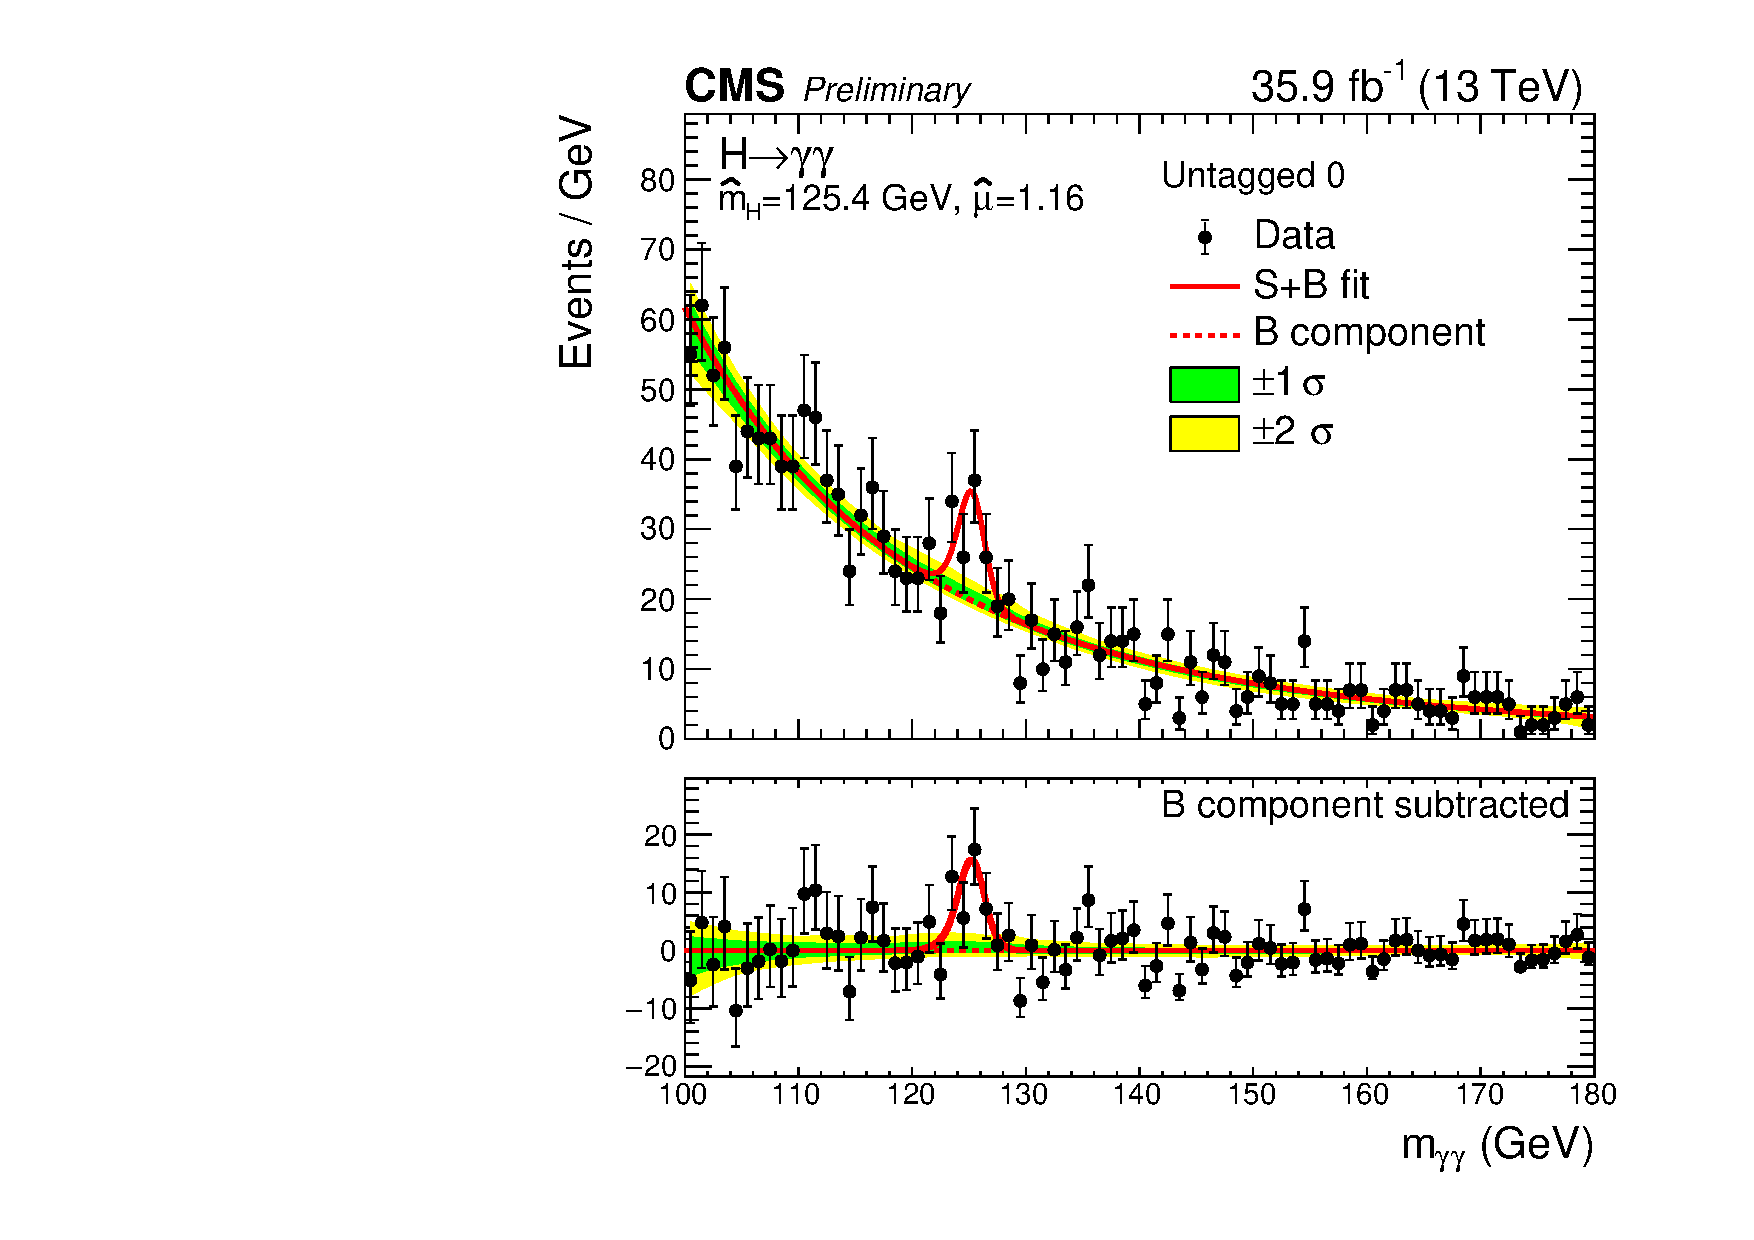
\includegraphics[scale=0.35]{fig/sm_beyond/CMS-PAS-Htogamma.pdf}
& \hspace{-0.5cm} 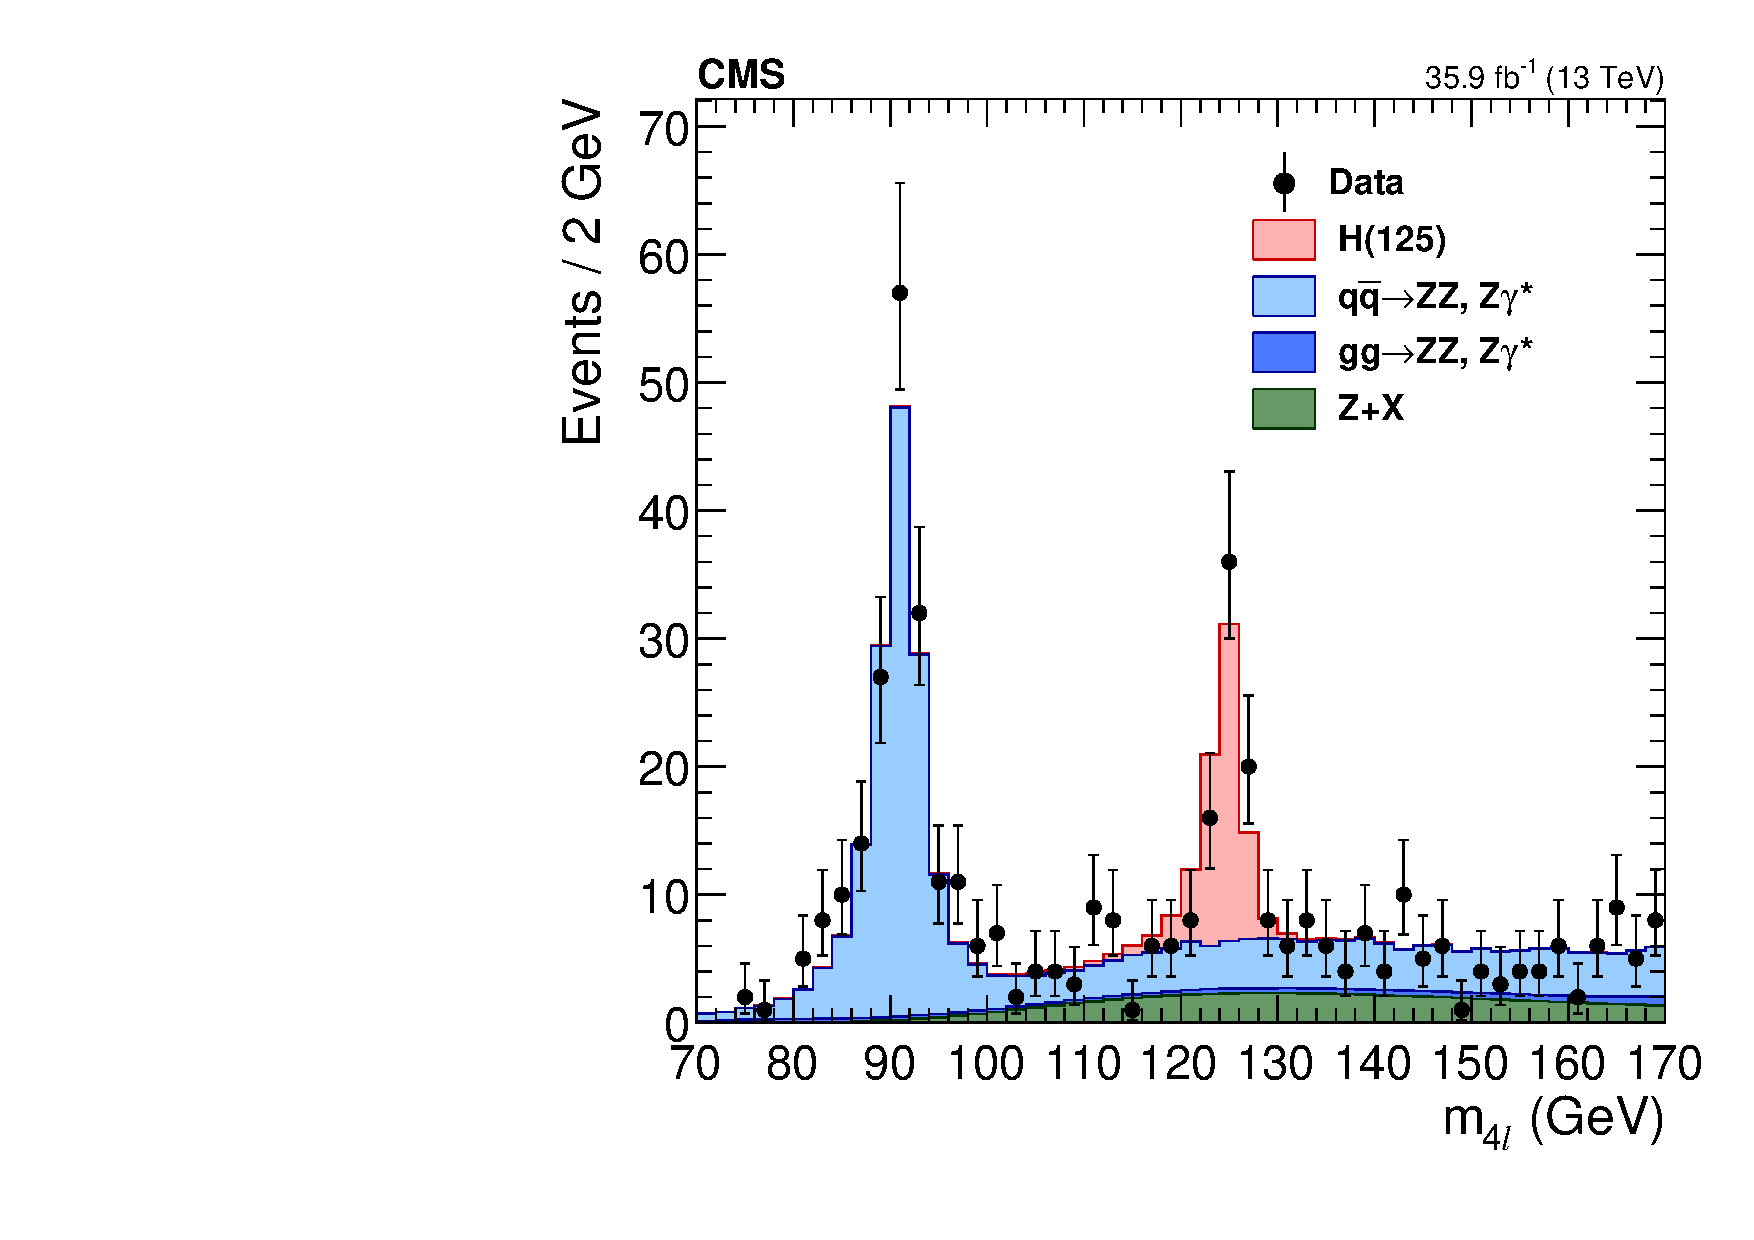
\includegraphics[scale=0.35]{fig/sm_beyond/CMS-PAS-Hto4l.pdf}\\
   ($\mathbf{a}$)\qquad&($\mathbf{b}$)\qquad\\
\end{tabular}
\caption{\label{fig:sm_higgs}The SM Higgs mass spectra obtained in the 2016 CMS search using the two most sensitive decay channels, di-photon (left) and four-lepton (right). Both channels show more than 5 standard deviations significance of the observed signals around 125\,GeV; the data corresponds to an integrated luminosity of 13\,fb$^{-1}$, collected with the CMS detector at a centre-of-mass energy of 13\,TeV~\cite{pub:sm_higgs4l,pub:sm_higgs2gamma}.}
\end{figure} 

\begin{itemize}
\item{\textbf{Production and decay of the SM Higgs boson:}} The SM Higgs boson couples with every massive particle; hence, the production in hadron collider is possible in many ways. The following four are the most common.
\begin{enumerate}
\item{\textbf{Gluon-gluon fusion (ggF):}} In this mode of production, two gluons interact to produce a Higgs boson mediated by heavy quarks (mainly top quark) loop as Higgs boson doesn't directly couple to massless gluon. This channel of production has a higher cross section throughout the Higgs boson mass range.
\item{\textbf{Vector boson fusion (VBF):}} In the VBF mode, two quarks from colliding protons radiate massive vector bosons (W or Z) and its fusion results in the production of the Higgs boson. It is the second highest cross section process with 10 times less than the ggH but has a clear signature because of the pure electroweak process. 
\item{\textbf{Associated production with W$^{\pm}$ or Z$^{0}$ (VH):}} This process is also known as Higgs-Strahlung, the third highest cross section, in which a massive vector boson is produced by the interaction of a valence quark with an antiquark from the sea and the massive vector boson further radiates a Higgs boson. This mode is helpful for testing the Higgs coupling with the massive vector boson.
\item{\textbf{Associated production with $t\bar{t}$ ($t\bar{t}$H):}} In this mode of production, the Higgs is associated with heavy quark pairs, like the top quark pair, which can be initiated either by gluon-gluon fusion or $q\bar{q}$ annihilation. This channel has smaller cross sections but is more interesting because of the direct coupling with the top quark.
\end{enumerate} 
Higgs boson decays through many channels, either through direct coupling to the final state massive particles or indirectly via a boson or fermion loop in massless final state particles (photon, gluon). The decay channel $H\rightarrow b\bar{b}$ has the largest branching ratio (BR) but is diluted by the irreducible QCD background which mimics the signal. The same is true for the $H\rightarrow \tau\bar{\tau}$ channel, where $\tau$ decays hadronically. Despite the low BRs, the two channels $H\rightarrow ZZ^{\star}\rightarrow 4l$ and $H\rightarrow \gamma\gamma$ show a very clear signature to the Higgs. Ultimately, the Higgs discovery became possible owing to these two channels. Figure~\ref{fig:sm_higgsxsec_BR} (a) shows the Higgs cross section as a function of centre-of-mass energy for m$_{H}$ = 125\,GeV with a band of theoretical uncertainty and (b) shows the BRs as a function of Higgs mass with a band of total uncertainty(\%).     
\end{itemize} 
\begin{figure}[htp]
\centering
\begin{tabular}{cc}
\hspace{-0.3cm}
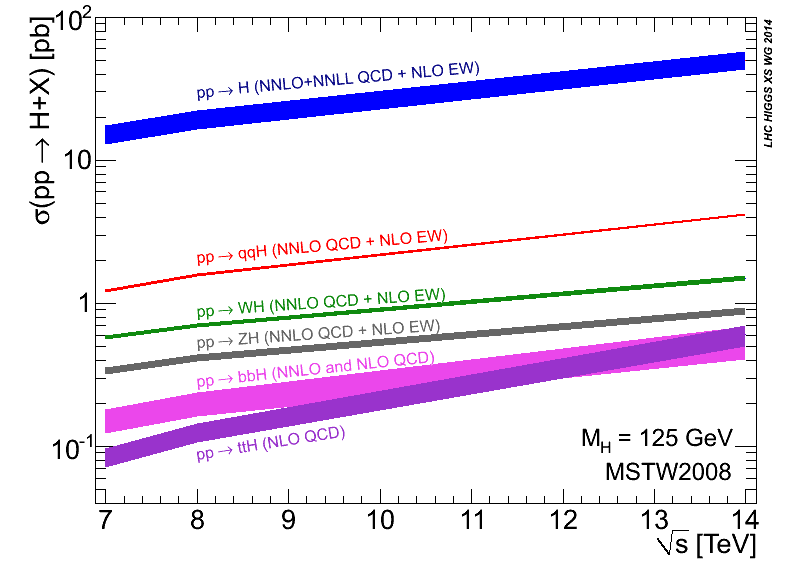
\includegraphics[scale=0.278]{fig/sm_beyond/7_14_xsec.png}
& \hspace{-0.5cm} 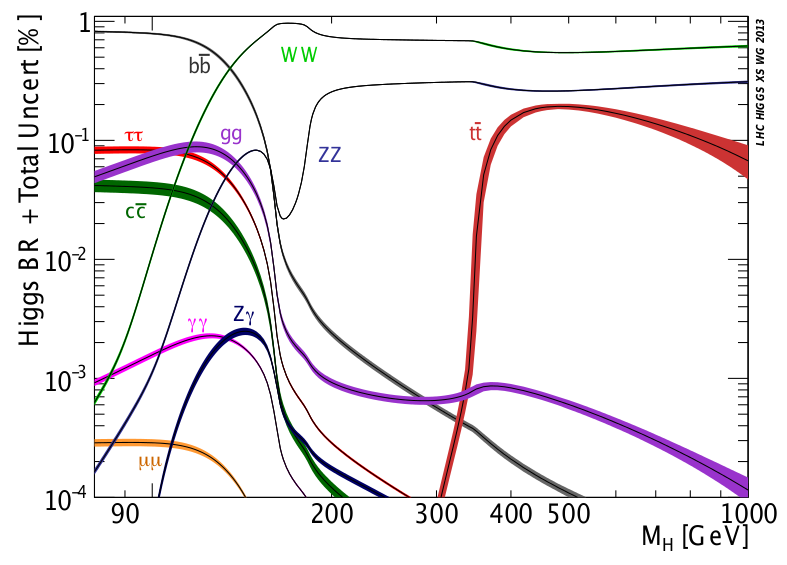
\includegraphics[scale=0.38]{fig/sm_beyond/Higgs_BR_RECT.png}\\
   ($\mathbf{a}$)\qquad&($\mathbf{b}$)\qquad\\
\end{tabular}
\caption{\label{fig:sm_higgsxsec_BR} Higgs boson (a) production cross section for main modes as a function of centre-of-mass energy exploiting m$_{H}$ = 125\,GeV for $pp$ collider and (b) branching ratio (BR) with full uncertainty in almost all channels as a function of Higgs mass~\cite{pub:sm_higgsxsec}.}
\end{figure} 
\section{Beyond the Standard Model}\label{sec:bsm}
Although the SM has been tested with great success with regard to predicting and explaining many physics processes, especially in its gauge and flavour sector, it is still not the ultimate theory. This is because there exist a few experimental pieces of evidence and theoretical issues that are not explained by the SM. The most prominent among them are gravity, matter–anti-matter asymmetry, existence of dark matter and dark energy, and non-vanishing neutrino mass. There are some fundamental characteristics of the SM that we can't explain. The most important among them are: Why is the mass of the SM Higgs boson 125\,GeV when the Planck scale is $\mathcal{O}(10^{19})$\,GeV? This phenomenon is commonly known as the Hierarchy Problem and is a basic motivation for this search, as explained in more detail in Sec.~\ref{subsec:hierarchy}. Similarly, another question that arises is: Why do we have three families of fermion that have a wide mass range?
\subsection{The Hierarchy problem}\label{subsec:hierarchy}
Physics beyond the Standard Model (SM) can be probed for many reasons, but the core issue before us today, which is relevant to Higgs boson physics and electroweak explorations at the Large Hadron Collider, is the Hierarchy Problem. The problem involves the large difference between the Planck mass $M_{pl} \approx 10^{19}$\,GeV, an energy scale associated with gravity, and the electroweak symmetry breaking scale ($10^{2}$) of the SM. Higgs boson is the only fundamental scalar in the SM that can be subjected to higher-order loop corrections from spin 0, 1/2, and 1 particle with a quadratic dependence on the cut-off scale (Planck scale). These corrections may take the Higgs mass to the highest scale, but the Higgs mass $\sim$ 125\,GeV is in contrast. The masses of fermions and gauge bosons are protected by chiral and local gauge symmetry respectively, but for scalar Higgs, there is no symmetry banning its mass term $m^{2}H^{\dagger}H$. In Fig.~\ref{fig:higgs_massloop}, the upper row shows the quantum loop corrections to the Higgs mass; left is the Higgs self-interaction, middle is the gauge boson loop, and right shows the fermionic loop. In mathematical language, consider massive $N_{f}$ fermions with Youkawa coupling $\lambda = \sqrt{2}m_{f}/\nu$. Neglecting the external Higgs momentum squared, we obtain:
\begin{equation}\label{equ:hierarchy}
\Delta M_{H}^{2} = N_{f}\frac{\lambda_{f}}{8\pi^{2}}\Big[\Lambda^{2} + 6m_{f}^{2}log\frac{\Lambda}{m_{f}} - 2m_{f}^{2} \Big] + \mathcal{O}(\frac{1}{\Lambda^{2}})
\end{equation}
Where $\Delta M_{H}^{2}\propto \Lambda^{2}$. If we consider the cut-off scale to be the Planck scale $M_{pl} \approx 10^{19}$\,GeV, the Higgs boson mass becomes very huge, which stands against the experimental results. A counter-term $\mathcal{O}(10^{-30})$ needs to be added to the mass squared so that the value matches with the experimental result, but this seems unnatural. This is commonly known as fine-tuning or naturalness~\cite{hierarchy}. Several theories are proposed to cancel out infinities and leave the mass around the Higgs mass (125\,GeV). Supersymmetry (SUSY) is one of the leading possibilities for solving the naturalness and Hierarchy Problem by introducing ``superpartner'' to the SM Higgs particles. Such superpartners introduce additional Feynman diagrams to cancel out the infinities, as shown in the lower row in Fig.~\ref{fig:higgs_massloop} for Higgs, W boson, and top quark.     
\begin{figure}[htp]
\centering
\hspace{-0.3cm}
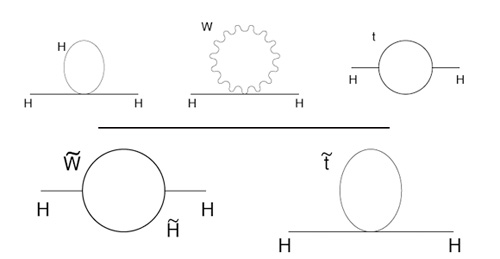
\includegraphics[scale=0.65]{fig/sm_beyond/higgs_mass_loop.jpg}
\caption{\label{fig:higgs_massloop}The three Feynman diagrams in the top row, from left to right, represent Higgs self-, W/Z boson, and fermion (top quark) coupling respectively – a quantum effects on the Higgs mass. These effects boost the Higgs mass to an infinite value that needs to be finite by using some unknown contributions. SUSY suggests supersymmetric partners of the SM particles, one must include additional diagrams, where superpartners cancel out the effects of the loops in the Higgs mass calculation, as shown in the lower row. Source of the Feynman diagrams is~\cite{pub:higgsmassloop}.}
\end{figure}

\subsection{Supersymmetry}
Supersymmetry (SUSY) is a space-time symmetry relating to two different classes of particles – integer spin-0 and spin-1 (bosons) and spin-1/2 (fermions)~\cite{phd_thesis:susy}. The SUSY generators $\mathcal{Q}$ transform a fermionic state into a bosonic state and vice-versa:
\begin{equation}\label{equ:susy_gen}
\mathcal{Q}|Fermion\rangle = |Boson\rangle, \mathcal{Q}|Boson\rangle = |Fermion\rangle
\end{equation}
When the symmetry is exact, bosons and fermions have the same mass and quantum number, except for the spin. But the question arises, why didn’t we find superpartners of the SM particles? For example, the electron was discovered more than a century ago. If it has a superpartner with the same mass and charge with opposite spin, it should be discoverable through simple experiments. Similarly, no squark (where ``s’’ stands for superpartner) has been observed in hadron-hadron colliders so far. This suggests that SUSY does not have exact symmetry and must be broken in a manner such that the superpartners acquire higher masses (higher than the top quark) but not too high as to reintroduce the Hierarchy Problem. This is commonly known as the ``soft’’ breaking of the SUSY. Up till now, nobody has found a completely satisfactory dynamic way to break SUSY; however, there are many optional cases, where the SUSY can break. One possibility is to introduce the soft term to the SUSY Lagrangian by hand, which breaks the SUSY explicitly. 
\begin{equation}\label{equ:soft_break}
\mathcal{L} = \mathcal{L}_{SUSY} + \mathcal{L}_{soft}
\end{equation}
This results in a low-energy effective SUSY theory and can be used for mass and decay predictions. Minimal Supersymmetric Standard Model (MSSM) is the most economical version that will be discussed in detail in the next section~\ref{subsec:mssm}.   
\subsection{Minimal Supersymmetric Standard Model}\label{subsec:mssm}
The Minimal Supersymmetric Standard Model (MSSM)~\cite{Martin:1997ns} is based on the group $\text{SU}(3)_{C}\times \text{SU}(2)_{L}\times \text{U}(1)_{Y}$ with a minimal amount of additional fields required with regard to the existing one in order to make the theory supersymmetric. In MSSM, each SM particle has its superpartner differ by spin–1/2. An overview of the gauge bosons (spin-1) and their spin–1/2 partners, the gauginos, is given in Table~\ref{table:mssmgauge}. 
\begin{table}[h]%\footnotesize
\centering
     %\begin{tabular}{|p{1.4cm}|p{1.0cm}|p{1.0cm}|}
    \tabulinesep=1.0mm
     \begin{tabu}{|l|c|c|c|c|}
        \hline
        Names & Superfield $\widetilde{S}$ & Spin-$\frac{1}{2}$ & Spin-1 & $SU(3)_{C}$, $SU(2)_{L}$, $U(1)_{Y}$ \\
\hline 
gluino, gluon & $\hat{G}^{a}$ & $\widetilde{G}$ & g & (8, 1, 0) \\ 
\hline
winos, W bosons & $\hat{W}$ & $\widetilde{W}^{\pm}, \quad \widetilde{W}^{0}$ & $W^{\pm}, \quad W^{0}$ & (1, 3, 0) \\ 
\hline
bino, B boson & $\hat{B}$ & $\widetilde{B}^{0}$ & $B^{0}$ & (1, 1, 0) \\
\hline
\end{tabu}
     \caption{Gauge supermultiplets in the MSSM with quantum numbers.\label{table:mssmgauge}}
%\end{center}
\end{table}  
In SM, there are three generations of spin–1/2 fermions (quarks and leptons without right-handed neutrino) that correspond to spin-0 SUSY superpartners, squarks, and sleptons: $\hat{Q}, \hat{U}_{R}, \hat{D}_{R}, \hat{L}, \hat{E}_{R}$. SUSY requires two Higgs doublets for anomaly cancellation and to give mass to all fermions. Conventionally, the two Higgs doublets are denoted by $H_{u}$ with Y = +1/2 and $H_{d}$ with Y = -1/2, where the first one gives mass to the up-type quarks and the second to the down-type and charged leptons. Table~\ref{table:mssmparticles} summarizes the particles and their supermultiplets.

Unlike the SM, SUSY doesn’t respect lepton and baryon number conservation. This can be enforced in a simple manner – by introducing a discrete and multiplicative symmetry called R–parity: 
\begin{equation}\label{equ:rparity}
R_{p} = (-1)^{2s+3B+L}
\end{equation}
Where s, B, and L represent spin, baryon, and lepton number respectively. For the ordinary particles (fermions, gauge bosons, and Higgs bosons), $R_{p}$ = +1 and for their superpartner $R_{p}$ = -1. SUSY allows $R_{p}$ conservative terms in its Lagrangian. In practice, R-parity conservation has important effects on the MSSM phenomenology by allowing pair production of the SUSY particles in colliders. Further decay of the SUSY particles comprises an odd number of SUSY particles, where the stable lightest supersymmetric particle (LSP) is a strong candidate for dark matter if it is neutral and only weakly interacting.    
\begin{table}[h]%\footnotesize
\centering
     %\begin{tabular}{|p{1.4cm}|p{1.0cm}|p{1.0cm}|}
    \tabulinesep=1.0mm
     \begin{tabu}{|l|c|c|c|c|}
        \hline
        Names & Superfield $\widetilde{S}$ & Spin-0 & Spin-$\frac{1}{2}$ & $SU(3)_{C}$, $SU(2)_{L}$, $U(1)_{Y}$ \\
\hline 
squarks, quarks & $\hat{Q}$ & ($\widetilde{u}_{L} \quad \widetilde{d}_{L}$) & ($u_{L} \quad d_{L}$) & (3, 2, $\frac{1}{6}$) \\ 
 
($\times$ 3 families) & $\hat{U}$ & $\widetilde{u}_{R}^{\star}$ & ${u}^{\dagger}_{R}$ & ($\overline{3}$, 1, $-\frac{2}{3}$) \\

                      & $\hat{D}$ & $\widetilde{d}_{R}^{\star}$ & ${d}^{\dagger}_{R}$ & ($\overline{3}$, 1, $\frac{1}{3}$) \\
\hline
sleptons, leptons & $\hat{L}$ & ($\widetilde{\nu} \quad \widetilde{e}_{L}$) & ($\nu \quad e_{L}$) & (1, 2, $-\frac{1}{2}$) \\ 

($\times$ 3 families) & $\hat{E}$ & $\widetilde{e}_{R}^{\star}$ & ${e}^{\dagger}_{R}$ & (1, 1, 1) \\
\hline
Higgs, Higgsinos & $\hat{H}_{u}$ & ($H^{+}_{u} \quad H^{0}_{u}$) & ($\widetilde{H}^{+}_{u} \quad \widetilde{H}^{0}_{u}$) & (1, 2, $+\frac{1}{2}$) \\
                 & $\hat{H}_{d}$ & ($H^{0}_{d} \quad H^{-}_{d}$) & ($\widetilde{H}^{0}_{d} \quad \widetilde{H}^{-}_{d}$) & (1, 2, $-\frac{1}{2}$) \\
\hline
\end{tabu}
     \caption{Chiral supermultiplets in the MSSM with quantum numbers.\label{table:mssmparticles}}
%\end{center}
\end{table}  
In light of the above-mentioned properties, it is easy to define a globally supersymmetric Lagrangian for MSSM. I will only discuss the final results here, without going into detail about the derivation because it is beyond the scope of this thesis. The kinetic part of the Lagrangian is the supersymmetric equivalent of the SM and is obtained by generalizing the notion of covariant derivative to the SUSY. The gauge invariant’s general superpotential, also compatible with renormalizability and R–parity conservation rule, is written as:
\begin{equation}\label{equ:mssmpotential}
W = \sum_{i,j=gen}-Y_{ij}^{u}\hat{u}_{Ri}\hat{H}_{2}.\hat{Q}_{j} + Y_{ij}^{d}\hat{d}_{Ri}\hat{H}_{1}.\hat{Q}_{j} + Y_{ij}^{l}\hat{l}_{Ri}\hat{H}_{1}.\hat{L}_{j} + \mu \hat{H}_{2}.\hat{H}_{1}
\end{equation}
Where i and j run over three generations and $\epsilon_{12}=-\epsilon_{21}=1$ and $\epsilon_{11}=-\epsilon_{22}=0$. $H . Q \equiv \epsilon_{12}H^{1}Q^{2}$ is the SU(2) doublets products and $Y_{ij}^{u,d,l}$ represents the Youkawa couplings among generations. The last term represents a globally supersymmetric mass term for the Higgs doublets.
\subsection{Higgs sector of MSSM}\label{subsec:higgsmssm}
SUSY requires two Higgs doublets for anomaly cancellation and giving mass to all the fermions. This minimal version of SUSY is commonly referred to as the Two Higgs Doublets Model (2HDM). The SM fermions cancel the anomaly by themselves, where the superpartner of the Higgs boson is a fermion that contributes to triangle gauge anomalies. The anomaly can be cancelled out by introducing a second fermion that is basically the vector compliment of the first one. Therefore, MSSM introduces $H_{u}$ and its vector compliment $H_{d}$~\cite{Wells:2009kq}. Similarly, $\hat{H}_{u}$ gives mass to up-type quarks and is unable to give mass to down-type quarks, as in superpotential $\hat{H}_{u}^{*}$ is forbidden and $\hat{H}_{d}$ gives mass to the down-type quarks. The Higgs doublets can be represented in terms of complex field:
\begin{equation}\label{equ:HuHd}
H_{u} = \left(\begin{array}{c}
H^{+}_{u}\\
H^{0}_{u}
\end{array}\right) \quad \textnormal{and} \quad
H_{d} = \left(\begin{array}{c}
H^{0}_{d}\\
H^{-}_{d}
\end{array}\right) 
\end{equation} 
We have not observed the supersymmetric partners of SM particles, which requires the SUSY to be broken at some higher scale. Soft-SUSY breaking mechanism does this job by introducing new terms to the Lagrangian in a manner such that it does not reintroduce quadratic sensitivities to the cut-off. The possibly soft-SUSY terms in the Higgs sector are:
\begin{equation}\label{equ:softsusyHiggs}
\mathcal{V}_{1} = m^{2}_{H_{u}} \left( \abs{H^{+}_{u}}^{2} + \abs{H^{0}_{u}}^{2} \right) + 
m^{2}_{H_{d}} \left( \abs{H^{-}_{d}}^{2} + \abs{H^{0}_{d}}^{2} \right) + 
\left\{ b\left(H^{+}_{u}H^{-}_{d} - H^{0}_{u}H^{0}_{d}\right) + h.c  \right\}
\end{equation} 
Where the parameters $m^{2}_{H_{u}}$, $m^{2}_{H_{d}}$ and b are still arbitrary. The total scalar potential is written as~\cite{phd_thesis:mssm}:
\begin{equation}
\begin{split}
\mathcal{V} = \left(\abs{\mu}^{2} + m^{2}_{H_{u}}\right) \left( \abs{H^{+}_{u}}^{2} + \abs{H^{0}_{u}}^{2} \right)
+\left(\abs{\mu}^{2} + m^{2}_{H_{d}}\right) \left( \abs{H^{-}_{d}}^{2} + \abs{H^{0}_{d}}^{2} \right)\\
+ \left\{ b\left(H^{+}_{u}H^{-}_{d} - H^{0}_{u}H^{0}_{d}\right) + h.c  \right\} +
\frac{g^{2}}{2}\abs{H^{+*}_{u}H^{0}_{d} + H^{0*}_{u}H^{-}_{d}}^{2}\\
+\frac{g^{2}+g'^{2}}{8}\left( \abs{H^{+}_{u}}^{2} + \abs{H^{0}_{u}}^{2} -  \abs{H^{-}_{d}}^{2} - \abs{H^{0}_{d}}^{2}\right)
\end{split}\label{equ:totallagmssm}
\end{equation}
The Higgs mechanism in MSSM can be used to obtain the minimum of this scalar potential in the same way as in SM, where the electromagnetism gauge group U(1) is not broken. We have freedom to suppose a vanishing vev for the electromagnetic part $\big \langle H_{u}^{+} \big \rangle = 0$, at the minimum of the potential, where $\left.\frac{\partial \mathcal{V}}{\partial H^{+}_{u}}\right|_{H_{u}^{+}=0} \Rightarrow H_{d}^{-} = 0$. In the same manner, we consider $\big \langle H_{u}^{-} \big \rangle = 0, \Rightarrow H_{d}^{+} = 0$. Thus, electromagnetism is unbroken, as the charged directions cannot attain a vacuum expectation value. Consider the vev of the neutral part $\big \langle H_{u}^{0} \big \rangle = v_{u}$ and $\big \langle H_{d}^{0} \big \rangle = v_{d}$, hence at minimum of $\mathcal{V}$ we obtain:
\begin{equation}
\begin{split}
\left(\abs{\mu}^{2} + m^{2}_{H_{u}}\right)v_{u} = bv_{d} + \frac{g^{2}+g'^{2}}{4}v_{u}\left(v_{d}^{2} - v_{u}^{2}\right)\\
\left(\abs{\mu}^{2} + m^{2}_{H_{d}}\right)v_{d} = bv_{u} - \frac{g^{2}+g'^{2}}{4}v_{d}\left(v_{d}^{2} - v_{u}^{2}\right)\\
\end{split}
\end{equation}
Where the vevs are related to W/Z masses. Consider the kinetic terms for the Higgs field:
\begin{equation}
\mathcal{L}_{kin} = \left(D_{\mu}H_{u}\right)^{\dagger} + \left(D^{\mu}H_{u}\right) + \left(D_{\mu}H_{d}\right)^{\dagger} + \left(D^{\mu}H_{d}\right)
\end{equation}
with $D_{\mu} = \partial_{\mu} + ig\tau_{a}W_{\mu}^{a}/2 + ig'yB_{\mu}/2$, the W/Z masses can be written as:
\begin{equation}
\begin{split}
m_{W}^{2} = \frac{g^{2}}{2}\left(v_{u}^{2} + v_{d}^{2}\right)\\
m_{Z}^{2} = \frac{g^{2}+g'^{2}}{2}\left(v_{u}^{2} + v_{d}^{2}\right)
\end{split}\label{equ:w_zmass_mssm}
\end{equation}
The two Higgs-doublets extension of the MSSM generates eight scalar degrees of freedom (DoF) before electroweak symmetry breaking (EWSB). After symmetry breaking, three of them are eaten by gauge bosons, given by~\ref{equ:w_zmass_mssm}, and the remaining five DoFs should manifest as physical states. Among five, two of the DoFs are charged ($H^{\pm}$), one is neutral pseudo scalar ($A^{0}$), and two are neutral $\mathcal{CP}$-even scalar $h^{0}$ and $H^{0}$ states, where conventionally $h^{0}$ < $H^{0}$. Their masses can be computed by expanding the doublet fields around their vev $\left( H = \langle H \rangle + \phi + i\varphi \right)$ value and plug this expansion into the Higgs potential. It can be seen that the mass terms of the fields $\varphi_{u}$ and $\varphi_{d}$ only mix among themselves. Taking the ratio of vevs of the doublets as $\tan\beta = \frac{v_{u}}{v_{d}}$, we obtain the $\mathcal{CP}$-odd state $A^{0}$:
\begin{equation}
A^{0} = \sqrt{2}\left(\varphi_{u} \cos\beta + \varphi_{d} \sin\beta \right); \quad m^{2}_{A^{0}} = \frac{b}{sin2\beta}
\end{equation}
For $\phi_{u}$ and $\phi_{d}$ we obtain in the same manner the mass terms:
\begin{equation}
\begin{split}
m_{h^{0}}^{2} = \frac{1}{2}\left[ \left(m_{A^{0}}^{2} + m_{Z}^{2} \right) - \sqrt{(m_{A^{0}}^{2} + m_{Z}^{2})^{2} -4m_{A^{0}}^{2}m_{Z}^{2}\cos^{2}2\beta}\right]\\
m_{H^{0}}^{2} = \frac{1}{2}\left[ \left(m_{A^{0}}^{2} + m_{Z}^{2} \right) + \sqrt{(m_{A^{0}}^{2} + m_{Z}^{2})^{2} -4m_{A^{0}}^{2}m_{Z}^{2}\cos^{2}2\beta}\right]
\end{split}\label{higgs_masses_mssm}
\end{equation}
Consider the possibility that $m_{A^{0}} \gg m_{Z}$, then the mass of the lightest Higgs $h^{0}$ is bounded above by $m_{Z}\abs{\cos2\beta}$. One can include higher-order corrections and large log resummations that push the Higgs mass to $\approx$130\,GeV and expected to behave like SM Higgs boson for most of the MSSM parameter space. The discovery of the SM Higgs boson with mass $\approx$125\,GeV is consistent with these predictions. The corresponding fields for $h^{0}$ and $H^{0}$ are:
\begin{equation}
\begin{split}
h^{0} = \sqrt{2}\left(\phi_{u} \cos\alpha - \phi_{d} \sin\alpha \right)\\
H^{0} = \sqrt{2}\left(\phi_{u} \sin\alpha + \phi_{d} \cos\alpha \right)
\end{split}
\end{equation} 
The charged Higgs field is: 
\begin{equation}
H^{\pm} = \phi^{\pm}_{d}\sin\beta + \phi^{\pm}_{u}\cos\beta
\end{equation}
We can also obtain the equation:
\begin{equation}\label{equ:mixing_ang}
\tan\alpha = -\frac{\left[\frac{1}{2}\left(m_{H^{0}}^{2} - m_{h^{0}}^{2}\right)
 + \frac{\cos2\beta}{2}\left(m_{A^{0}}^{2} - m_{Z}^{2}\right) \right]}
 {\frac{1}{2} \left( m_{A^{0}}^{2} + m_{Z}^{2} \right)\sin2\beta}
\end{equation}
$m_{A^{0}} \gg m_{Z}$, $\tan\alpha = -\cot\beta \Rightarrow \alpha\rightarrow \beta - \frac{\pi}{2}$. This limit is commonly known as the decoupling limit, where the lightest scalar Higgs behaves like a SM Higgs boson. We use the same condition while calculating the k-factor from the SusHi generator, as described in~\ref{subsec:sushi}. The corresponding tree-level squared Higgs masses are given by~\cite{Asner:2013psa}:
\begin{equation}
\begin{split}
m_{h}^{2} \simeq m_{Z}^{2}\cos^{2}2\beta \\
m_{H}^{2} \simeq m_{A}^{2} + m_{Z}^{2}\sin^{2}2\beta \\
m_{H^{\pm}}^{2} \simeq m_{A}^{2} + m_{W}^{2}
\end{split}\label{equ:alignment_limit}
\end{equation}
Table~\ref{tab1hmssm:couplings} provides an overview of the couplings of the neutral 2HDM/MSSM Higgs bosons to up-type quarks, down-type quarks, and vector bosons.
Pseudoscalar decays to vector bosons are forbidden, and the coupling to up-type quarks is inversely proportional to $\tan\beta$, whereas the coupling to down-type quarks is proportional to $\tan\beta$.
\begin{table}[h]
\centering
\begin{tabular}{l c c c}
$\Phi$  & $g_{\Phi \overline{u}u}$ & $g_{\Phi \overline{d}d}$ & $g_{\Phi\mathrm{VV}}$ \\ \hline
h       & $\cos\alpha/\sin\alpha$  & $-\sin\alpha/\cos\beta$  & $\sin(\beta-\alpha)$ \\
H   & $\sin\alpha/\sin\beta$   & $\cos\alpha/\cos\beta$   & $\cos(\beta-\alpha)$ \\
A   & $\cot\beta$              & $\tan\beta$              & 0 \\
\end{tabular}
\caption{Couplings in type-2 2HDM models, in particular the MSSM, of the three neutral Higgs bosons, denoted as $\Phi$, to up-type quarks, down-type quarks, and vector bosons, in terms of the MSSM parameters $\alpha$ and $\beta$. The couplings are normalised to SM Higgs boson couplings.\label{tab1hmssm:couplings}}
\end{table}
From the above discussion, it can be concluded that in the 2HDM/hMSSM~\footnote{hMSSM is a post-SM Higgs discovery scenario, where the SM Higgs boson mass M$_{h}\approx$125\,GeV has been exploited to fully describe the Higgs sector of the MSSM using two parameters [m$_{A}$, $\tan\beta$]. This approach reduces the dependency of numerous SUSY parameters for dominant radiative corrections to the MSSM Higgs sector. It is a simple approach that reopens the search possibilities in the low $\tan\beta$ regime (near to unity).} approach, we only need two input parameters ($M_{A}, \tan\beta$) to describe the entire MSSM Higgs sector as well as the Higgs masses and couplings.
\subsection{Heavy Higgs production and decay at LHC}\label{subsec:heavy_H_prod_decay}
In this section, I am going to discuss the production and decay of the heavier A, H, and H$^{\pm}$ particles at the LHC in the 2HDM/hMSSM. I will focus on the high, moderate, and low $\tan\beta$ regions as both production and decay are sensitive to $\tan\beta$.

\noindent \textbf{Neutral Higgs production}:\label{neutral_higgs_prod} 
The dominant production mode for heavy Higgs $\Phi$ = H/A at high energies involves a leading contribution from the two main processes – the gluon fusion mechanism $gg\rightarrow \Phi$, initiated by a heavy quark loop, and the associated Higgs production with b quark $gg/q\bar{q}\rightarrow b\bar{b} + \Phi$ or only b-quark fusion $b\bar{b}\rightarrow \Phi$ process~\cite{Djouadi:2015jea}. The VBF, associated production with massive gauge bosons, and top-quark pair have low rates as the couplings are highly suppressed or the phase space is not favourable. The production cross sections of both $\mathcal{CP}$-even (H) and $\mathcal{CP}$-odd (A) in Eq.~\ref{equ:heavy_higgs_prod_xsec} depend on the magnitude of the Higgs couplings to quarks at the tree level, but the form factors for the two cases are different as shown in Eq.~\ref{equ:form_factors}. The $\mathcal{CP}$-even lightest state h behaves as SM Higgs in the alignment limit approximation described in~\ref{equ:alignment_limit}. In the case of heavy Higgs ($\Phi$ = H/A), the rates are sensitive to the mass, M$_{\Phi}$, and $\tan\beta$ values. The leading-order partonic cross sections $\hat{\sigma}$ for the two dominant processes $b\bar{b}\rightarrow\Phi$ and $gg\rightarrow\Phi$ can be expressed in terms of partonic centre-of-mass energy $\hat{s}$ and mass M$_{\Phi}$ as:

\begin{equation}\label{equ:heavy_higgs_prod_xsec}
\begin{split}
\hat{\sigma}\left(b\bar{b}\rightarrow\Phi\right) = \frac{\pi}{12}g^{2}_{\Phi bb}\delta\left(\hat{s}-M^{2}_{\Phi}\right)\\
\hat{\sigma}\left(gg\rightarrow\Phi\right) = \frac{G_{F}\alpha^{2}_{s}}{288\sqrt{2}\pi}M^{2}_{\Phi}\delta\left(\hat{s}-M^{2}_{\Phi}\right)\left|\frac{3}{4} \sum\limits_{Q}g_{\Phi QQ}A_{1/2}^{\Phi}\left(\tau_{Q}\right)\right|^{2}
\end{split}
\end{equation}
Where the reduce variable is $\tau_{Q} = M_{\Phi}^{2}/4m_{Q}^{2}$ and the quark in loop Q is a heavy bottom or top quark. For consistency, I use the label from reference~\cite{Djouadi:2015jea}. The form factors for the two states (H/A) using fermion loops are given by:
\begin{equation}\label{equ:form_factors}
\begin{split}
A^{H}_{1/2}\left(\tau\right) = 2\left[\tau+\left(\tau-1\right)f\left(\tau\right)\right]\tau^{-2}\\
A^{A}_{1/2}\left(\tau\right) = 2\tau^{-1}f\left(\tau\right),
\end{split}
\end{equation} 
where function $f(\tau)$ is given by~\ref{equ:function_f_tau} for the two ranges of $\tau$.
\begin{equation}\label{equ:function_f_tau}
f(\tau) = \begin{cases}
    arcsin^{2}(\sqrt{\tau}), & \text{for $\tau \leq $ 1}.\\
    -\frac{1}{4}\left( log\frac{1+\sqrt{1-1/\tau}}{1-\sqrt{1-1/\tau}}-i\pi \right)^{2}, & \text{otherwise}.
  \end{cases}
\end{equation}
%-\frac{1}{4}log\frac{1+\sqrt{1-1/\tau}}{1-\sqrt{1-1/\tau}}-i\pi}, & \text{otherwise}.
In case of top quarks in the loop, the reduce variable $\tau_{t} = M_{\Phi}^{2}/4m_{t}^{2} \approx 4$ at $M_{\Phi}=750$\,GeV and $m_{t}=172$\,GeV makes the form factors $\left|A^{A}_{1/2}\left(\tau\right)/H^{A}_{1/2}\left(\tau\right)\right|^{2} \sim 2$ that increases the $\mathcal{CP}$-odd cross section two times compare to the $\mathcal{CP}$-even state~\cite{Djouadi:2016eyy}.
\begin{equation}
\frac{\sigma\left(gg\rightarrow A\right)}{\sigma\left(gg\rightarrow H\right)}\approx 2
\end{equation}
As stated above, the production rate is sensitive to $\tan\beta$ values. At low $\tan\beta$, the phenomenology is richer for heavy Higgs (H/A) production. In this limit, coupling for the top quark, $g_{\Phi t\bar{t}} \propto 1/\tan\beta$, increases drastically and the dominant contribution to the cross section coming from the gluon fusion process $gg\rightarrow \Phi$ via top quark loops. On the other hand, the contribution from $b\bar{b}\rightarrow \Phi$ is negligible to cross sections as the coupling, $g_{\Phi b\bar{b}}$, is very small. For higher mass, M$_{\Phi} \geq 2m_{t}$, the associated production with $t\bar{t}$ and massive gauge boson is suppressed owing to the small phase-space and negligible coupling $g_{HVV}$. The $\mathcal{CP}$-invariance forbids $AVV$ couplings; as a result, the $\mathcal{CP}$-odd state is not produced. 

In case of an intermediate value of $\tan\beta \approx 3-10$, both the couplings $g_{\Phi b\bar{b}}$ and $g_{\Phi t\bar{t}}$ have its minimum level; hence, this results in a smaller production cross section. For $\tan\beta \approx \sqrt{m_{t}/\bar{m}_{b}} \approx 7$, the cross section has its minimum value where top quarks mass $m_{t}$ = 173\,GeV and b-quark mass $\bar{m}_{b}\approx 3$ in the $\overline{MS}$ scheme~\cite{Baglio:2015wcg}. 

For high values of $\tan\beta \geq 10$, the top quark coupling $g_{\Phi t\bar{t}}$ decreases to a large scale while the b-quark coupling $g_{\Phi b\bar{b}}$ is enhanced, which dominates the b-quark contribution in the $gg\rightarrow \Phi$ loop. The production rates for both processes $gg\rightarrow \Phi$ and $b\bar{b}\rightarrow \Phi$ are the same but at $M_{\Phi} \gtrsim 2m_{Q}$, $gg\rightarrow \Phi$ is known to NLO while $b\bar{b}\rightarrow \Phi$ in known to NNLO corrections~\cite{Harlander:2003ai}. For the top-quark loop, we don't include the NNLO corrections as it is only valid for $M_{\Phi} \lesssim 2m_{Q}$~\cite{Dittmaier:2011ti}. Figure~\ref{fig:Heavy_H_prod_xsec}a shows the production cross sections for $\mathcal{CP}$-even and odd states at centre-of-mass energy 14\,TeV and $\tan\beta$ = 2.5 exploiting the mass of the SM Higgs to be 126\,GeV. At M$_{\Phi} \approx 2m_{t}$ there is a sharp increase in cross sections, especially for the $CP$-odd state A.     

\noindent \textbf{Charged Higgs production}:
The coupling of charged Higgs (H$^{\pm}$) is proportional to up- and down-type quarks by the following relation:
\begin{equation}\label{equ:charge_higgs}
g_{H^{\pm}\bar{u}d} \propto m_{d}\tan\beta\left(1+\gamma_{5}\right) + m_{u}\cot\beta\left(1-\gamma_{5}\right)
\end{equation} 
The second part of the Eq.~\ref{equ:charge_higgs} makes a large contribution at low $\tan\beta$ values because of the heavy top quark. At very high $\tan\beta$, the contribution from the first part ($m_{d}\tan\beta$) increases and the second part is suppressed. This shows a similar behaviour as described for the neutral heavy Higgs section above. When the mass of the charged Higgs is less than the top mass, M$_{H^{\pm}} \lesssim 160$\,GeV, it is produced with the decay of one top quark ($t\rightarrow bH^{+}$) in the process $gg + q\bar{q}\rightarrow t\bar{t}$ at the LHC. Figure~\ref{fig:Heavy_H_prod_xsec}b shows M$_{H^{\pm}}$ versus the cross section for $\tan\beta$ = 1, 3, 10, 15, 35, 60 at $\sqrt{s} = 14$\,TeV, where the dominant contribution comes from the lowest $\tan\beta$ values. A detailed explanation of the plot can be found here~\cite{Djouadi:2015jea}.

\begin{figure}[htp]
\centering
\begin{tabular}{cc}
\hspace{0.3cm}
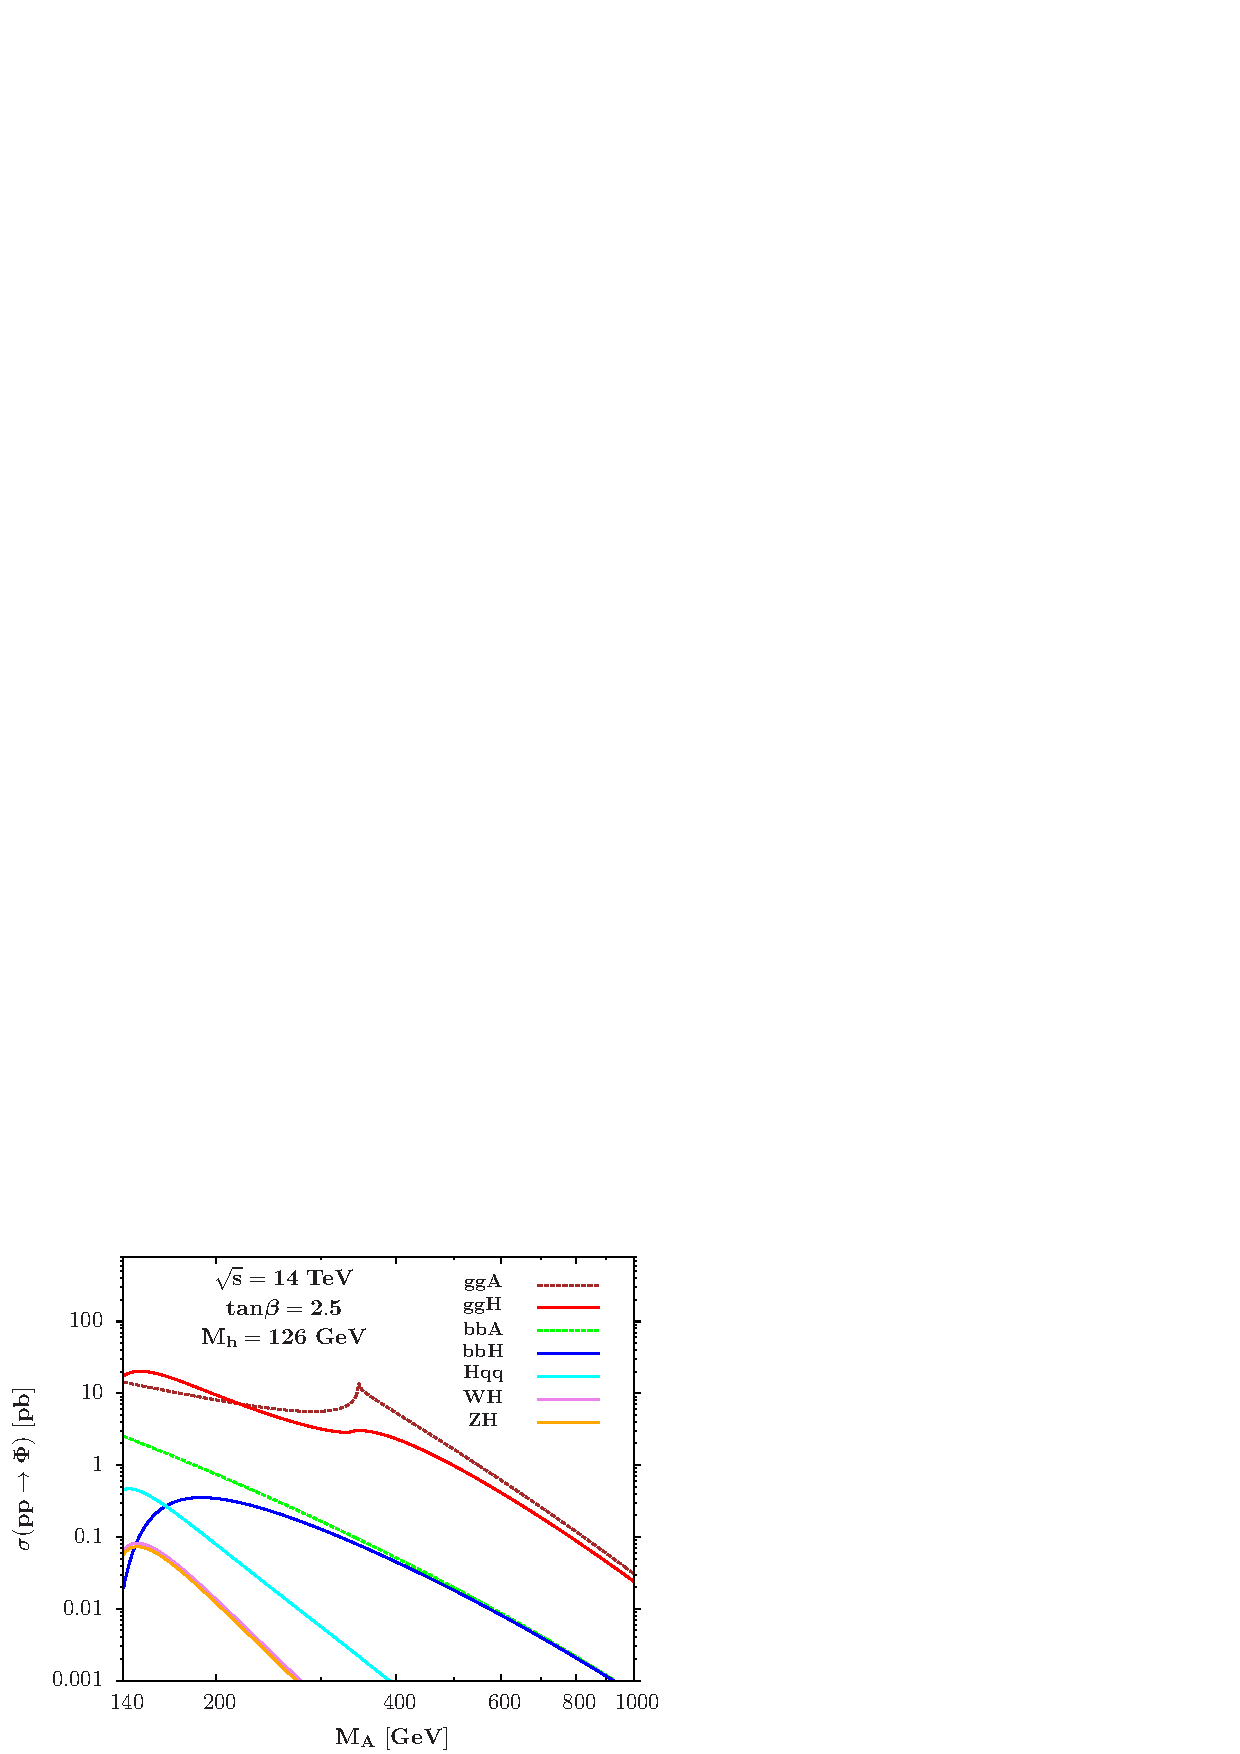
\includegraphics[trim={0cm 0.0cm 9.6cm 21.2cm},clip, scale=0.62]{fig/sm_beyond/Heavy_higgs_prod_xsec.pdf}
& \hspace{-0.3cm} 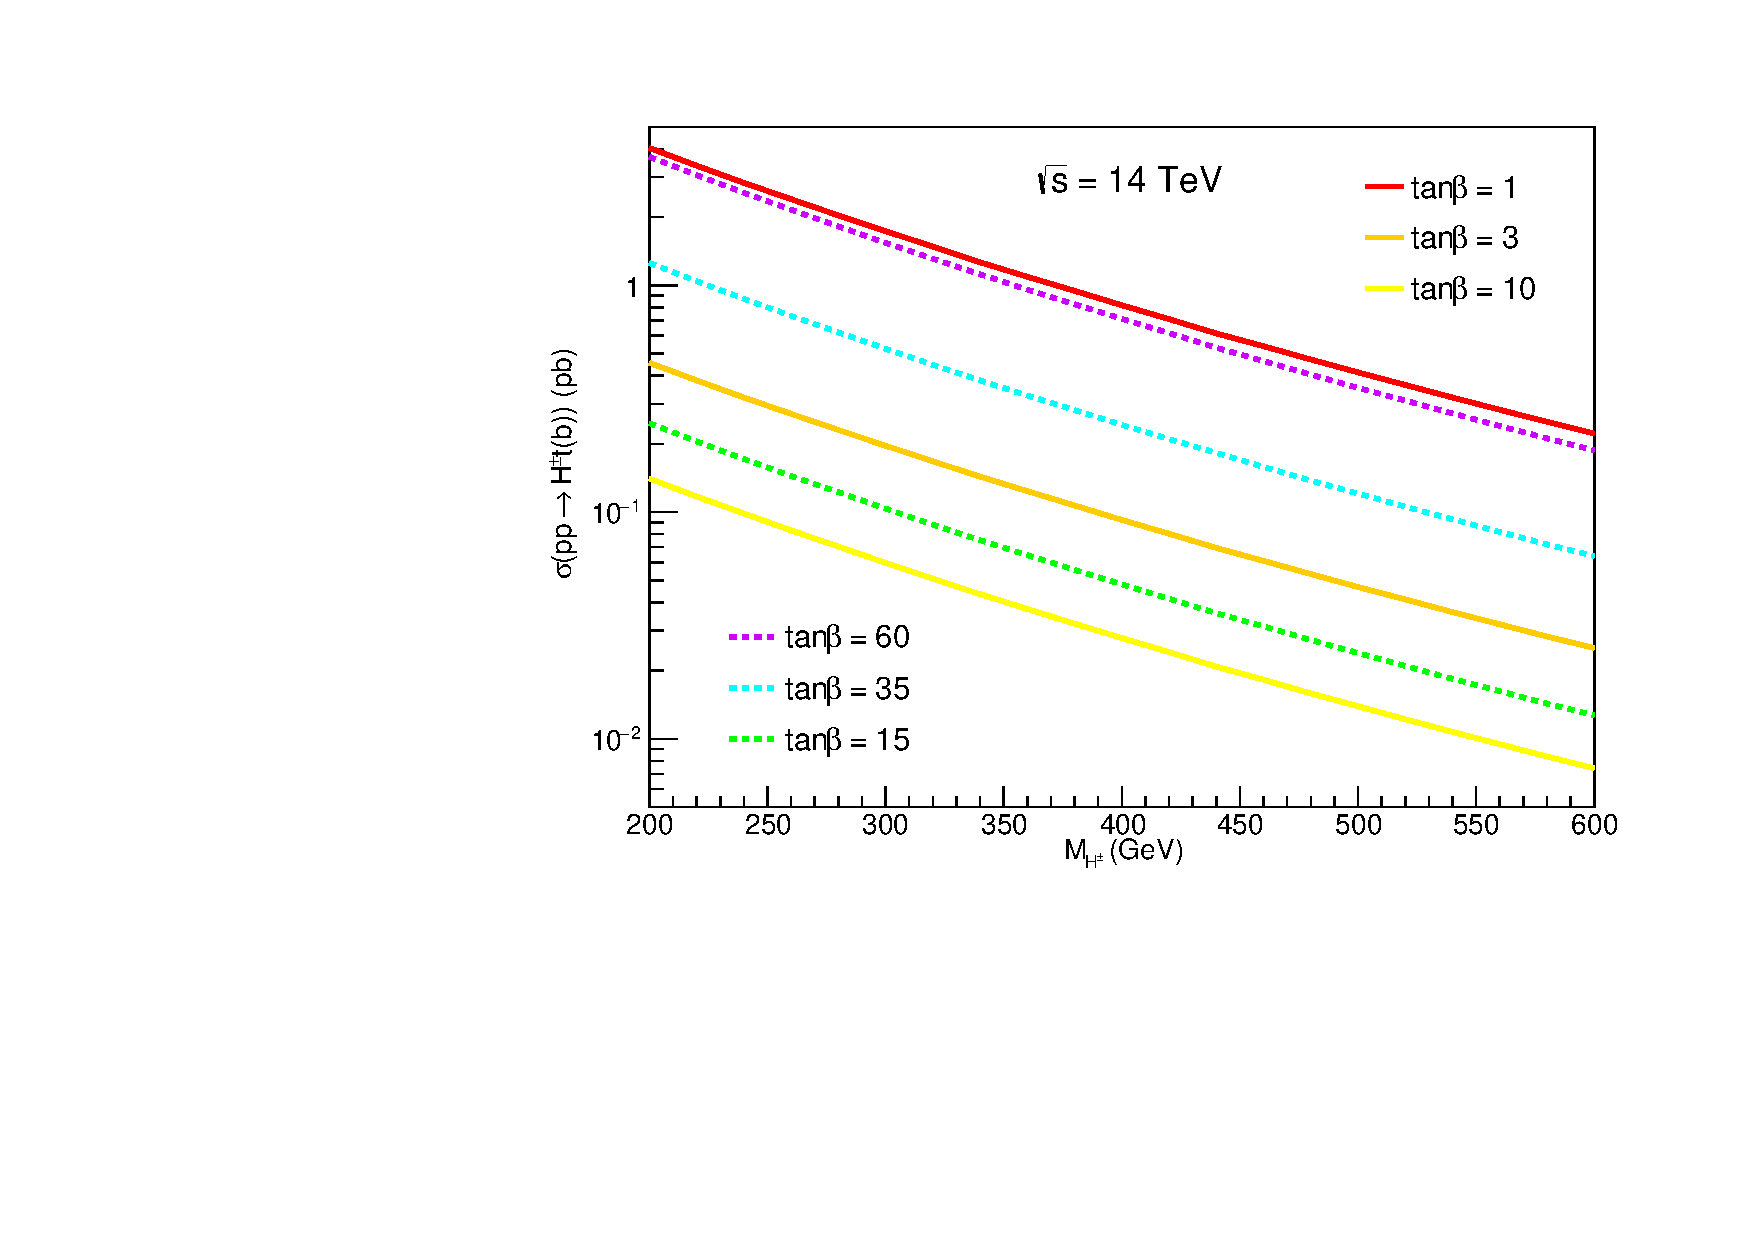
\includegraphics[trim={0cm 0.0cm 0 1cm},clip, scale=0.4]{fig/sm_beyond/plots_xs_Htb_14TeV.pdf}\\
  \qquad\qquad\qquad\qquad ($\mathbf{a}$)\qquad\qquad\qquad&($\mathbf{b}$)\\
\end{tabular}
\caption{(a): Heavy Higgs (neutral) boson production cross sections in MSSM for main channels with $\tan\beta$ = 2.5 and SM Higgs mass is 126\,GeV at $\sqrt{s} = 14\,TeV$ w.r.t M$_{A}$. (b): Charged Higgs production cross sections for a range of $\tan\beta$ values w.r.t to M$_{H^{\pm}}$~\cite{Djouadi:2013vqa,Djouadi:2015jea}. }\label{fig:Heavy_H_prod_xsec}
\end{figure}
\noindent\textbf{Neutral Higgs decay}: The decay of the neutral Higgs ($\Phi$ = H/A) is dictated by the $\tan\beta$ value in a similar pattern as the production because of the coupling sensitivity to $\tan\beta$. In decoupling limits ($\sin\left(\alpha-\beta\right) = 1$), the coupling of the $\mathcal{CP}$-even state is $\frac{\cos\alpha}{\cos\beta}$; as shown in Table~\ref{tab1hmssm:couplings}, it is explicitly equal to $\tan\beta$. For high $\tan\beta \gtrsim 10$, the couplings to b-quark and tau lepton enhanced and it decays exclusively to a $b\bar{b}$ or $\tau^{+}\tau^{-}$ pairs with branching ratios BR($\Phi\rightarrow b\bar{b} \approx 90\%$) and BR($\Phi\rightarrow \tau^{+}\tau^{-} \approx 10\%$) respectively. Decay to $t\bar{t}$ pair is highly suppressed for high $\tan\beta$ range as g$_{\Phi t\bar{t}} \propto 1/\tan\beta$. Other decay modes of $\mathcal{CP}$-even state H like in di-boson ($H\rightarrow VV; V= WW, ZZ$) and decay of $\mathcal{CP}$-odd state into lighter Higgs and Z bosons are strongly suppressed in the alignment limit approximation. For $H\rightarrow hh$ in the limit $M_{H}\gtrsim 2M_{h}$, the coupling $g_{Hhh}$ vanished at high $\tan\beta$~\cite{Baglio:2015wcg}: 
\begin{equation}
g_{Hhh} = 2\sin2\alpha \sin\left(\alpha+\beta\right)-\cos2\alpha\cos\left(\alpha+\beta\right)+3\frac{\Delta M^{2}_{22}}{M^{2}_{Z}}\frac{\sin\alpha}{\sin\beta}\cos\alpha^{2}
\end{equation}
Becomes:
\begin{equation}
\begin{split}
g_{Hhh} \xrightarrow{\text{M}_{A}\gg \text{M}_{z}} -3\Delta \frac{M^{2}_{22}}{M_{Z}^{2}}\times \sin2\beta\\
\sin2\beta \propto \cot\beta \xrightarrow{\tan\beta \gtrsim 10} 0
\end{split} 
\end{equation}  
For $\Phi\rightarrow \gamma\gamma$ channel, the coupling is very small and shows a constant behaviour for $0.3\lesssim \tan\beta \lesssim 10$, which reduces abruptly for $\tan\beta \gtrsim 10$. The same pattern is followed by the $\Phi \rightarrow gg$ channel, but higher coupling compares to $\Phi\rightarrow \gamma\gamma$. For intermediate values of $\tan\beta \approx 5-10$ with M$_{\Phi} < 2m_{t}$, the bosonic decay of $H\rightarrow WW, ZZ$ has a significant contribution as its competition is only with the $H\rightarrow b\bar{b}$ decay. In this limit, the $H\rightarrow t\bar{t}$ decay is suppressed as the phase-space is not feasible. At $\tan\beta$ = 2.5 and $2M_{h} \lesssim M_{\Phi}< 2m_{t}$, $H\rightarrow hh$ and $A\rightarrow hZ$ have prominent branching ratios. Figure~\ref{fig:Heavy_H750_BR} shows branching ratios w.r.t $\tan\beta$ for a specific M$_{\Phi}$ = 750\,GeV. Figure~\ref{fig:Heavy_Hpm_BR}a and b show mass versus branching ratios for $\mathcal{CP}$-odd and $\mathcal{CP}$-even states for $\tan\beta$ = 2.5 and M$_{h}$ = 126\,GeV. 
\begin{figure}[htp]
\centering
%\hspace{-0.3cm} 
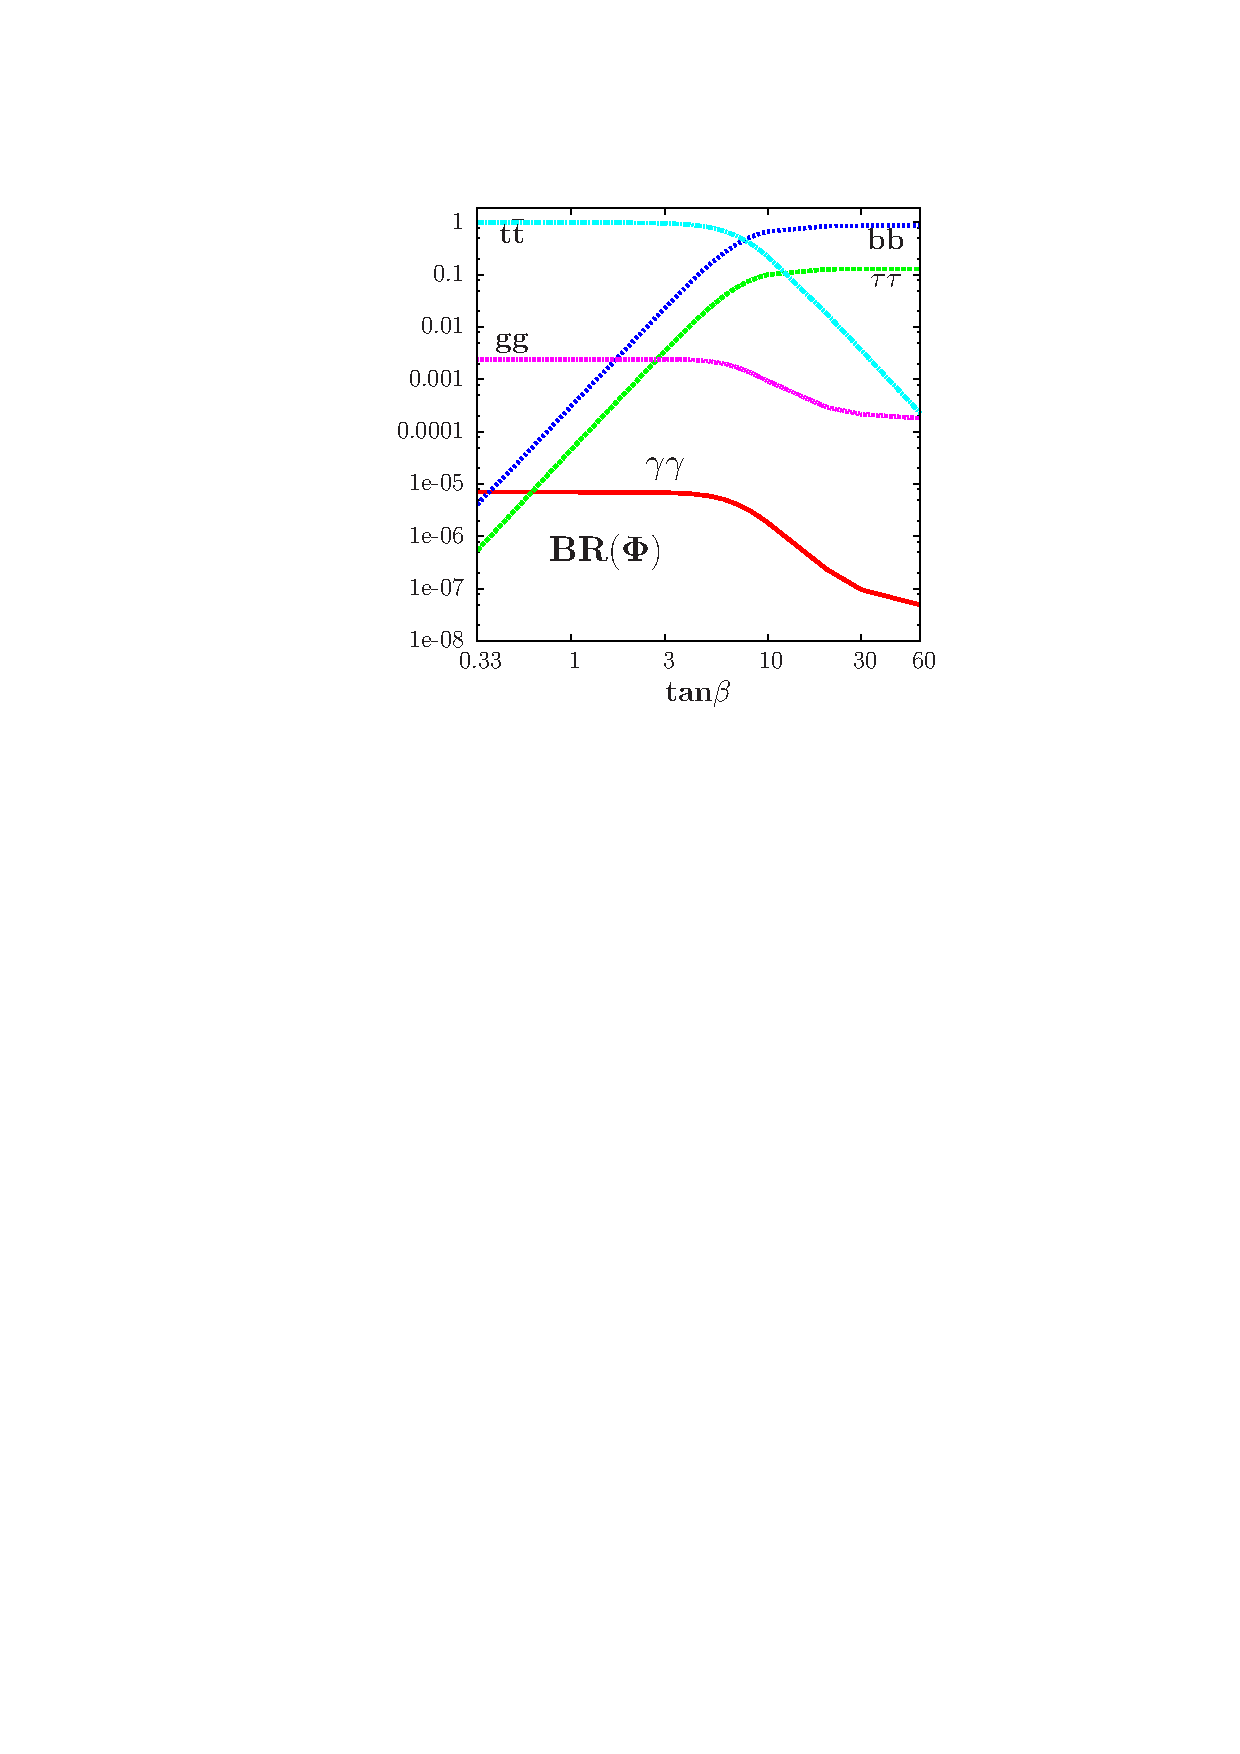
\includegraphics[trim={6.5cm 17.5cm 5.0cm 3.50cm},clip, scale=0.8]{fig/sm_beyond/BR-Atb.pdf}
\caption{The branching ratios of $\Phi$ = H/A in different channels as a function of $\tan\beta$ exploiting the M$_{\Phi}$ = 750\,GeV~\cite{Djouadi:2016eyy}. }\label{fig:Heavy_H750_BR}
\end{figure}

\noindent \textbf{Charged Higgs decay}:
In a high range of $\tan\beta \gtrsim 10$ with M$_{H^{\pm}} \lesssim m_{t} - m_{b}$, the dominant decay of H$^{\pm}$ occurs in the $H^{\pm}\rightarrow \tau\nu$ channel with a small fraction in hadronic decay mode. For high mass range, M$_{H^{\pm}} > m_{t} - m_{b}$, the decay channel M$_{H^{\pm}} \rightarrow tb$ becomes the dominant one while $H^{\pm}\rightarrow \tau\nu$ branching ratio is suppressed. The same pattern for the mentioned mass range is followed for low $\tan\beta$ by these two channels; but this time, the $H^{\pm}\rightarrow \tau\nu$ channel suppressed is more comparable to high $\tan\beta$. For low $\tan\beta$ and M$_{H^{\pm}} \gtrsim 160 $\,GeV, another important channel, $H^{\pm}\rightarrow hW^{\pm}$, comes into play with a smaller branching ratio than the $H^{\pm}\rightarrow tb$ one. Figure~\ref{fig:Heavy_Hpm_BR}c shows the branching ratios as a function of M$_{H^{\pm}}$ for H$^{\pm}$ at $\tan\beta$ = 2.5. Until now, I have discussed all the main decay channels for neutral and charged heavy Higgs in different $\tan\beta$ ranges. However, there are many more that have small contributions. In order to present the complete picture, I have written all of them in the form of total decay width equations. The total decay widths of neutral and charged Higgs are given in expression~\ref{equ:neutral_decay_widths} and~\ref{equ:charged_decay_widths} respectively. For completeness, I mentioned the SUSY decay widths in the formulae. FH is an abbreviation for $\textsc{FEYNHIGGS}$ and HD stands for $\textsc{HDECAY}$ programs commonly used for decay widths and branching-ratio calculation of the Higgs boson. More detail can be found here~\cite{Dittmaier:2012vm}.
\begin{equation}\label{equ:neutral_decay_widths}
\begin{split}
\Gamma_{\Phi} = \Gamma^{\text{FH}}_{\Phi \rightarrow\tau^{+}\tau^{-}} + \Gamma^{\text{FH}}_{\Phi \rightarrow\mu^{+}\mu^{-}} + \Gamma^{\text{FH/P4f}}_{\Phi \rightarrow \text{W}^{*}\text{W}^{*}} + \Gamma^{\text{FH/P4f}}_{\Phi \rightarrow \text{Z}^{*}\text{Z}^{*}}\\
+ \Gamma^{\text{HD}}_{\Phi \rightarrow b\bar{b}} + \Gamma^{\text{HD}}_{\Phi \rightarrow t\bar{t}} + \Gamma^{\text{HD}}_{\Phi \rightarrow c\bar{c}} + \Gamma^{\text{HD}}_{\Phi \rightarrow gg} + \Gamma^{\text{HD}}_{\Phi \rightarrow \gamma \gamma} + \Gamma^{\text{HD}}_{\Phi \rightarrow \text{Z} \gamma}\\
+ \Gamma^{\text{FH}}_{\Phi \rightarrow \text{Zh}} + \Gamma^{\text{FH}}_{\Phi \rightarrow \text{hh}} + \Gamma^{\text{FH}}_{\Phi \rightarrow \text{ZA}} + \Gamma^{\text{FH}}_{\Phi \rightarrow \text{AA}}  + \Gamma^{\text{HD}}_{\Phi \rightarrow \text{H}^{\pm}\text{W}^{\mp}} + \Gamma^{\text{FH}}_{\Phi \rightarrow \text{SUSY}}
\end{split}
\end{equation}
\begin{equation}\label{equ:charged_decay_widths}
\begin{split}
\Gamma_{\text{H}^{\pm}} = \Gamma^{\text{FH}}_{\text{H}^{\pm} \rightarrow\tau\nu_{\tau}} + \Gamma^{\text{FH}}_{\text{H}^{\pm} \rightarrow\mu\nu_{\mu}} + \Gamma^{\text{FH}}_{\text{H}^{\pm} \rightarrow \text{hW}} + \Gamma^{\text{FH}}_{\text{H}^{\pm} \rightarrow \text{HW}} + \Gamma^{\text{FH}}_{\text{H}^{\pm} \rightarrow \text{AW}}\\
+ \Gamma^{\text{HD}}_{\text{H}^{\pm} \rightarrow \text{tb}} + \Gamma^{\text{HD}}_{\text{H}^{\pm} \rightarrow \text{ts}} + \Gamma^{\text{HD}}_{\text{H}^{\pm} \rightarrow \text{td}} +  \Gamma^{\text{HD}}_{\text{H}^{\pm} \rightarrow \text{cb}} + \Gamma^{\text{HD}}_{\text{H}^{\pm} \rightarrow \text{cs}} + \Gamma^{\text{HD}}_{\text{H}^{\pm} \rightarrow \text{cd}}\\
+ \Gamma^{\text{HD}}_{\text{H}^{\pm} \rightarrow \text{ub}} + \Gamma^{\text{HD}}_{\text{H}^{\pm} \rightarrow \text{us}} + \Gamma^{\text{HD}}_{\text{H}^{\pm} \rightarrow \text{ud}} + \Gamma^{\text{HD}}_{\text{H}^{\pm} \rightarrow \text{SUSY}}
\end{split}
\end{equation}
\begin{figure}[htp]
\centering
\begin{tabular}{ccc}
\hspace{-0.2cm}
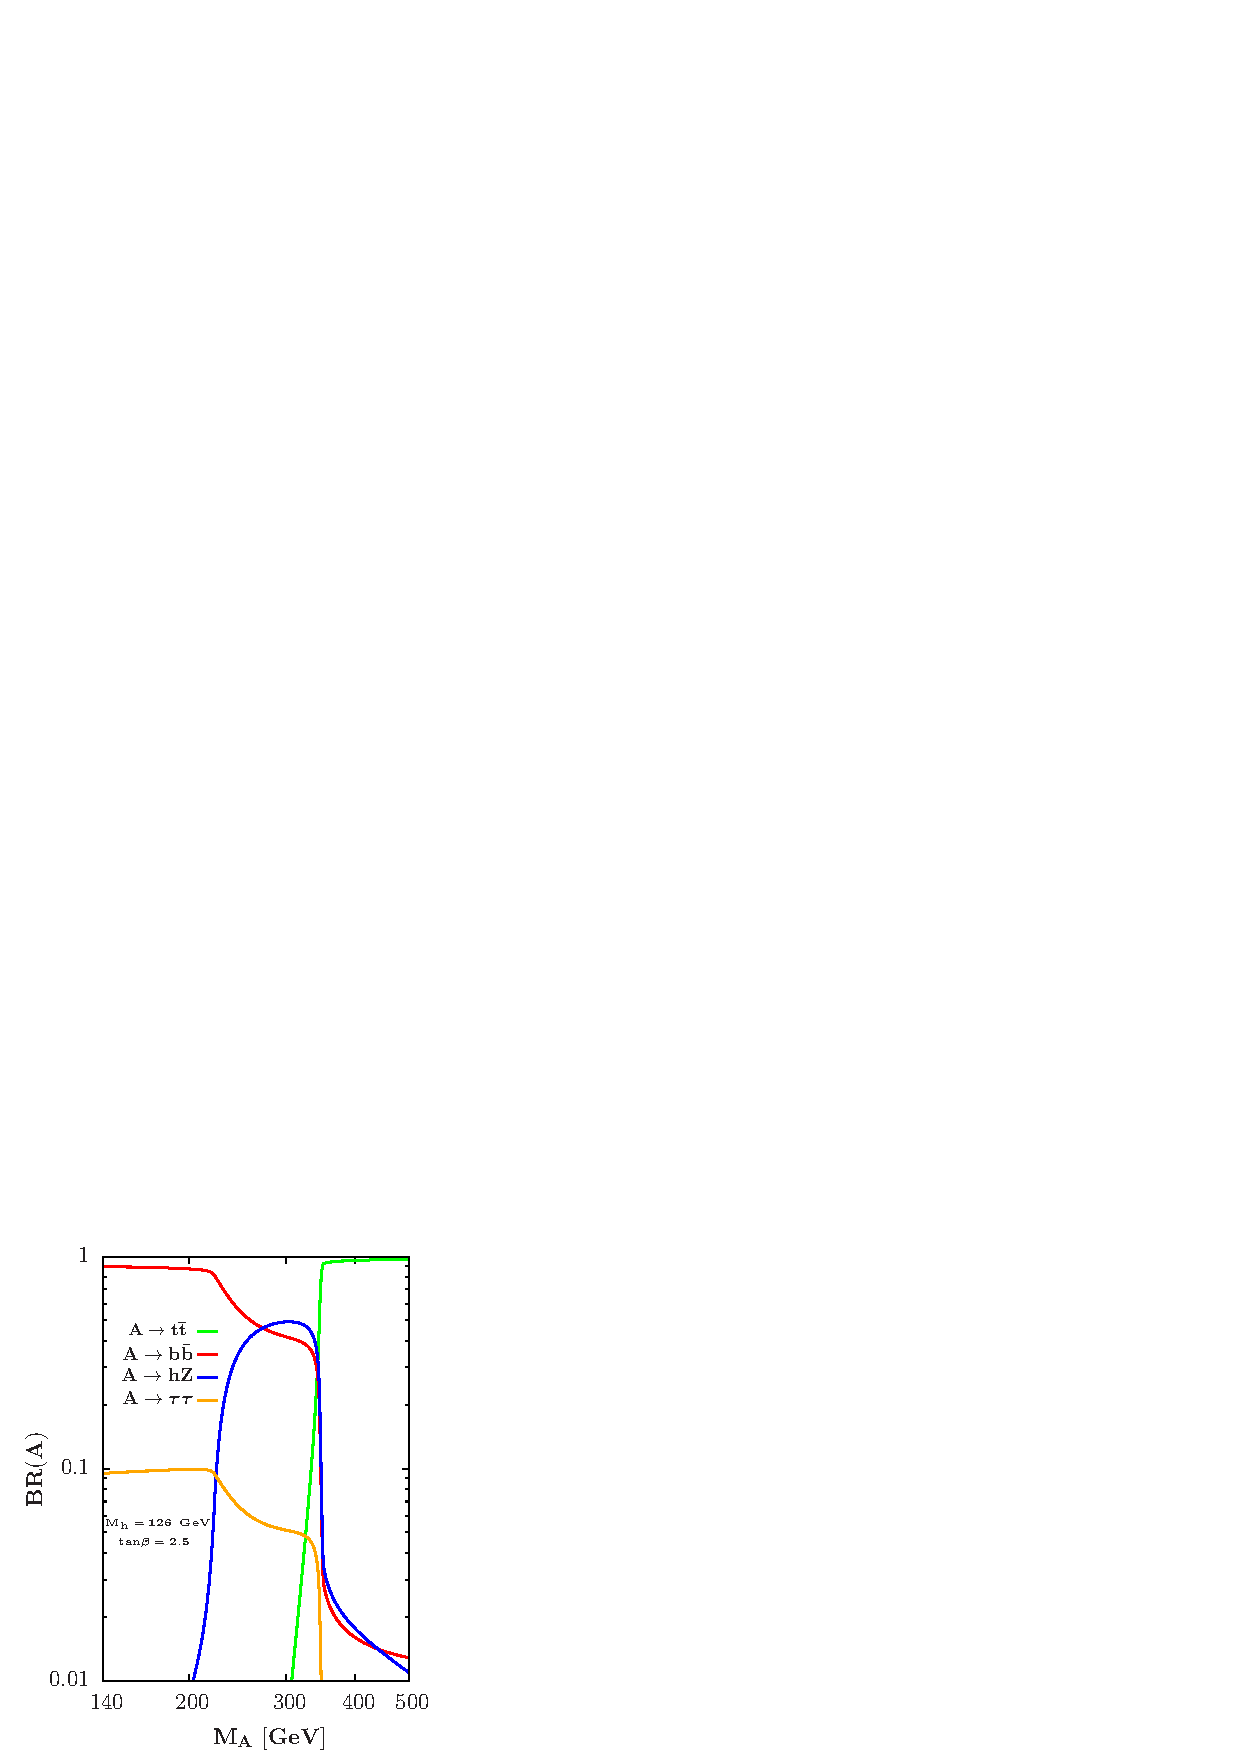
\includegraphics[trim={0cm 0cm 13cm 21cm},clip, scale=0.58]{fig/sm_beyond/A_br.pdf}
& \hspace{-0.65cm} 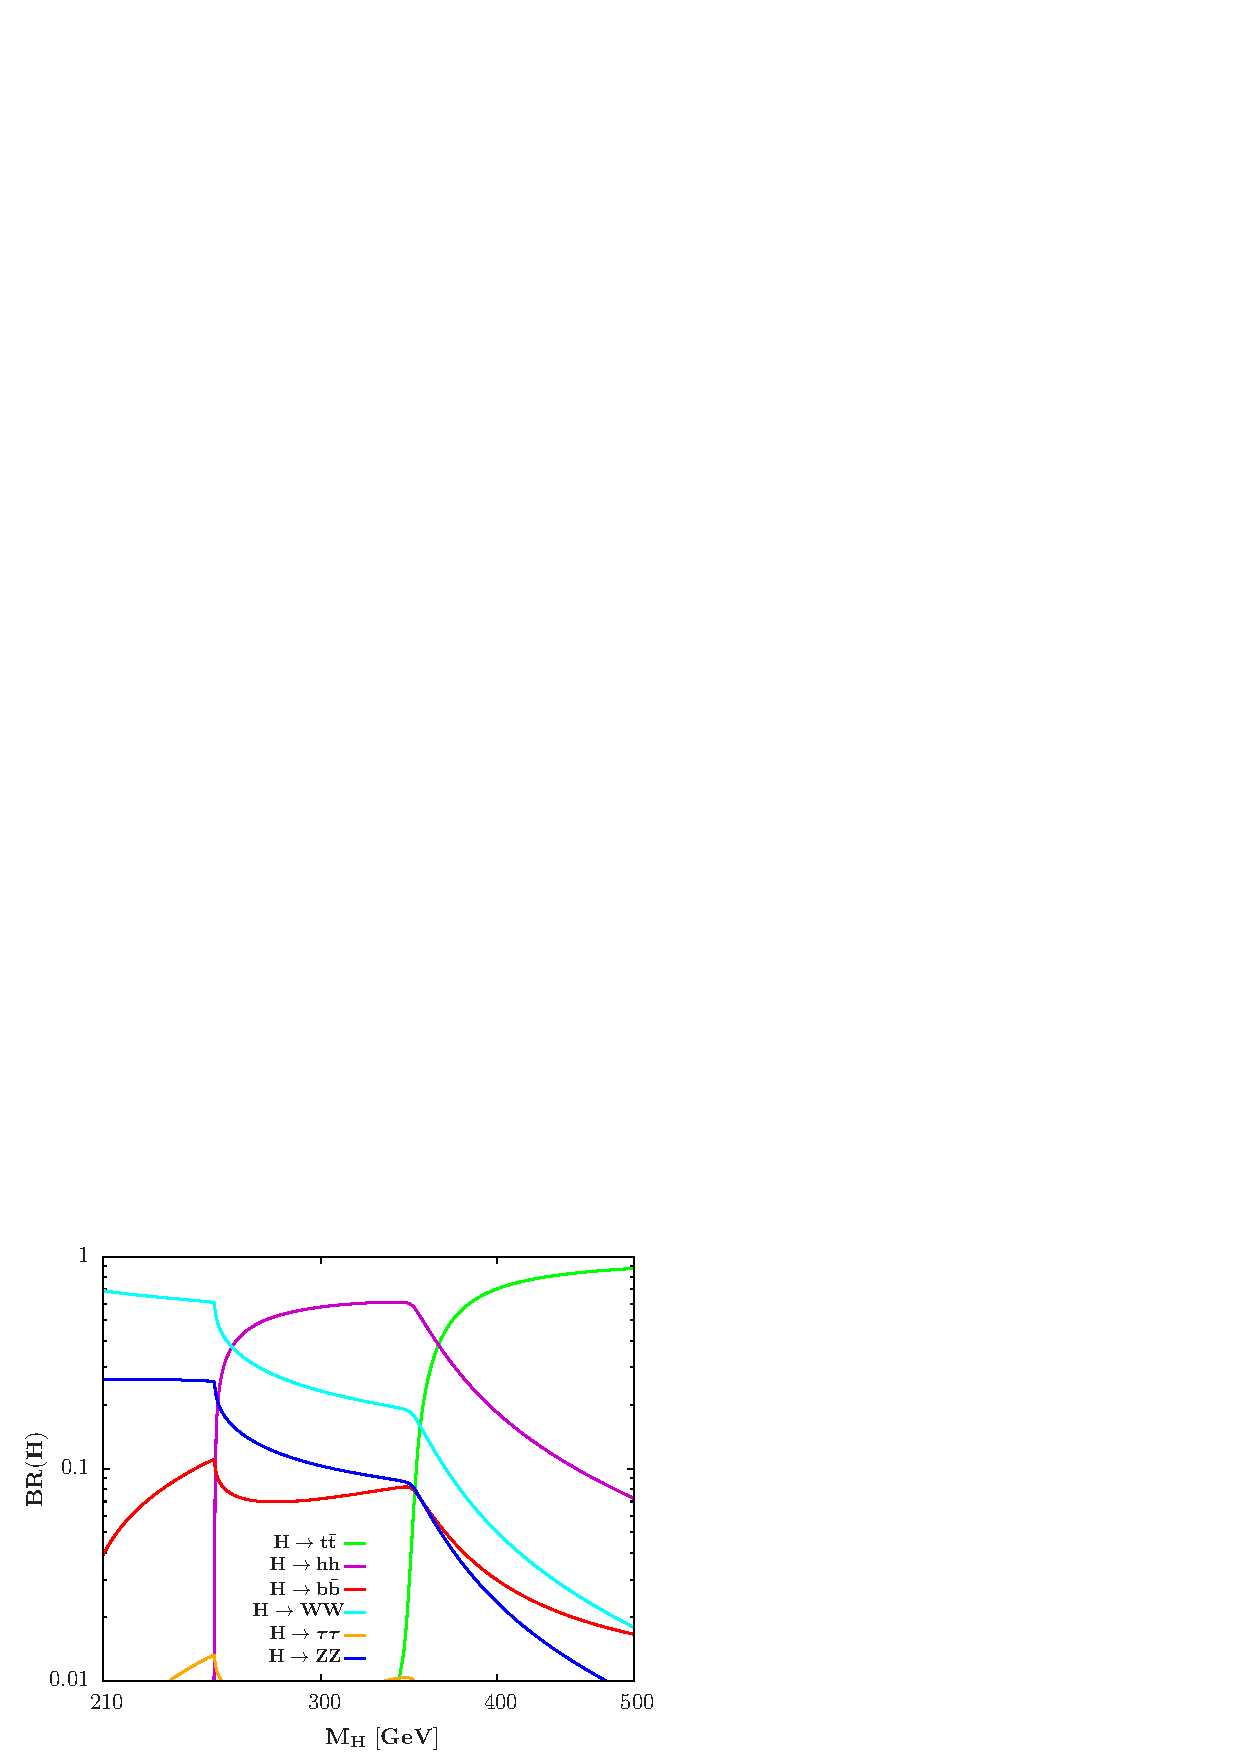
\includegraphics[trim={0.0cm 0cm 9.5cm 21cm},clip, scale=0.58]{fig/sm_beyond/H_br.pdf}
& \hspace{-0.65cm} 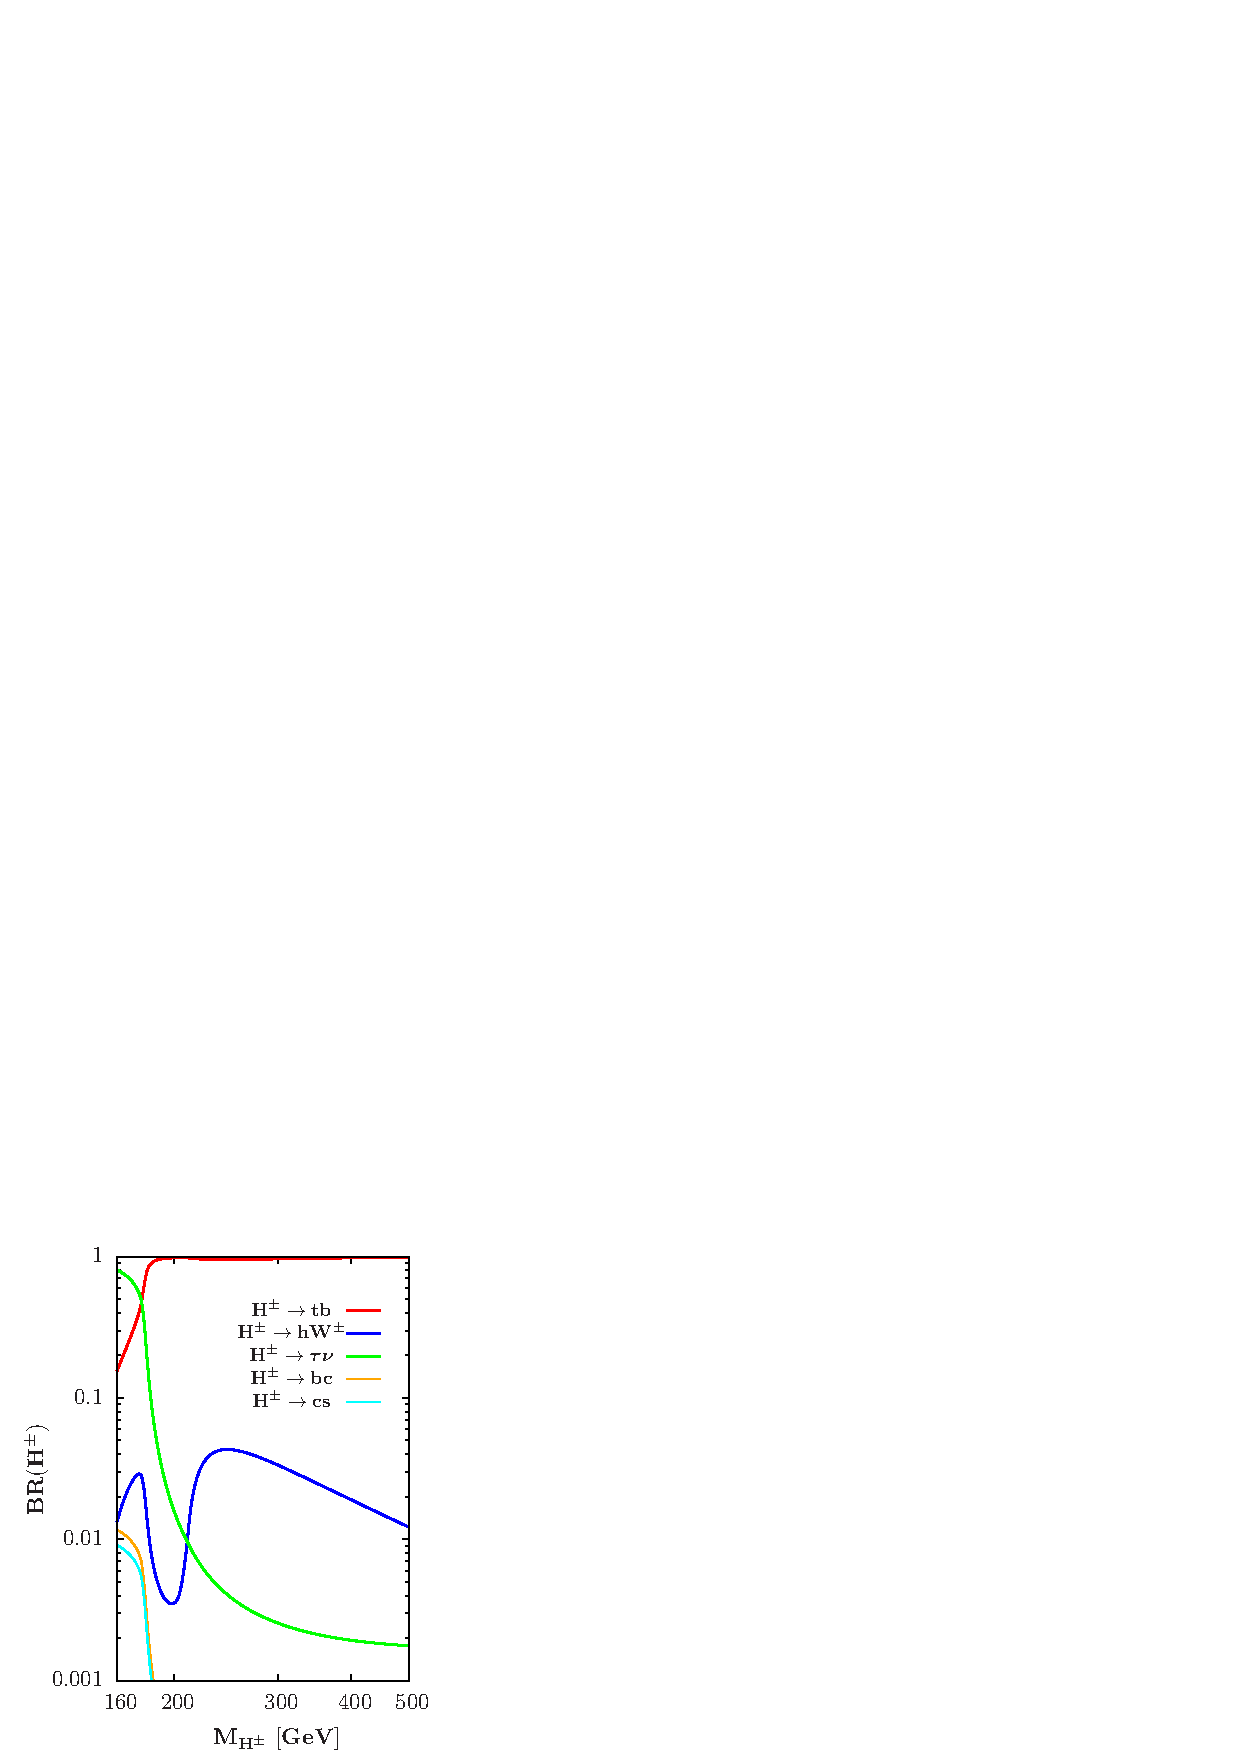
\includegraphics[trim={0.0cm 0cm 13cm 21cm},clip, scale=0.58]{fig/sm_beyond/H_pm_br.pdf}\\
  \qquad ($\mathbf{a}$)\qquad\qquad&($\mathbf{b}$)\qquad\qquad&($\mathbf{c}$)\\
\end{tabular}
\caption{Heavy Higgs decay branching ratios in MSSM, (a) pseudo scalar Higgs A, (b) Scalar Higgs H and (c) charged Higgs (H$^{\pm}$) with $\tan\beta$ = 2.5 and SM Higgs mass is 126~\cite{Djouadi:2013vqa}. }\label{fig:Heavy_Hpm_BR}
\end{figure}
\noindent \subsection{The $\Phi \rightarrow t\bar{t}$ channel with interference from the SM $gg \rightarrow t\bar{t}$}
\textbf{Introduction to interference:} In particle physics, a process is represented by one or more Feynman diagrams and the resultant amplitude is expressed in terms of the matrix element. For a given process, interference is the contribution of the cross terms of different processes to the final amplitude that introduces a peak, dip, nothingness, or a more complex peak-dip or dip-peak structure. It can be considered to be a similar phenomenon as quantum wave interference. Interference depends on the physics model and affects different kinematics of the searched particle in different ways. Most particle discoveries are carried out by simply confirming a resonant peak in the invariant or transverse mass distribution above the continuum backgrounds, like $J/\Psi$ meson, $W/Z$ bosons, Higgs ($h$) boson, and top quark. Currently, most new LHC physics searches focus on the same search strategy by examining the access above the continuum background. But in some cases, the kinematics (mass, $p_{T}$) of the searching particle are not pure Breit-Wigner (BW) resonance peak but instead, a modified shape from the interfering background or other resonance. The complicated dip-peak or peak-dip structure is more sensitive to new physics than the simple resonant peak. This was first realised in the $gg\rightarrow\Phi\rightarrow t\bar{t}$ channel~\cite{Gaemers:1984}. This channel, along with interference effect, is studied in this thesis and will be explained in detail after the general introduction to the interference is given. 

Consider a two-body scattering $ab\rightarrow {cd}$ whose partonic differential cross section w.r.t angular variable $z\cos\theta^{*}$, where $\theta^{*}$ is the scattering angle in the centre-of-mass frame, can be expressed as~\cite{Jung:2015gta}:   
\begin{equation}\label{equ:gen_interference}
\frac{d\hat{\sigma}}{dz}=\frac{1}{32\pi\hat{s}}\sum \left| \mathcal{A}_{\text{bg}}e^{i\phi_{\text{bg}}}+\frac{M^{2}}{\hat{s}-M^{2}+iM\Gamma}.\mathcal{A}_{\text{res}}e^{i\phi_{\text{res}}} \right|^{2}.
\end{equation}
In Eq.~\ref{equ:gen_interference}, the sum pertains to all spin and colour components; $\hat{s}$ is the partonic energy and $\phi_{bg,res}$ is the complex phase of background and resonant part respectively. $\mathcal{A}_{bg}$ shows the continuum background amplitude and the term $\mathcal{A}_{res}$ is the resonance amplitude for the searching particle with mass M and width $\Gamma$. Expanding the square and re-arranging, we get Eq.~\ref{equ:split_inter} where we define new terms, $\sigma_{int}$, R, $\omega$ and $\phi = \phi_{res}-\phi_{bg}$ with definitions in Eq.~\ref{equ:inter_variables}.  

\begin{equation}\label{equ:split_inter}
\hat{\sigma}=\hat{\sigma}_{\text{bg}}+\frac{M^{4}}{\left(\hat{s}-M^{2}\right)^{2}+M^{4}\omega^{2}}\times\left[\frac{2\left(\hat{s}-M^{2}\right)}{M^{2}}\hat{\sigma}_{\text{int}}c_{\phi}+\hat{\sigma}_{\text{res}}\left(1+\frac{2\omega}{R}s_{\phi} \right) \right]
\end{equation}
where c$_{\phi}$ = cosine$\phi$ and s$_{\phi}$ = sine$\phi$.
\begin{equation}\label{equ:inter_variables}
\begin{split}
\hat{\sigma}_{\text{bg,res}}=\frac{1}{32\pi\hat{s}}\int dz \sum \mathcal{A}^{2}_{\text{bg,res}},\\
\hat{\sigma}_{\text{int}}e^{i\phi}=\frac{1}{32\pi\hat{s}}\int dz \sum \mathcal{A}_{\text{bg}}\mathcal{A}_{\text{res}}e^{i\left(\phi_{\text{res}}-\phi_{\text{bg}}\right)},\\
R=\frac{\hat{\sigma}_{\text{res}}}{\hat{\sigma}_{\text{int}}},\qquad \omega \equiv \frac{\Gamma}{M}.
\end{split}
\end{equation}

$\omega$, R and  $\phi$ are parameters of interest, with the latter two being relative strength and phase difference between signal resonance and background continuum respectively. The second interference term in equation~\ref{equ:split_inter} further consists of two parts – the real with $\text{c}_{\phi}$ and imaginary s$_{\phi}$, which decides the final interference pattern. The well-known peak-dip or dip-peak structure arises from the real interference part with s$_{\phi}$ = 0 with a final shift in the resonance peak position. We focus on the pure resonance as well as the peak-dip structure of the signal in this analysis. The imaginary term also makes the shape interesting at specific conditions of $\phi$ and factor C, where C is defined as:
\begin{equation}\label{equ:correction_term}
C \equiv \left(1+\frac{2\omega}{R}s_{\phi} \right).
\end{equation} 
At $\phi=-\pi /2$ and C < 0, the $gg\rightarrow\Phi\rightarrow AB$ line adopted a pure dip shape, as shown in Fig.~\ref{fig:dip_peak_nothing_H_A} by the green line. On the contrary, the access can be achieved by C > 0 shown by the orange line in Fig.~\ref{fig:dip_peak_nothing_H_A}, where its amplitude can be increased or decreased relative to pure resonance (dashed-orange line) by varying the value of $\phi$. At $\phi=-\pi /2$ and C = 0, the line shape becomes more interesting when both the real and imaginary part disappear and the signal line now runs parallel to the continuum background. These types of shapes are termed as ``nothingness'' and need more careful treatment. The interference pattern arising from the purely imaginary part is even around the resonance mass, Fig.~\ref{fig:dip_peak_nothing_H_A} green and orange line. This type of interference significantly changes the total signal rate and doesn't depend on the precise magnitude of the resonance width. All the above defined signal structures demand a new search strategy as compared to the simple resonance we seek. 

\begin{figure}[htp]
\centering
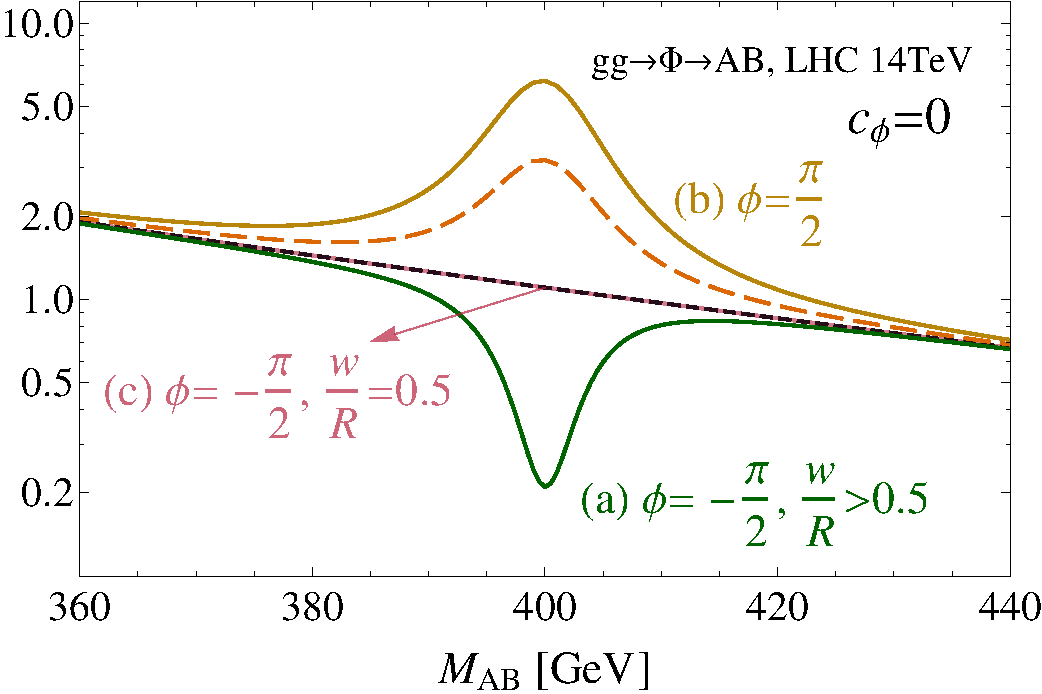
\includegraphics[scale=0.5]{fig/sm_beyond/dip_peak_nothing.pdf}
\caption{Resonance shapes after pure imaginary interference (c$_{\phi}$ = 0) with mass = 400\,GeV, $\Gamma$ = 10\,GeV and R = 0.035. Green line is pure dip, orange is access, orange-dashed is pure resonance, red is nothingness and solid black is continuum background. Arbirary units are used on y-axis~\cite{Jung:2015gta}. }\label{fig:dip_peak_nothing_H_A}
\end{figure}
%------------------------------------------------------------------

The dip-peak or peak-dip structure around the resonance mass is the most common signal shape studied in the literature. This is the standard case that doesn't affect the total rate and instead only changes the signal line shape. It arises from the real part of the interference term, c$_{\phi}$ in equation~\ref{equ:split_inter} when $\phi$ = 0 or $\pi$. From Eq.~\ref{equ:split_inter}, it is evident that the real part (c$_{\phi}$) is odd around the resonance mass compared to the imaginary part (s$_{\phi}$), which is even. That's why the real interference term doesn't alter the signal rate and instead provides an arc-type profile around $\sqrt{\hat{s}}$ values close to the scalar mass. The schematic signal line shape corresponding to the real interference part is shown in Fig.~\ref{fig:schematic_lineshape} by an orange dashed line as a function of the centre-of-mass energy, $\sqrt{\hat{s}}$.  
\begin{figure}[htp]
\centering
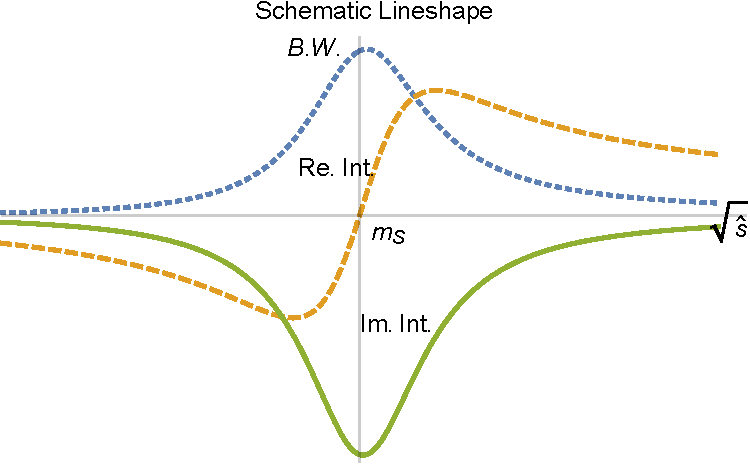
\includegraphics[trim={0cm 0.0cm 0 0.5cm},clip, scale=0.7]{fig/sm_beyond/schematic_lineshape.pdf}\\
\caption{The blue dotted line is the signal component, namely the Breit-Wigners resonance; the orange dashed line is the interference between signal and continuum background produced by the real component of the propagator; and the solid green line is the interference proportional to the imaginary part of the propagator as a function of the centre-of-mass energy, $\sqrt{\hat{s}}$~\cite{Carena:2016npr}. }\label{fig:schematic_lineshape}
\end{figure}
%------------------------------------------------------------------

Now specifically consider the analysis included in this thesis related to the search for heavy Higgs in the $t\bar t$ final state, $gg\rightarrow A/H \rightarrow t\bar t$, the heavy Higgs boson ($\phi_{i}$ = A/H) is the additional s-channel contribution shown in leading order diagrams~\ref{fig:ggh_production_to_ttbar}. 
\begin{figure}[htp]
\centering
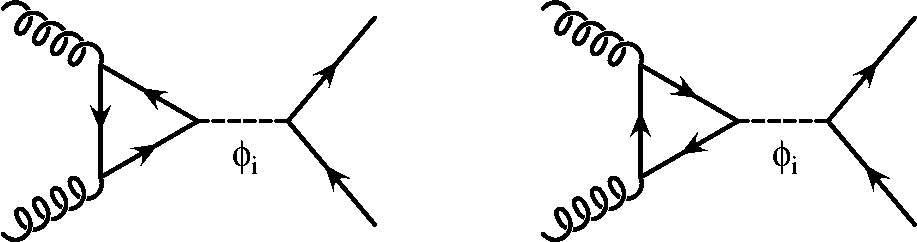
\includegraphics[scale=0.7]{fig/sm_beyond/gg-higgs-tt.pdf}\\
\caption{Tree-level Feynman diagrams for the heavy Higgs ($\phi_{i}$ = A/H) production via gluon-gluon fusion and decay into fermion (top quarks) pair. The only differenc between the two diagrams is the clock and anti-clock wise fermionic loop~\cite{Bernreuther:2015fts}. }\label{fig:ggh_production_to_ttbar}
\end{figure}
Although all quarks can contribute to the fermionic loop, in low $\tan\beta$ region, the bottom quark loop is strongly suppressed and the top quark is the dominant candidate in the loop. Other lighter quarks have less contributions than the b-quark and can safely be neglected. With higher mass than the $t\bar t$ threshold, M$_{A/H}\geq 2m_{t}$, and low $\tan\beta$, heavy Higgs decays exclusively into a top quark pair. The SM background $gg\rightarrow t\bar t$ diagrams are shown in Fig.~\ref{fig:ttbar_prod}, produced by hadron colliders at high energy, interfere with the signal. The signal amplitude for $\mathcal{CP}$-even and odd state can be written in terms of fermionic loop (top quark loop) function:
\begin{equation}\label{equ:A_H_amplitudes}
\mathcal{A}^{\mathcal{CP}-even} = y_{t}^{2}A^{H}_{\frac{1}{2}}(\tau_{t}), 
\mathcal{A}^{\mathcal{CP}-odd} = \tilde{y}_{t}^{2}A^{A}_{\frac{1}{2}}(\tau_{t})
\end{equation}
Where $A^{H/A}_{\frac{1}{2}}(\tau_{t})$ is the loop function given by Eq.~\ref{equ:form_factors}; the constants in the equation have been omitted for simplicity. I want to discuss the behaviour of the $\mathcal{CP}$-even and odd states based on the fermonic (top quark in our case) loop functions here, as they are the only source of additional phase $\phi$. In Fig.~\ref{fig:loop_function_phase}a, the phase of the loop function is drawn as a function of the of $\sqrt{\tau}\equiv \sqrt{\hat{s}}/2m_{t}$ – the solid red line for scalar and blue-dashed line for pseudo-scalar particle. On the upper horizontal axis, centre-of-mass energy is drawn in GeV units for the top quark in the loop. At lower values of $\tau \ll$ 1, the phase of both states is nearly constant, but just after crossing the threshold of on-shell top pair, $\sqrt{\hat{s}} \approx 2m_{t}$, at $\tau\approx 1$ the phase changes quickly and at larger $\tau$ the variation become slow. The fact is that at $\tau\geq 1$, the imaginary part of the loop function rises quickly and then decreases slowly for increasing values of $\tau$. It is clear that the phase of $\mathcal{CP}$-odd always reaches faster as compared to $\mathcal{CP}$-even. In Fig.~\ref{fig:loop_function_phase}b, the phase is drawn as a function of the mass M$_{A/H}$ for the two states, $\mathcal{CP}$-even (H) blue band and $\mathcal{CP}$-odd (A) red band. Different tan$\beta$ (vacuum expectation values for two states) values, 2, 5 and 10 are represented by solid, dashed, and dotted lines respectively. The upper-horizontal axis is labelled with $\tau$ values. It shows that $\mathcal{CP}$-odd state attains higher phase before the $\mathcal{CP}$-even for the whole mass range. At typical value of tan$\beta$ = 2, $\mathcal{CP}$-odd reaches to $-\pi$/2 at M$_{A}$ = 850\,GeV while $\mathcal{CP}$-even at M$_{H}$ = 1170\,GeV.    
\begin{figure}[htp]
\centering
\begin{tabular}{cc}
\hspace{-0.3cm}
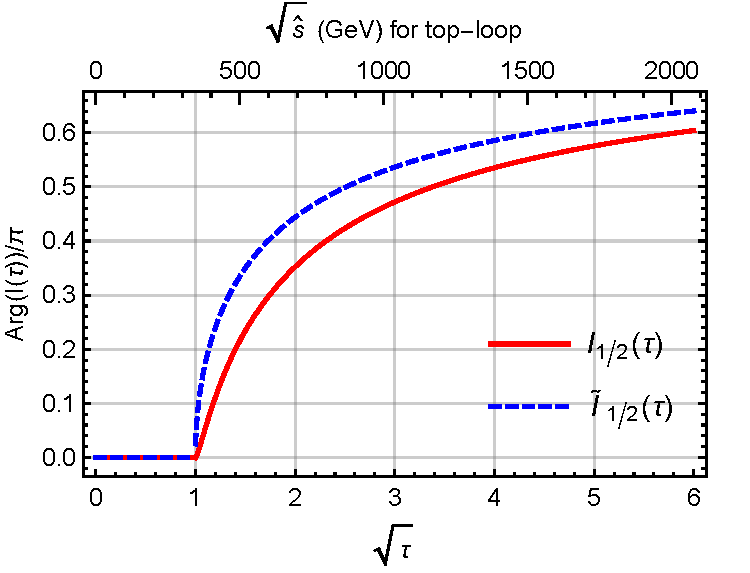
\includegraphics[scale=0.6]{fig/sm_beyond/loop_function_phase.pdf}
& \hspace{-0.4cm} 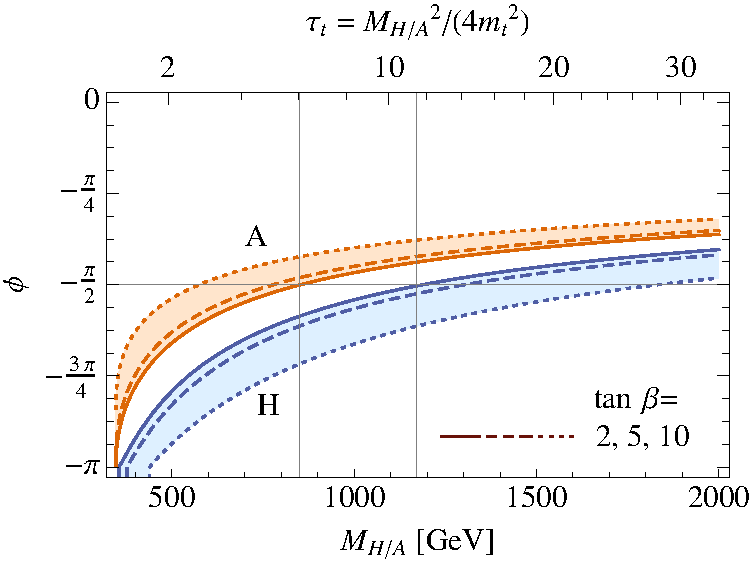
\includegraphics[scale=0.603]{fig/sm_beyond/fig_phase_A_H.pdf}\\
  \qquad ($\mathbf{a}$)\qquad\qquad&($\mathbf{b}$) \\
\end{tabular}
\caption{(a) The phase of the loop functions in units of $\pi$ as a function of $\tau$ for scalar (red line) and pseudoscalar (blue-dashed line) respectively. The upper-horizontal axis is labelled with the corresponding centre-of-mass energy $\sqrt{\hat{s}}$ in units of GeV for the case of a top quark loop~\cite{Carena:2016npr}. (b) shows the relative phase $\phi$ between continuum $gg\rightarrow t\bar{t}$ and resonace $gg\rightarrow \Phi \rightarrow t\bar{t}$ w.r.t M$_{H/A}$ at different $tan\beta$ values (2, 5, 10) with $\tau_{t} = M^{2}_{H/A}/(4m_{t}^{2})$ at the upper-horizontal axis. For all values of $tan\beta$, the $-\pi/2$ condition achieved by $\mathcal{CP}-$odd state ($A$) much faster than the $\mathcal{CP}-$even state ($H$) shown by vertical lines~\cite{Jung:2015gta}. }\label{fig:loop_function_phase}
\end{figure}
%------------------------------------------------------------------

Until now, we studied the $\mathcal{CP}$-conserving scenario, where the $\mathcal{CP}$-even and odd state don't interfere and the resultant cross section is the sum of the two independent states. In case of nearly degenerate heavy Higgs states ($A, H, H^{\pm}$), as predicted by MSSM, the two $\mathcal{CP}$ states interfere with each other. This interference is small in comparison to the SM $t\bar t$ background interference but still allows for a rich phenomenology in this channel. Interference between the two $\mathcal{CP}$ states depends on the masses, separation between the masses, widths, and the phase of the two scalars. The new interference produces another minor peak-dip between the two masses, which needs special consideration~\cite{Carena:2016npr}. We considered only the top quark in the loop and neglected light quarks because of their small contributions. If we consider some moderate value of $\tan\beta$, the bottom quark loop contribution scales as $\tan\beta$, while the top quark scales $1/\tan\beta$. The bottom and top quarks loops can also interfere constructively or destructively, depending upon the relative phase between them. Although the bottom-quark contribution only provides a small correction, it makes the study more interesting. Many BSM theories like composite Higgs models~\cite{vonGersdorff:2015fta} and flavour models motivated the idea of vector-like quarks. These vector-like quarks contribute to the loop and change the phenomenology of this channel. SUSY predicts the scalar partners of the SM fermions which may also contribute to the gluon-gluon-scalar effective coupling. But for higher masses, like heavy stop, the current data is not sufficient to further probe and impose some relevant constraints.      
%---------------------------------------------------------------------------

\noindent \textbf{The two observables, mass of $t\bar t$ and Collins Soper angle:}
The search for heavy Higgs boson in the $t\bar t$ final state exploits two variables – the mass of $t\bar t$ and angular variable $\cos\theta^{*}$ – for the final statistical evaluation. The top quark production and decay in different channels are discussed in Sec.~\ref{subsec:top_quark} and the $t\bar t$ system reconstruction will be explain in detail in section~\ref{subsec:ttbar_reco}. The angular variable, commonly known as Collins-Soper angle~\cite{collins_soper}, is sensitive to the spin of the intermediate heavy Higgs boson decaying into $t\bar t$ and very less affected by the initial state radiation. Consider the collision of two non-collinear hadrons with momenta $p_{1}$ and $p_{2}$ in the rest mass frame of the $t\bar t$. The resultant top and anti-top quark will not be back-to-back and will have non-zero transverse momentum. The Collins-Soper angle $\theta$ is defined as being the angle between the axis that bisects the angle between $p_{1}$ and $p_{2}$ and the top quark momentum in the $t\bar t$ rest frame.

In the SM process, $gg\rightarrow t\bar t$, the squared amplitude is proportional to the cosine of $\theta$ which is shown by a complicated relation~\ref{equ:collins-soper-sm}:
\begin{equation}\begin{split}
{\left|\mathcal{M}\left(gg\rightarrow t\bar t \right)\right|}^{2} \sim \\
\frac{s\left(7 + 9\cos^{2}\theta \right) - 36m_{t}^{2}\cos^{2}\theta}{\left( sc_{-} + 4m_{t}^{2}\cos^{2}\theta \right)^{2}}\\
\left[ s^{2}c_{+}c_{-} + 2sm_{t}^{2}\left(3c_{-}^{2} + c_{+}^{2} \right) -4m_{t}^{2} \left(3c_{-}^{2}+c_{+}^{2}+c_{-} \right)\right],
\label{equ:collins-soper-sm}
\end{split}
\end{equation} 
where $s$ is the centre-of-mass energy, $m_{t}$ is mass of the top quark, $c_{+}=1+\cos^{2}\theta$ and $c_{-}=1-\cos^{2}\theta$.

In case of spin-0 resonance, the amplitude squared is independent of the mass and parity of the resonance and given by~\ref{equ:collins-soper-higgs}:
\begin{equation}\label{equ:collins-soper-higgs}
{\left|\mathcal{M}\left(gg\rightarrow A/H\rightarrow t\bar t \right)\right|}^{2} \sim 
\left(\left|a_{1} \right|^{2} + \left|a_{2} \right|^{2} \right)p_{t}.p_{\bar t}-
\left(\left|a_{1} \right|^{2} - \left|a_{2} \right|^{2} \right)m_{t}^{2},
\end{equation} 
Where $a_{1}$ and $a_{2}$ are the coupling constants for $\mathcal{CP}$-even and odd state, $p_{t}$ and $p_{\bar t}$ are the top and anti-top quark momenta respectively.

From Eq.~\ref{equ:collins-soper-sm} it is clear that the SM $t\bar t$ is minimal in the central region and maximum in the forward and backward regions, while Eq.~\ref{equ:collins-soper-higgs} is independent of $\cos\theta$ and gives a flat distribution. The distributions in Fig.~\ref{fig:collins_soper} show resonance pseudo-scalar (A) with red and SM $t\bar t$ with blue histograms. The $\cos\theta$ has strong power to discriminate between signals and background, and in this analysis, it has been used as a second variable with the $t \bar t$ mass for final statistical evaluation.  
\begin{figure}[htp]
\centering
\begin{tabular}{cc}
\hspace{-0.3cm}
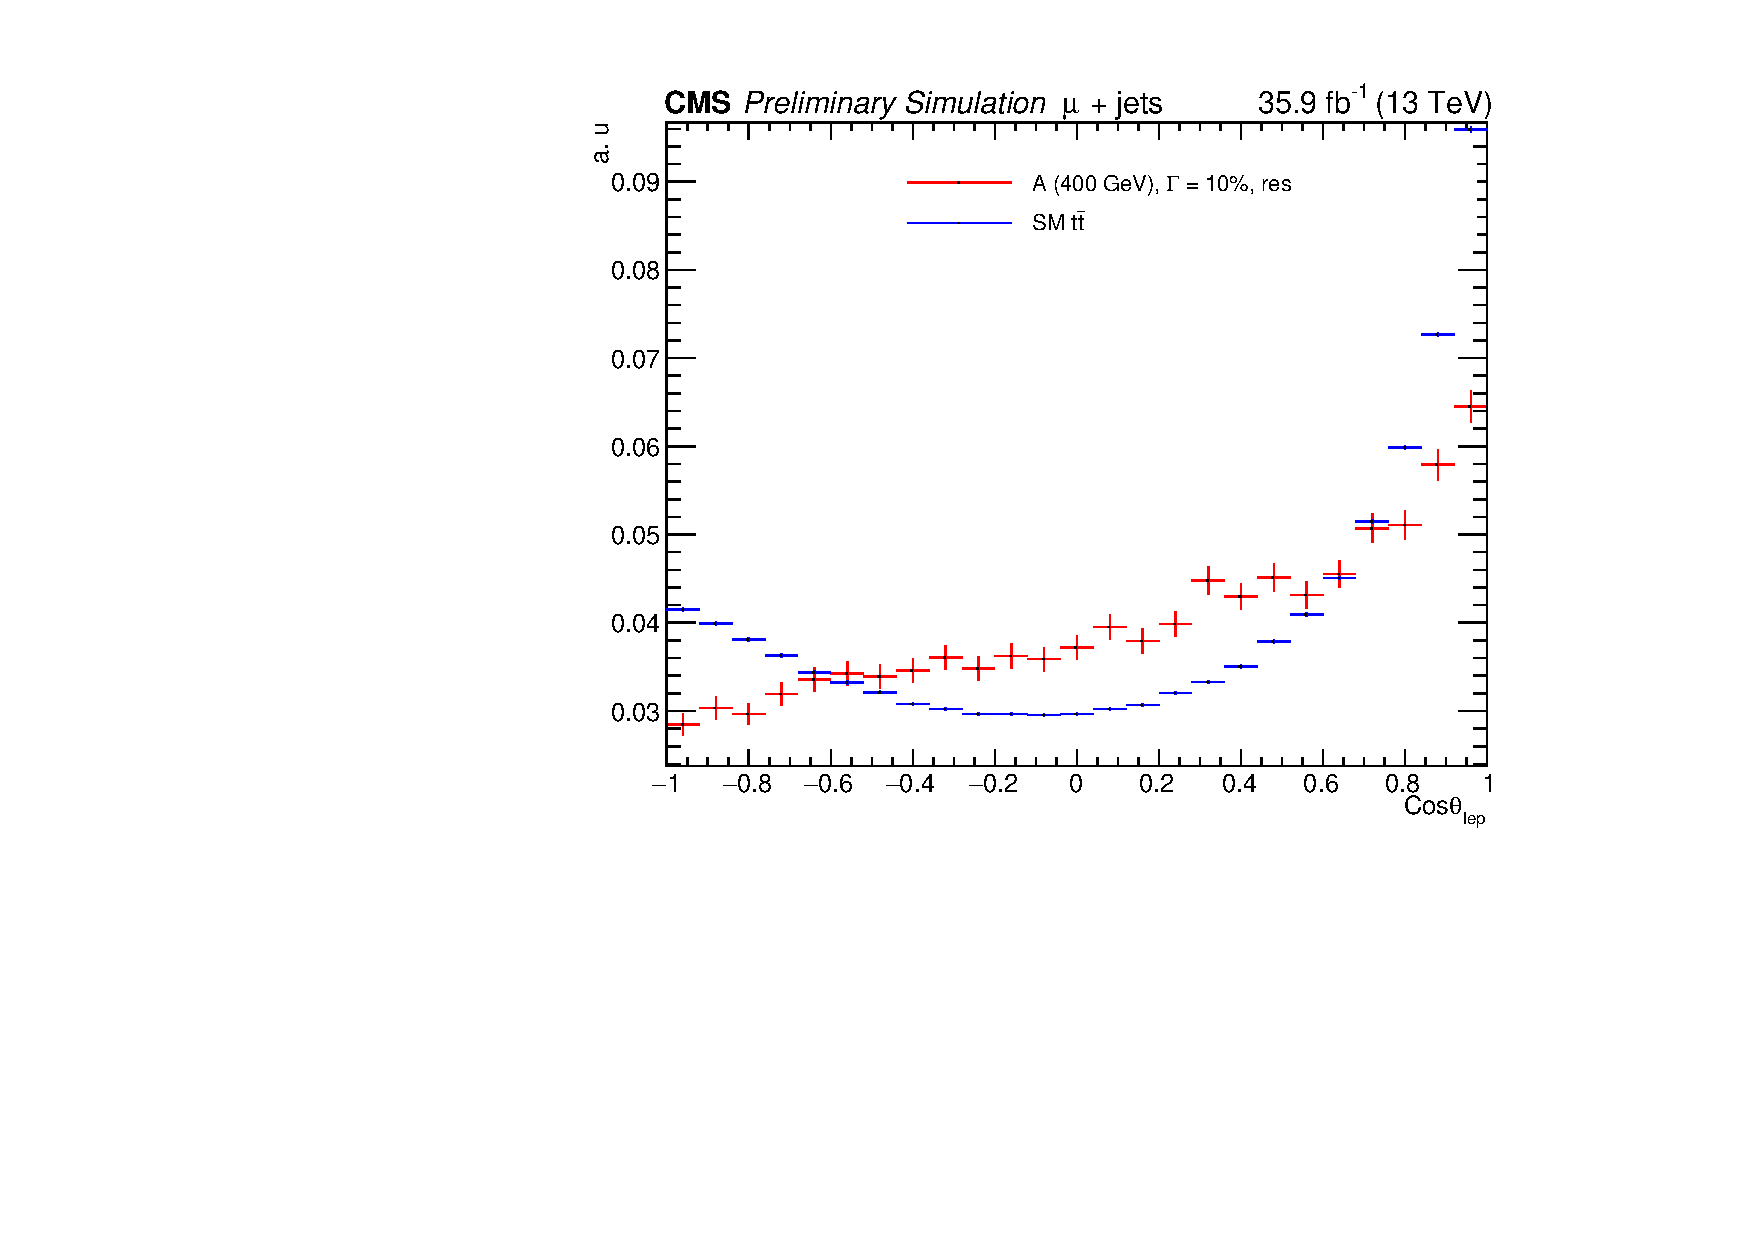
\includegraphics[scale=0.45]{fig/sm_beyond/cos_theta_pseudoscalar_M400_RelW10_res.pdf}
& \hspace{-2.cm} 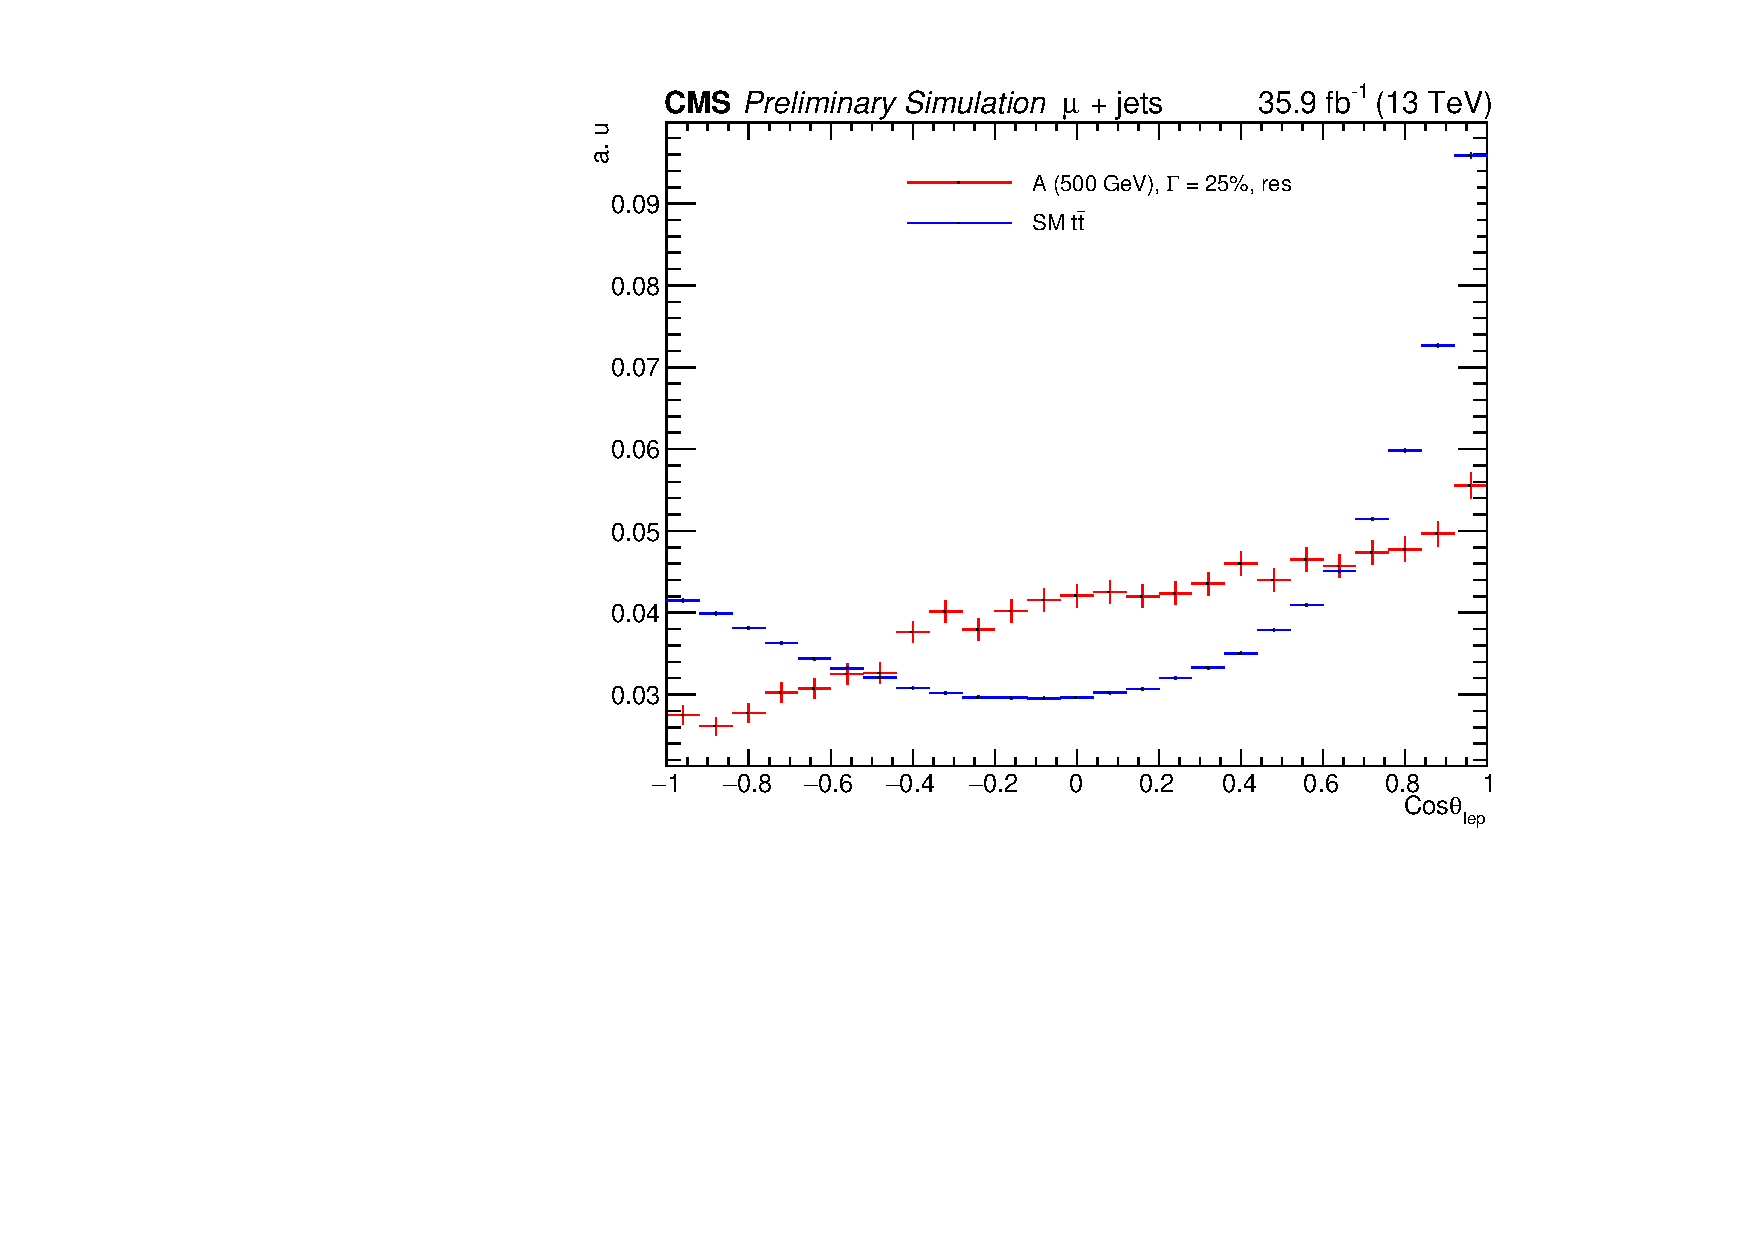
\includegraphics[scale=0.45]{fig/sm_beyond/cos_theta_pseudoscalar_M500_RelW25_res.pdf}\\
  \qquad ($\mathbf{a}$)\qquad&($\mathbf{b}$) \\
\end{tabular}
\caption{The $\cos\theta$ distribution, where $\theta$ is the leptonic top (the reconstruction of the $t\bar t$ system in the detector depends on the final state of the top quark. For the semileptonic decay mode, one top quark is reconstructed as leptonic and other one as hadronic, with more explanation provided in section~\ref{Sec:SearchVars}.) quark 3-momentum in the rest frame of the $t\bar t$. The red histogram shows the resonance pseudo-scalar (A) with mass = 400\,GeV and $\Gamma$ = 10\% in (a) and mass = 500\,GeV and $\Gamma$ = 25\% in (b). The blue line shows the SM $t\bar t$ distribution in both (a) and (b). Both histograms are scaled to one for shape comparison.}\label{fig:collins_soper}
\end{figure}
 %----------------------------------------------------------------------------------------------------------

\noindent \textbf{Sensitivity in the $gg\rightarrow A/H \rightarrow t\bar t$ channel:} In the previous section, production from the gluon-gluon fusion via top loop and decay to $t\bar t$ of the two $\mathcal{CP}$ states has been discussed in detail along with the SM $t\bar t$ interference. A large parameter space in [M$_{A}$, $\tan\beta$] is available to be probed at LHC high luminosity in this channel. A very simple analysis is performed in~\cite{Djouadi:2015jea} in order to find the sensitivity in the $t\bar t$ final state of a spin-one resonance based on ATLAS and CMS results~\cite{PhysRevD.88.012004,PhysRevLett.111.211804}. In a short introduction, spin-one resonance is produced by $q\bar q$ annihilation and doesn't interfere with the (coloured) QCD $q\bar q\rightarrow t\bar t$. Thus, a simple resonance peak appeared above the continuum SM $t\bar t$ background. For signal (masses = 400, 600 and 800\,GeV) and background $t\bar t$ processes, the events generated using $\textsc{MadGraph}$ generator. Signal production cross section and branching ratios have been calculated using $\textsc{HIGLU}$ and $\textsc{HDECAY}$ programs respectively. The background QCD $t\bar t$ cross section has been calculated using $\textsc{Top}$++ program with top quark mass m$_{t}$ = 173.2\,GeV, $\mu_{R}=\mu_{F}=m_{t}$ and at the order of NNLL including resummation scale. 

The number of signal and background events are simply taken with cuts on basic kinematic variables to suppress the $t\bar t$ QCD background and probed that region in the parameter space of [M$_{A}, \tan\beta$] in the hMSSM context where $N_{sig}/\sqrt{N_{bkg}}\geq s$. The results shown in Fig.~\ref{fig:Htt_sensitivity} for $\sqrt{\hat{s}} = 14$\,TeV use red, green, blue, and magenta lines for 2, 3, 4, and 5$\sigma$ sensitivity respectively, which is scaled to 300\,fb$^{-1}$ luminosity. With increasing luminosity, the situation could be vastly improved for sensitivity and a 2$\sigma$ `evidence' or 95\% CL exclusion limit can be achieved with $\tan\beta\approx 7$ with M$_{A}\approx 350$\,GeV in the MSSM context. A 5$\sigma$ discovery can be claimed at $\tan\beta \approx 6$ and M$_{A}\approx 350$\,GeV and at $\tan\beta \approx 1$ and M$_{A}\approx 800$\,GeV. 
\begin{figure}[htbp]
\centering
%\hspace{2.0cm}
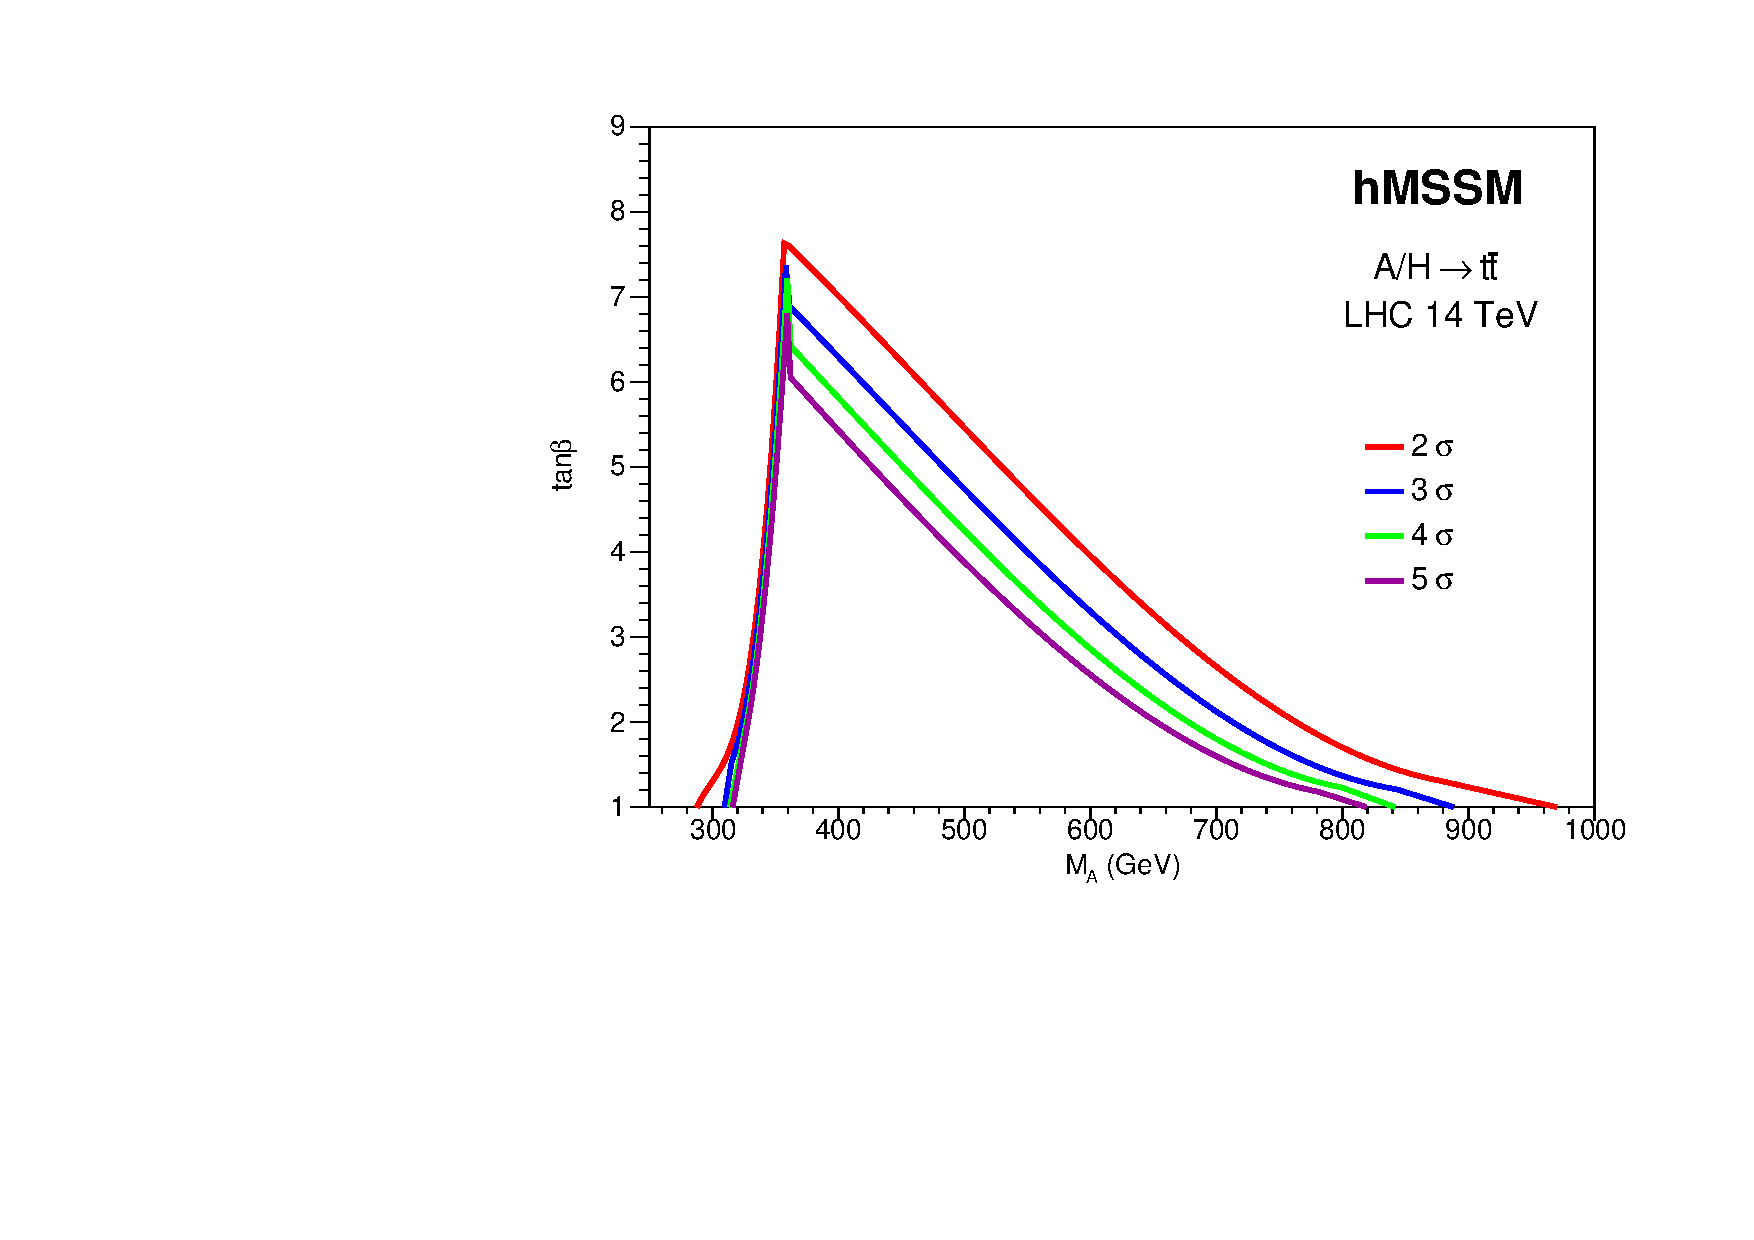
\includegraphics[trim={0cm 0.0cm 0 0.8cm},clip, scale=0.6]{fig/sm_beyond/plots_constraints_LHC14_300_AH_tt.pdf}
\caption{Sensitivity levels for $\Phi\rightarrow t\bar{t}$ channel at $\sqrt{s}=14$\,TeV with total integrated luminosity $\mathcal{L}$=300\,$\text{f}\text{b}^{-1}$ in hMSSM on [$\text{M}_{A}, \tan\beta$] plane. At M$_{\Phi} \approx 2\text{m}_{t}$, we have a large $\tan\beta$ space up to 7.5, which shows the sensitivity of the top quark to new physics~\cite{Djouadi:2015jea}. In the absence of new physics, the area under the contours will be excluded with corresponding sensitivity.}\label{fig:Htt_sensitivity}
\end{figure}
%-------------------------------------------------------------------------------

\noindent \textbf{Constraints on A/H/H$^{\pm}$ and projections at 0.3 and 3.0 ab$^{-1}$:}
CMS and ATLAS performed searches for heavy neutral and charged Higgs in different decay channels, fermionic decay channel $A/H\rightarrow \tau\tau$ and $H^{\pm}\rightarrow \tau\nu$ and bosonic decay channel $H\rightarrow WW, ZZ, hh$ and $A\rightarrow Zh$, that excluded a large parameter space in [M$_{A}$, $\tan\beta$]. For large $\tan\beta$ and high mass range, $A/H\rightarrow \tau \tau$ is the most sensitive channel that excludes a large parameter space. The bosonic channels are effective in lower $\tan\beta$ areas, while $H^{\pm}\rightarrow \tau\nu$ channel is sensitive to all $\tan\beta$ values at low masses. The virgin area in [M$_{A}$, $\tan\beta$] for M$_{A}\gtrsim 350$ and $\tan\beta \lesssim 4$ is not covered by the aforementioned channels. The $gg\rightarrow A/H\rightarrow t\bar t$ channel perfectly occupies this area because of the high $t\bar t$ mass threshold, $\approx 350$\,GeV, demanding a heavier Higgs and coupling of top quark to Higgs proportional to $1/\tan\beta$ (a lower $\tan\beta$ is the best option). It is shown in Fig.~\ref{fig:heavy_higgs8tev_exclusion} by a red-dashed contour in the parameter space of [M$_{A}$, $\tan\beta$] in the context of hMSSM along with the shadow area excluded by the combined searches of the CMS and ATLAS collaborations at $\sqrt{s}$ = 7+8\,TeV at 25\,fb$^{-1}$ luminosity up to 2$\sigma$ sensitivity. 
\begin{figure}[htp]
\centering
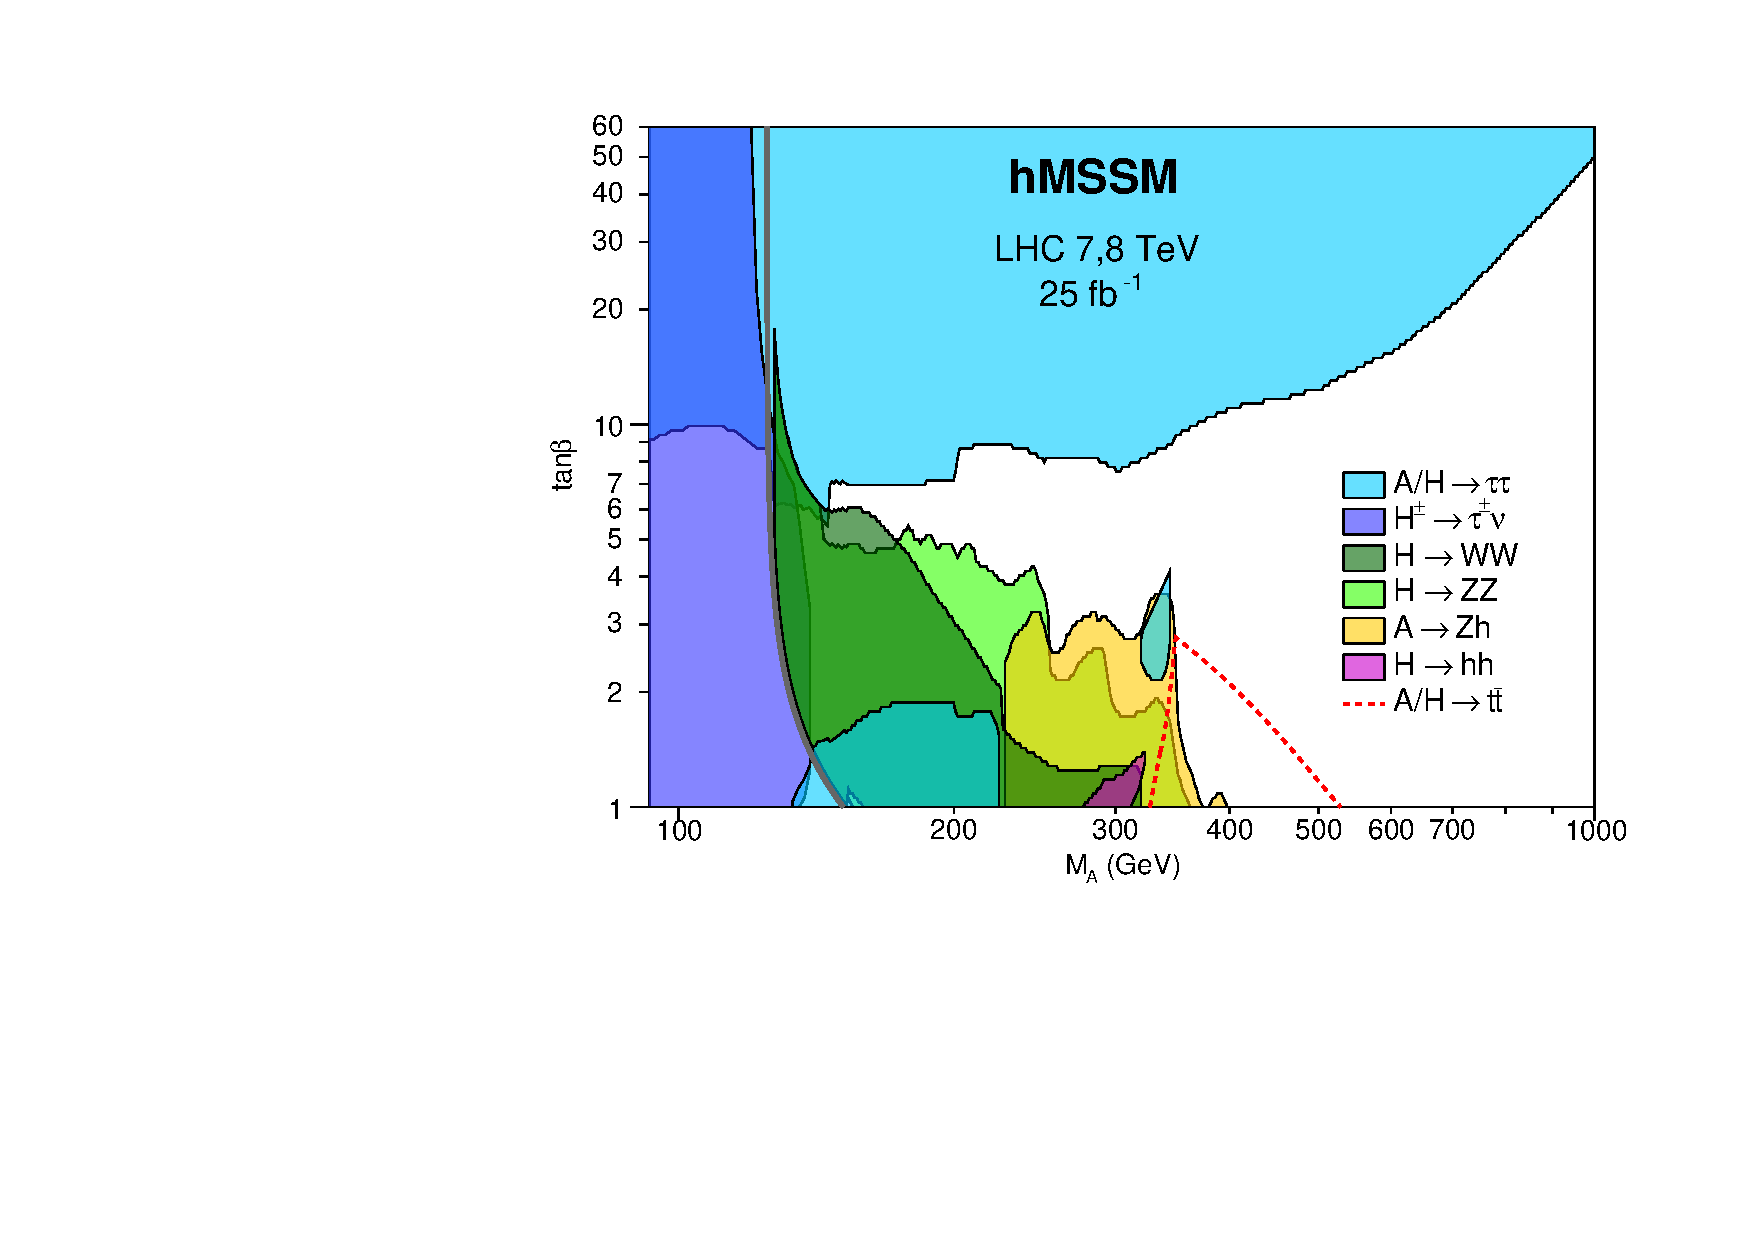
\includegraphics[trim={0cm 0.0cm 0 0},clip, scale=0.5]{fig/sm_beyond/httplots_constraints_LHC8_all.pdf}
\caption{
The combined constrains applied by the collaboration of CMS and ATLAS on the heavy Higgs, A, H, H$^{\pm}$, in the parameter space of [M$_{A}$, $\tan\beta$] in the context of hMSSM, target fermionic and bosonic channels. All the searches are performed up to $\sqrt{s}$ = 8\,TeV using 25\,fb$^{-1}$ data. The $gg\rightarrow A/H\rightarrow t\bar t$ channel is shown by a red-dashed contour that covers the high mass and low $\tan\beta$ range where other channels are not reachable\cite{Djouadi:2015jea}. 
}\label{fig:heavy_higgs8tev_exclusion}
\end{figure}

During the next phase of LHC when the integrated luminosity reaches 0.3 and 3.0\,ab$^{-1}$, the exclusion limit will be vastly improved in the absence of new signal, especially the 2$\sigma$ sensitivity will be drastically enhanced in the next LHC run. To extrapolate the 95\%CL exclusion limit for the MSSM Higgs, put together by CMS and ATLAS searches at $\sqrt{s}$ = 8\,TeV and $\mathcal{L}\approx$ 20\,fb$^{-1}$, to $\mathcal{L}\approx$ 0.3 ab$^{-1}$ at $\sqrt{s}$ = 14\,TeV, a naive approach has been adopted. The assumption made on the basis that ``the results of the experimental analyses are limits on the signal cross section at a given centre-of-mass energy, $\sqrt{s}$, and fixed integrated luminosity value $\mathcal{L}_{\sqrt{s}}$ for a given resonance mass bin, R$^{S}_{\sqrt{s}}$(M$_{A}$), for a channel that is subject to a given background rate R$^{B}_{\sqrt{s}}$(M$_{A}$) at this mass bin.'' Once we have knowledge about the R$^{S}_{8}$(M$_{A}$) at 8\,TeV, an extrapolation related to 14\,TeV can be written as:
\begin{equation}\label{equ:extrapolation_to14TeV_bkg}
R^{S}_{14}(M_{A}) = \sqrt{\mathcal{L}_{8}/\mathcal{L}_{14}} \sqrt{R^{B}_{14}(M_{A})/R^{B}_{8}(M_{A})} R^{S}_{8}(M_{A}).
\end{equation}

Further assumption is made for the unknown background rates based on the known signal cross section at certain points, ``the background rate increasing linearly to the signal cross section''. This assumption is suitable in the $gg\rightarrow A/H\rightarrow t\bar t$ channel, where the main background is also produced by the gluon-gluon fusion, $gg\rightarrow t\bar t$, which increases with increasing in energy at LHC. However, this approach is conservative for those channels whose main background is from $q\bar q$ annihilation like $H\rightarrow WW, ZZ$ or $A/H\rightarrow\tau\tau$ because with an increase in energy, the rate increases very slowly. With these assumptions, Eq.~\ref{equ:extrapolation_to14TeV_bkg} can be written as:
\begin{equation}\label{equ:extrapolation_to14TeV_sig}
R^{S}_{14}(M_{A}) \approx \sqrt{\mathcal{L}_{8}/\mathcal{L}_{14}} \sqrt{\sigma^{S}_{14}(M_{A})/\sigma^{S}_{8}(M_{A})} R^{S}_{8}(M_{A}).
\end{equation}

Using this approach, the combined CMS and ATLAS results at $\sqrt{s}$ = 8\,TeV and $\mathcal{L}\approx$ 20\,fb$^{-1}$ are extrapolated to 0.3 and 3.0\,ab$^{-1}$ in~\ref{fig:heavy_higgs14tev_exclusion}(a) and (b) respectively on [M$_{A}$, $\tan\beta$] plane in the context of hMSSM. In Fig.~\ref{fig:heavy_higgs14tev_exclusion} an extra channel, $H^{\pm}\rightarrow tb$, is added in comparison to Fig.~\ref{fig:heavy_higgs8tev_exclusion}, shown by the dark-blue area. At high luminosity, the results are optimistic and at 95\% CL, the sensitivity of most channels is highly improved. The $A/H\rightarrow \tau\tau$ channel now covers the whole parameter space in [M$_{A}$, $\tan\beta$] for M$_{A}\lesssim 350$\,GeV. The sensitivity of $gg\rightarrow A/H \rightarrow t\bar t$ channel increases and at 0.3\,ab$^{-1}$, it can probe $\tan\beta \lesssim$ 8 and M$_{A}$ 350-1000\,GeV in [M$_{A}$, $\tan\beta$] space, while for 3.0\,ab$^{-1}$, its sensitivity is further enhanced to $\tan\beta \lesssim$ 12 and M$_{A}$ 350-1500\,GeV. Examining the extrapolated results, especially for 3.0\,ab$^{-1}$, the $gg\rightarrow A/H\rightarrow t\bar t$, the channel receives more attention and will play a pivotal role in the heavy Higgs searches. 
\begin{figure}[htp]
\centering
\begin{tabular}{cc}
\hspace{-0.3cm}
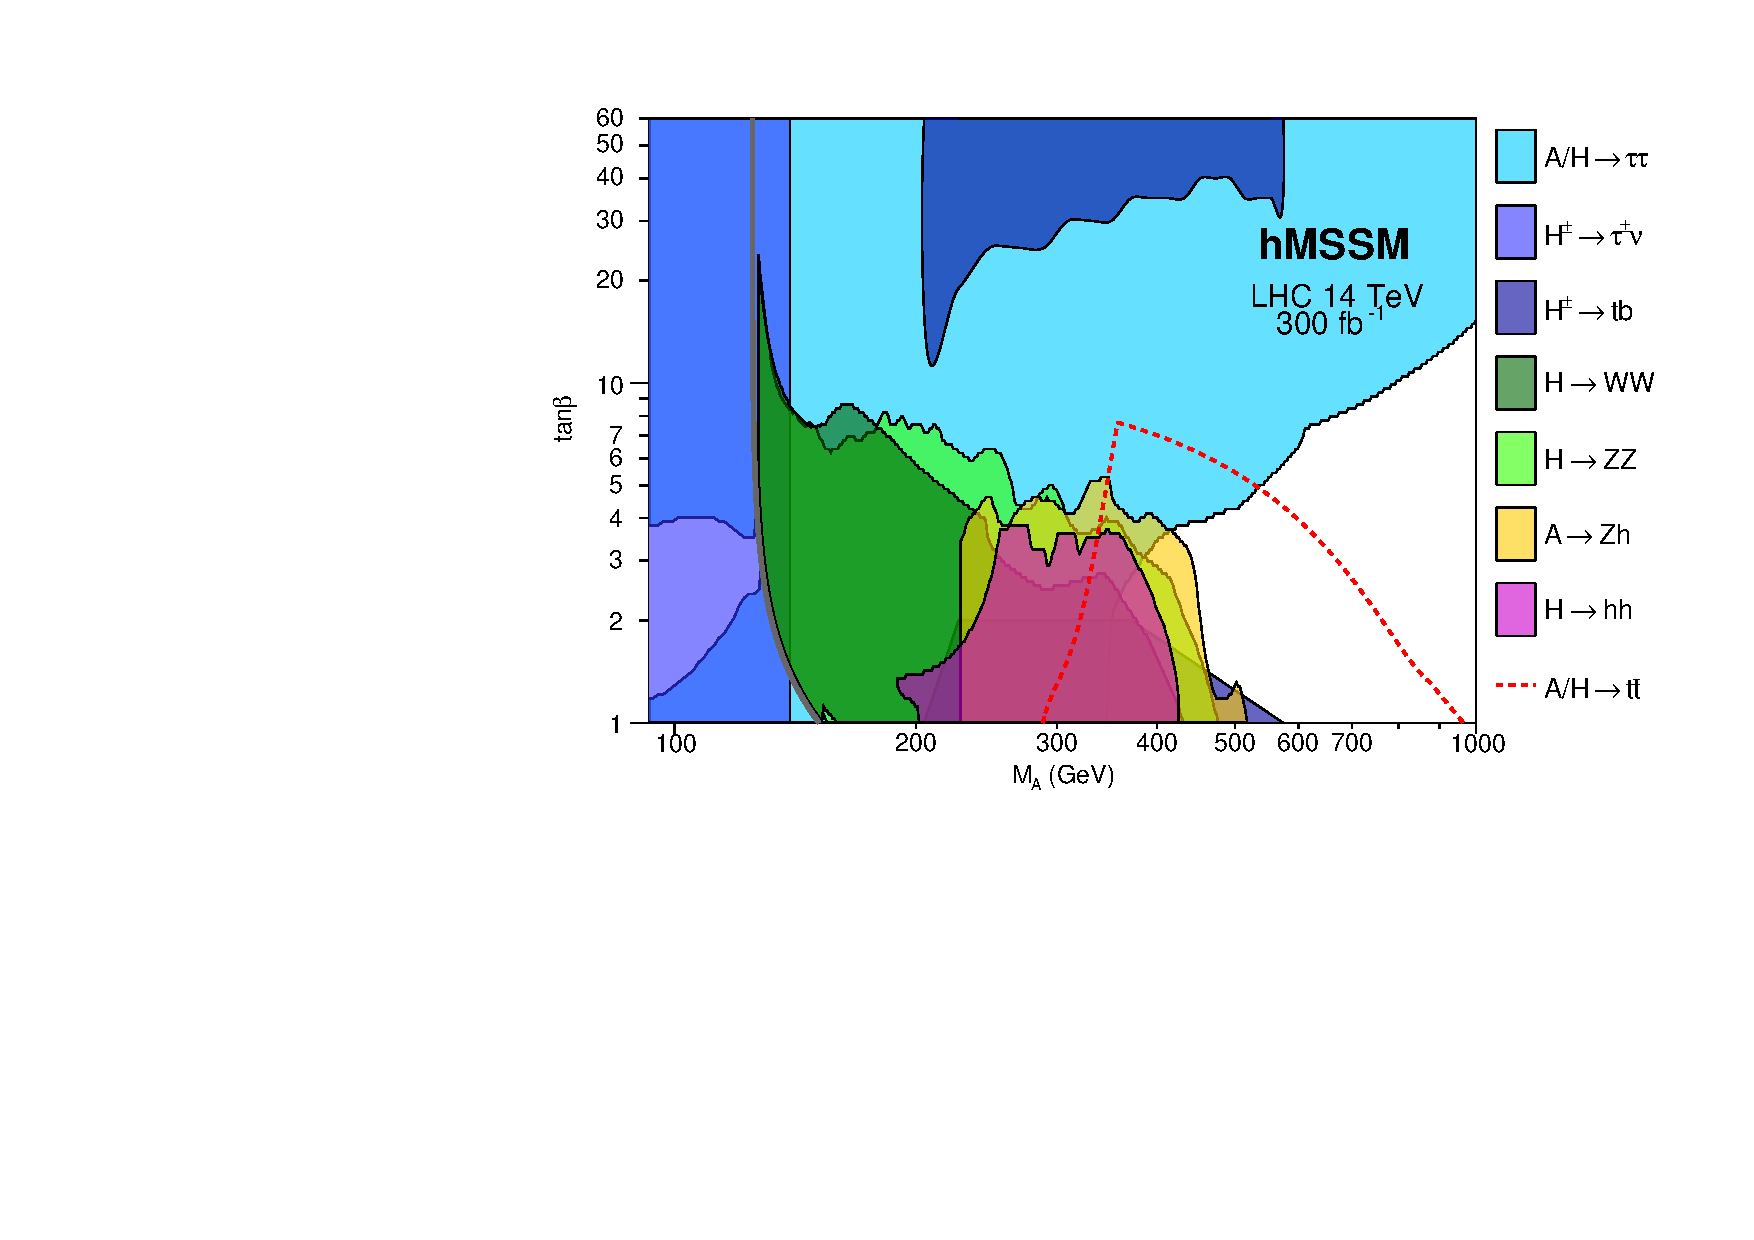
\includegraphics[trim={0cm 0.0cm 0 0},clip, scale=0.43]{fig/sm_beyond/httplots_constraints_LHC14_300fb_all.pdf}
& \hspace{-2.2cm} 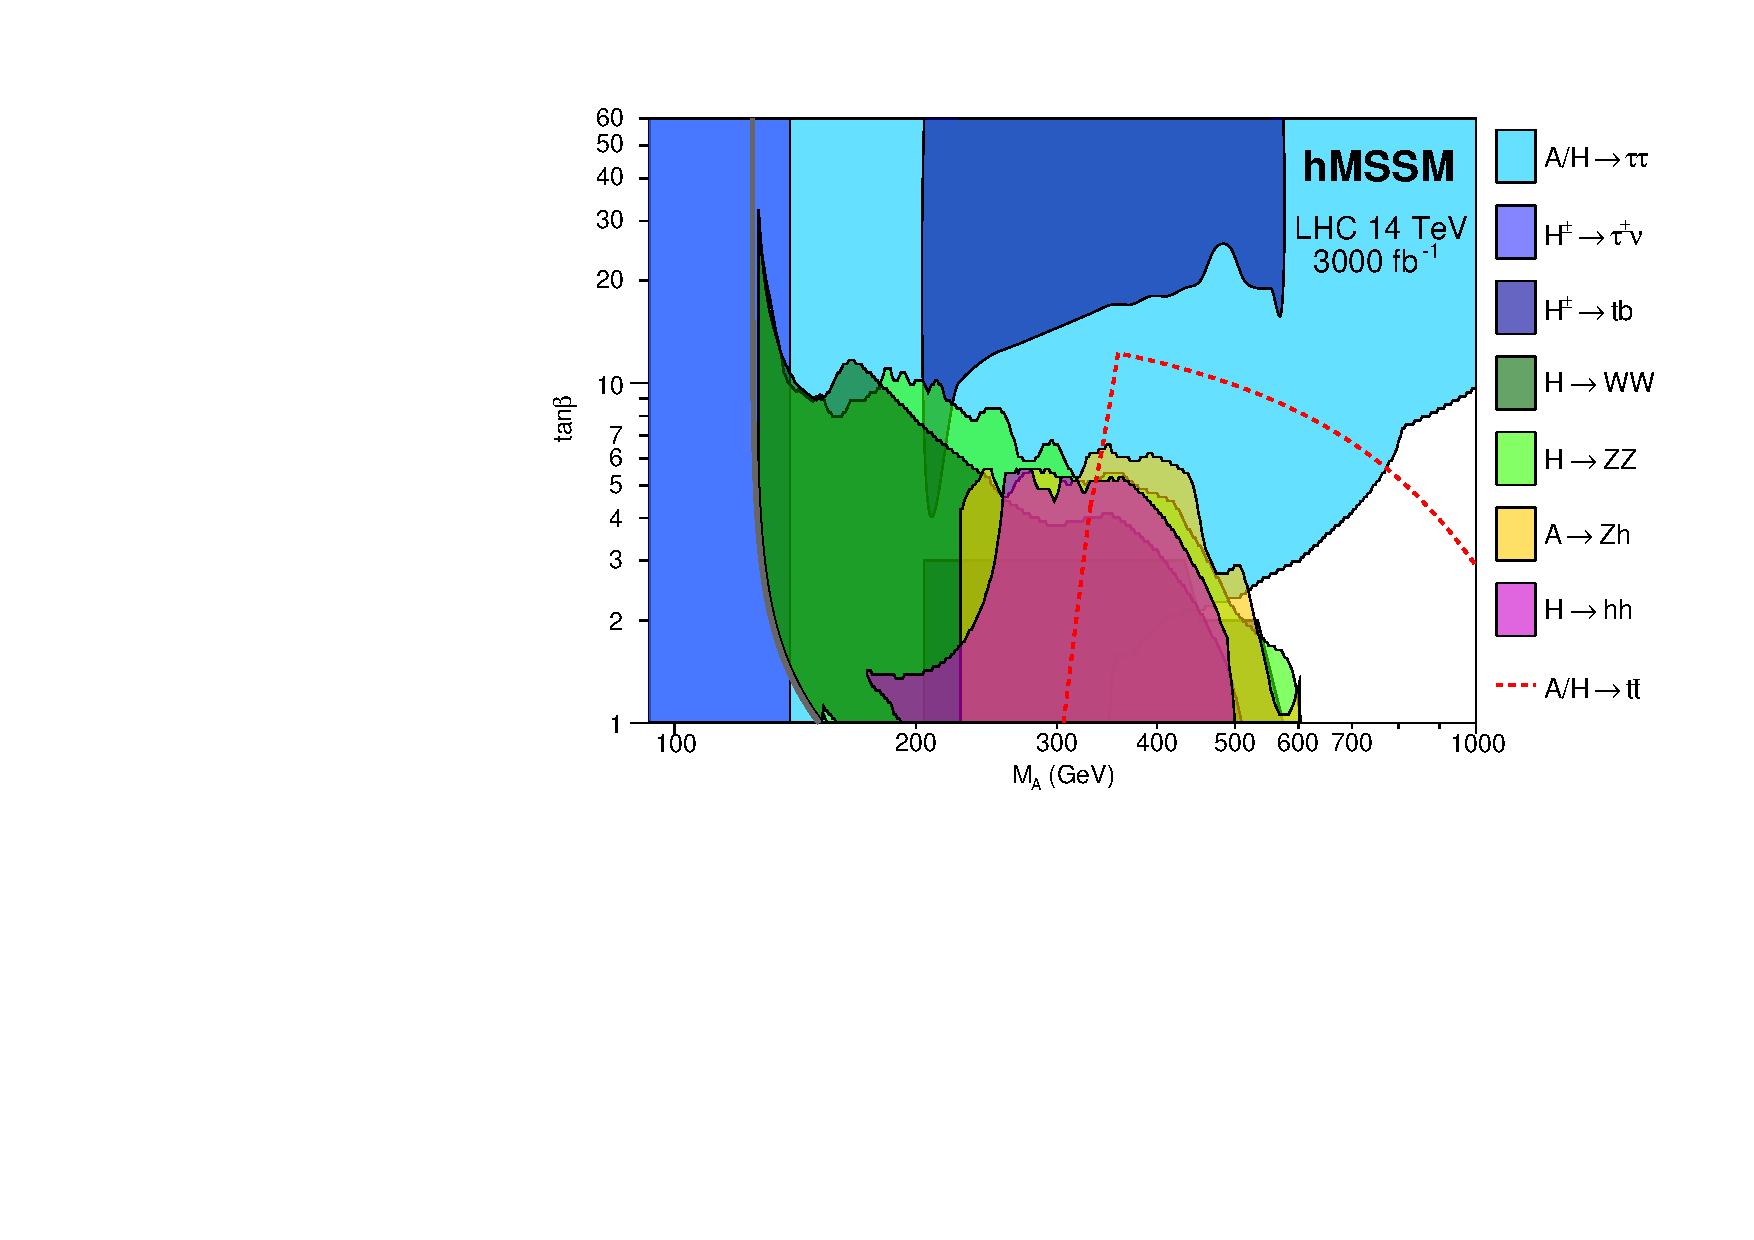
\includegraphics[trim={0cm 0.0cm 0 0},clip, scale=0.43]{fig/sm_beyond/httplots_constraints_LHC14_3000fb_all.pdf}\\
  \qquad ($\mathbf{a}$)\qquad\qquad&($\mathbf{b}$)\qquad\qquad\qquad\qquad \\
\end{tabular}
\caption{Extrapolated from 8\,TeV and $\approx$ 20\,fb$^{-1}$ data, the combined CMS and ATLAS results for neutral and charged Higgs searches with expectation of 2$\sigma$ at $\sqrt{s}=14$\,TeV using hMSSM with total integrated luminosity $\mathcal{L}=300 \text{f}\text{b}^{-1}$ (a) and  HL-LHC $\mathcal{L}=3000 \text{f}\text{b}^{-1}$ (b) in the [$\tan\beta, \text{M}_{A}$] plane. The red-dashed contour shows the $\Phi\rightarrow t\bar{t}$ channel projection, where its sensitivity increases as compared to 8\,TeV~\cite{Djouadi:2015jea}. }\label{fig:heavy_higgs14tev_exclusion}
\end{figure} 
%\clearpage{\pagestyle{empty}\cleardoublepage}
